\documentclass[sn-mathphys,Numbered]{sn-jnl}
\usepackage{graphicx}
\usepackage{multirow}
\usepackage{amsmath,amssymb,amsfonts}
\usepackage{amsthm}
\usepackage{subcaption}
\usepackage{mathrsfs}
\usepackage[title]{appendix}
\usepackage{xcolor}
\usepackage{textcomp}
\usepackage{manyfoot}
%\usepackage{subfig}
\usepackage{booktabs}
\usepackage{algorithm}
\usepackage{algorithmicx}
\usepackage{algpseudocode}
\usepackage{listings}
\usepackage[section]{placeins}
\theoremstyle{thmstyleone}
\newtheorem{theorem}{Theorem}
\newtheorem{proposition}[theorem]{Proposition}
\theoremstyle{thmstyletwo}
\newtheorem{example}{Example}
\newtheorem{remark}{Remark}
\theoremstyle{thmstylethree}
\newtheorem{definition}{Definition}
\raggedbottom

\begin{document}
\title[Article Title]{Multi-Bidirectional shifting based data transformation (MBiS-DT) for temperature prediction using ensamble deep learning}
\author*[1,2]{\fnm{Rana} \sur{Kumar}}\email{singhranakumar22@gmail.com}
\author[1,2]{\fnm{Vipin} \sur{Kumar}}\email{rt.vipink@gmail.com}
%\equalcont{These authors contributed equally to this work.}

%\author[1,2]{\fnm{Third} \sur{Author}}\email{iiiauthor@gmail.com}
%\equalcont{These authors contributed equally to this work.}

\affil*[1]{\orgdiv{Computer Science \& Information Technology}, \orgname{Mahatma Gandhi Central University}, \orgaddress{\state{Bihar}, \country{India}}}

%\affil[2]{\orgdiv{Computer Science \& Information Technology}, \orgname{Mahatma Gandhi Central University}, \orgaddress{\state{Bihar}, \country{India}}}

%\affil[3]{\orgdiv{Department}, \orgname{Organization}, \orgaddress{\street{Street}, \city{City}, \postcode{610101}, \state{State}, \country{Country}}}

%%==================================%%
%% sample for unstructured abstract %%
%%==================================%%

\abstract{Accurate temperature prediction holds key significance in distinct sectors such as power requirement in city and industry, with deep implications for global climate understanding. This paper presents an innovative approach to enhance the temperature prediction through the vareious deep learning techniques: Long Short-Term Memory (LSTM), Recurrent Neural Networks (RNN), Gated Recurrent Unit (GRU) and Bi-directional Long Short Term Memory (BiLSTM). These deep learning techniques have capability in capturing complex temporal dependencies complements \cite{xu2019improving} , modifying overfitting concerns. The proposed Paradigm Shift hybrid models capitalizes on the strengths of traditional deep learning methods, seeking to boost their predictive capability and reduce variance-related errors.Our study dig in into the complex stuff of time-series satellite data, particularly focusing on Delhi city temperature deviation. Informed by the relatively indefinite variation of City Temperature, we influence Paradigm Shift to get new shifted dataset. Traditional BI LSTM (BI-LSTM) is introduced, enhancing the predictive power by placing emphasis on local data interactions \cite{tabrizi2021hourly}. The BI-LSTM methodology performs the best because it adopts a quadratic cost function and strategically weighting training sample data proximate to test different point.}



\keywords{Time-Series, Deep Learning, LSTM, BI-LSTM, GRU, RNN}

%%\pacs[JEL Classification]{D8, H51}

%%\pacs[MSC Classification]{35A01, 65L10, 65L12, 65L20, 65L70}

\maketitle

\section{Introduction}\label{sec1}

Temperature prediction is a fundamental aspect of weather forecasting and climate research, essential for various applications across diverse domains, ranging from agriculture and energy management to public health planning and urban infrastructure development. Accurate temperature forecasts enable us to make informed decisions, proactively respond to extreme weather events, and adapt to changing climate patterns. While traditional statistical methods have been the cornerstone of weather prediction, recent advancements in deep learning have opened up new broadway for enhancing the accuracy and reliability of temperature forecasting. Likewise, impacts on the food security, human health, economy, and energy consumption are anticipated \cite{cifuentes2020air}.

In this paper, we delve into the application of deep learning techniques for temperature prediction using time series data from the bustling metropolis of Delhi, India. Delhi, being the capital city and one of the most populous urban centers in India, experiences diverse weather patterns influenced by both natural climate variability and anthropogenic activities. Understanding and predicting temperature trends in this region is crucial for effective urban planning, resource management, and mitigating the impacts of heatwaves and cold spells on public health and infrastructure.This paper embarks on a journey into the realm of deep learning, a revolutionary field of artificial intelligence that has exhibited remarkable prowess in modeling complex temporal data. By applying deep learning techniques to the rich time series data of temperature in Delhi, this research endeavor seeks to unlock valuable insights that can drive informed decision-making.The core motivation of this paper is rooted in the realization that climate science is far from linear; it embodies intricate non-linearities and dynamic interplays. This complexity makes neural networks, particularly deep learning models, an ideal choice to capture the nuanced relationships within temperature time series data. Deep learning, with its capacity to unveil hidden patterns, is uniquely poised to discern the subtleties of climate systems and predict temperature fluctuations with unprecedented accuracy.Crucially, this paper not only explores the application of deep learning but also delves into the integration of advanced training algorithms. The fusion of backpropagation with genetic algorithms brings forth a robust and adaptable framework for model training, ensuring that our temperature predictions are not only accurate but also resilient to the complexities of climate systems. air temperature prediction is a main climate factor essential for many types of applications in multiple area such as tourism,  industry, agriculture,  environment,  energy etc. \cite{abdel2004hourly}.

The use of deep learning in temperature prediction is usefull due to its inherent capability to capture intricate temporal dependencies and nonlinear relationships within data. In the past few years, advanced machine learning models like Artificial Neural Networks (ANNs), Long Short-Term Memory (LSTM) networks\cite{wang2017predrnn} \cite{chen2021study}, and Convolutional Neural Networks (CNNs)\cite{chen2021correction} have shown great success across various areas. An example of this is the LSTM model, which was introduced by Sepp Hochreiter and Jiirgen Schrnidhuber\cite{graves2012long} in 1997. LSTM is particularly good at handling sequences of data, like those found in time series analysis.Among the array of deep learning architectures, we explore the Long Short-Term Memory (LSTM) network, celebrated for its capability in modeling sequential data. Our investigation extends beyond the utilization of LSTM to introduce the BI-LSTM, an innovative approach that integrates local information for enhanced time series prediction. BI-LSTM offers a unique perspective by assigning higher importance to samples proximate to the test points, effectively capturing localized patterns critical for accurate forecasting.The methodology applied in this paper include thorough data collection and preprocessing, essential for ensuring the integrity of our analysis. We get historical temperature data from reliable weather stations in Delhi from NASA's website, covering a specific time span conducive to meaningful climate insights. correct data cleaning tunes the missing values, outliers, and duplicates, while feature extraction results the temperature-related attribute Temperature at 2 meter (T2M).Exploratory Data Analysis (EDA) forms an integral part of our investigation, revealing underlying patterns, trends, and seasonality within the temperature time series data. Our visualizations and statistical analyses provide valuable insights into the data's temporal behavior.The core of our research resides in the deep learning model development, specifically the LSTM,BI-LSTM,GRU and RNN architectures. We detail our model selection criteria, including hyperparameter tuning, to enhance prediction accuracy. The dataset undergoes partitioning into training, testing sets, facilitating the model training and testing process.To ensure the reliability of our predictions, we conduct a thorough evaluation using performance metrics such as Root Mean Square Error (RMSE), Mean Squared Error(MSE), Mean Absolute Error (MAE), and Mean Absolute Percentage Error (MAPE).


Through this paper, we aim to investigate the effectiveness of employing deep learning models in predicting temperature patterns in Delhi. By utilizing historical temperature data collected from various meteorological stations, we seek to train and evaluate the performance of DL models and compare their results with traditional forecasting methods. The insights gained from this study will shed light on the strengths and limitations of deep learning-based temperature predictions and provide valuable guidance for future research and practical implementations.
\subsection{The novelty of proposed research work:}

\begin{itemize}
\item A comprehensive performance study of different measures of the Deep Learning Models has been done where the better performer has been identified successfully based on RMSE,MAE. Now our goal is to develop a hybrid model which have better value of RMSE,MAE to predict better result.
\item opening new path for Multi Bi-directional shifting on data to apply ensemble deep learning models .
\end{itemize}
The residual of this paper is ordered as follows: Section 2 - provides a list of recent works Previous work, as well as a review of the literature. Section 3 gives the DL models and performance measures. Section 4 includes steps of experiment and mplamentation setup and parameters settings . Section 5 presents the experimental results and their thorough analysis. The sixth section concluded with a review of existing and future research endeavours.

\section{Previous Work}
Many research has been undertaken to predict temperature using past data as a critical temperature attribute. Researchers require effective study and data to procced their investigation on a dataset of temperature of city \cite{cifuentes2020air}. The temperature is used as a parameter to identify the climate change,  green house effect, crop yield etc.
\cite{2019AGUFMGC33A..05P}This study explored the application of deep learning models for extreme weather prediction, including temperature extremes. Extreme weather events, such as heatwaves and cold spells, have significant impacts on society and require accurate forecasting for effective preparation and response. The authors experimented with LSTM networks and Convolutional Neural Networks (CNNs) to predict extreme weather events. LSTMs were employed to capture temporal dependencies, while CNNs were used to extract spatial patterns from meteorological data. The research demonstrated that deep learning models outperformed traditional methods in predicting temperature extremes, showcasing the potential of these models in enhancing weather forecasting systems to address severe weather events.

\cite{salinas2020deepar} This work introduced DeepAR, a probabilistic forecasting model based on autoregressive recurrent networks. The model is capable of providing not only point predictions but also probability distributions for uncertainty estimation. For temperature prediction, uncertainty estimation is crucial, as it provides valuable information for decision-making in weather-sensitive applications. DeepAR offers a principled approach for capturing the uncertainty in predictions, making it suitable for applications where risk assessment is important .

\cite{singh2011time} This paper addresses the temporal and time-series nature of temperature prediction and its critical role in today's agricultural and industrial sectors. Leveraging neural networks due to the non-linearities in climatic physics, the paper introduces a significant approach: the integration of backpropagation with genetic algorithms for training these networks. The central contribution is a time series-based temperature prediction model employing this integrated technique.The paper's focus includes demonstrating the interdependence of temperature and specific data sequences, emphasizing the implications of accurate forecasting for key sectors. It further explores the suitability of neural networks in capturing intricate meteorological processes. The proposed technique sheds light on the effects of undertraining and overtraining, highlighting the model's sensitivity to proper training.

  \cite{XIAO2019111358}This paper proposes a novel approach for predicting short and mid-term daily sea surface temperature anomalies (SSTA) using a combination of the LSTM deep recurrent neural network model and the AdaBoost ensemble learning model (LSTM-AdaBoost). The goal is to improve predictive accuracy by leveraging LSTM's ability to capture long-term dependencies and AdaBoost's robust prediction capability, while mitigating overfitting. The method involves modeling SSTA seasonality, training LSTM and AdaBoost independently, and combining their predictions using an averaging strategy. The study demonstrates the effectiveness of the LSTM-AdaBoost model in outperforming individual LSTM, AdaBoost, and other optimized models, offering promising potential for enhancing short and mid-term daily SST predictions in scenarios like extreme weather events.

  \cite{XIAO2019111358} The paper highlights the effectiveness of Long Short-Term Memory (LSTM) in capturing long-term dependencies, particularly in weather forecasting applications. Additionally, the study introduces Transductive LSTM (T-LSTM) as a novel approach that leverages local information in time-series prediction. T-LSTM operates in a transductive learning framework, attributing higher influence to nearby samples during model fitting. A quadratic cost function is used for regression, with the objective function localized by assigning larger weights to training samples near the test point. Two weighting schemes, based on cosine similarity, are explored \cite{XIAO2019111358}.
The research evaluates the proposed method's performance across varying weather conditions, conducting experiments over two different time periods within a year. The findings demonstrate that T-LSTM exhibits superior predictive performance compared to traditional LSTM, establishing its effectiveness in enhancing prediction accuracy for weather forecasting tasks.

\begin{table}[!h]
\centering
\caption{Literature Review Of Other Papers}\label{tab1}%
\begin{tabular}{ p{0.05\linewidth} p{0.1\linewidth} p{0.2\linewidth} p{0.12\linewidth}  p{0.45\linewidth} }
\toprule
Paper & MODELS  & Data Set Used & Measures & Research Gap \\
\midrule
\cite{li2019deep}    & LSTM   & china international airport temperature data from 2009-2018  & RMAE:1.2369, MSE:1.5365 & this paper could be the need for more accurate and stable temperature prediction models, specifically using stacked LSTM networks and their combination with other models.  \\
\cite{li2019deep}   & Random Forest   & china international airport temperature data from 2009-2018  &RMSE:1.3612, MSE:1.8645 & this paper could be the need for more accurate and stable temperature prediction models, specifically using stacked LSTM networks and their combination with other models.    \\
\cite{xiao2019spatiotemporal}    & LSTM   & East China Sea surface temperature data from 1982-2018   &RMSE:0.850  & this paper used satellite temperature data for prediction which is in graphical form so there is some complexity in graphical data over numeric data for deep  learning models. \\
\cite{thi2020deep}  & RNN       & Winter data of south korea from 1976-2015.     &RMSE:2.985, MSE:2.5777  & Time series forecasting of meteorological variables, such as daily temperature, has gained attention in recent years due to the limitations of traditional forecasting models. so need to some transformation in data or in traditional models.  \\
\cite{thi2020deep}  & LSTM    & Winter data of south korea from 1976-2015.      &RMSE:2.991, MSE:2.5525 & Time series forecasting of meteorological variables, such as daily temperature, has gained attention in recent years due to the limitations of traditional forecasting models. so need to some transformation in data or in traditional models. \\
\cite{hao2023temperature}  &  Bi-Conv-LSTM   &  ERA5 project of ECMWF, from January 1, 2018, to December 31, 2018 (365d in total)      &RMSE:2.75, MSE:7.56 & The paper focuses on the development of a hybrid conv-lstm model for temperature correction in meteorological forecasts.this paper could also ensemble with other models too or can adopt data transformation techniques.\\
\cite{zwart2023evaluating}  &  RG-CNN   &  enerated forecasts
using the National Oceanic and Atmospheric Administration’s
Global Ensemble Forecast System model version 12.0 0.25 degree reforecast archive \href{https://noaa-gefs-retrospective.
s3.amazonaws.com/index.html}{GEFS}      &RMSE:1.52, MSE:2.31 & The research gap in this paper is the need for further development of methods to optimally ingest observations from other sites to improve DL model forecasts at unmonitored locations\\

\cite{gong2022temperature}  &  ConvLSTM   &   ERA5      &RMSE:1.51, MSE:2.3 & The paper focuses on using a stacked long short-term memory network (Stacked LSTM) for temperature prediction and compares it with deep neural network (DNN) and random forest (RF) algorithms. here could be ensemble of DL models.\\
\botrule
\end{tabular}
%\footnotetext{Source: This is an example of table footnote. This is an example of table footnote.}
%\footnotetext[1]{Example for a first table footnote. This is an example of table footnote.}
%\footnotetext[2]{Example for a second table footnote. This is an example of table footnote.}
\end{table}
\section{Deep Learning Models}

\subsection {Recurrent Neural Networks (RNN):}
Recurrent neural networks (RNN) is an ANN, in which the outputs of past steps are fed as inputs to the current phase. The special feature of RNN is the feedback connection that transfers information about the previous step input, which is adapted by the succeeding input. RNN also have a memory or hidden state vector that retrieves some sequential data and computes new states by applying recursively its activation functions to previous states and new inputs. In this way, the RNN can process information in sequence and represent it's temporal behave for  time series, preserving information from previous data \cite{thi2020deep}.
The equation for a simple Recurrent Neural Network (RNN) is as follows:
\begin{equation}
h_t=\sigma(W_{hh} \cdot h_{t-1} + W_{hx} \cdot x_t + b_h)
\end{equation}

Where, \(x_t\) represents the input at time step \(t\).
 \(W_{hh}\) and \(W_{hx}\) is the weight matrix for the recurrent and input connection respectively.
 \(h_t\) is the hidden state at time step \(t\).
 \(b_h\) is the bias vector.
 \(\sigma\) is the activation function, commonly the sigmoid function.

\subsection{Gated Recurrent Unit (GRU):}

The Gated Recurrent Unit (GRU) is a neural network design addressing vanishing gradient challenges in sequence data modeling. It employs update and reset gates to control information flow within the network. The update gate balances new input against the previous state, while the reset gate decides what past information to ignore. The model's computations involve gate calculations, generating a candidate hidden state, and merging it with the previous state using the update gate. This architecture efficiently captures temporal patterns and long-range dependencies, making it popular for tasks involving sequential data like natural language processing and time series analysis. Its simplified structure and effectiveness offer an alternative to more complex architectures like LSTM. Equations of GRU are as follows:
\begin{equation}
z_t = \sigma(W_z \cdot [h_{t-1}, x_t]  +  b_z) 
\end{equation}
\begin{equation}
r_t = \sigma(W_r \cdot [h_{t-1}, x_t] +   b_r) 
\end{equation}
\begin{equation}
\tilde{h}_t = \tanh(W_h \cdot [r_t \odot h_{t-1}, x_t]  +  b_h) \\
\end{equation}
\begin{equation}
h_t = (1 - z_t) \odot h_{t-1} + z_t \odot \tilde{h}_t
\end{equation}



Where, \(x_t\) represents the input at time step \(t\).
 \(z_t\) is the update gate's output at time step \(t\).
 \(h_t\) is the hidden state at time step \(t\).
 \(\tilde{h}_t\) is the candidate hidden state at time step \(t\).
 \(r_t\) is the reset gate's output at time step \(t\).
 \(W_z\), \(W_r\), and \(W_h\) are weight matrices for the update gate, reset gate, and candidate hidden state calculations, respectively.
 \(b_z\), \(b_r\), and \(b_h\) are bias vectors for the corresponding gates and candidate hidden state.
 \(\sigma\) is the activation function(sigmoid).
 \(\odot\) represents multiplication element-wise .


\subsection{Long Short Term Memory (LSTM):}
Long Short-Term Memory (LSTM) is a specialized recurrent neural network architecture addressing vanishing gradient problems. It introduces memory cells and three gates: input, output, and forget. The input gate regulates new information intake, the output gate controls the information output, and the forget gate manages the memory's relevance. The cell state maintains long-term dependencies, enhancing the model's ability to capture sequences \cite{guillen2020deep}. LSTMs address challenges faced by traditional RNNs by allowing selective information update through gates and consistent gradient flow. This architecture is widely used for sequential data tasks, like language translation and speech recognition, due to its capacity for modeling context and handling extended sequences effectively \cite{qiu2021river}. The equations of LSTM are as follows:
\begin{equation}
f_t = \sigma(W_f \cdot [h_{t-1}, x_t] + b_f)
\end{equation}
\begin{equation}
i_t = \sigma(W_i \cdot [h_{t-1}, x_t] + b_i)
\end{equation}
\begin{equation}
\tilde{C}_t = \tanh(W_C \cdot [h_{t-1}, x_t] + b_C)
\end{equation}
\begin{equation}
C_t = f_t \odot C_{t-1} + i_t \odot \tilde{C}_t
\end{equation}
\begin{equation}
o_t = \sigma(W_o \cdot [h_{t-1}, x_t] + b_o)
\end{equation}
\begin{equation}
h_t = o_t \odot \tanh(C_t)
\end{equation}


Where, \(x_t\) represents the input at time step \(t\).
 \(i_t\) and \(f_t\) is the input gate's and forget gate's output at time step \(t\) respectively.
 \(h_t\) and \(C_t\) is the hidden and cell state at time step \(t\) respectively.
 \(C_t\) is the cell state at time step \(t\).
 \(\tilde{C}_t\) is the candidate cell state at time step \(t\).
 \(o_t\) is the output gate's output at time step \(t\).
 \(W_f\), \(W_i\), \(W_C\), and \(W_o\) are weight matrices for the gates and candidate cell state calculations.
 \(b_f\), \(b_i\), \(b_C\), and \(b_o\) are bias vectors for the corresponding gates and candidate cell state.
 \(\sigma\) is the sigmoid activation function.
 \(\odot\) represents element-wise multiplication.


\subsection{Bidirectional Long Short-Term Memory (BiLSTM):}
Bidirectional Long Short-Term Memory (BiLSTM) is an advanced neural network structure that overcomes vanishing gradient issues by processing data in both forward and backward directions. It consists of two LSTMs: one captures past information, and the other captures future context. Input sequences are processed in parallel, enabling the model to capture comprehensive temporal patterns. BiLSTMs are powerful for tasks demanding context understanding, like named entity recognition and sentiment analysis. They provide a holistic view of input data, enhancing the network's ability to capture dependencies and improving performance in various sequence-related tasks.
The equations for the Bidirectional Long Short-Term Memory (BiLSTM) network are as follows:

\textbf{Forward LSTM:}
\begin{equation}
f_t^{(\text{Fw})} = \sigma(W_{f}^{(\text{Fw})} \cdot [h_{t-1}^{(\text{Fw})}, x_t] + b_{f}^{(\text{Fw})})
\end{equation}
\begin{equation}
i_t^{(\text{Fw})} = \sigma(W_{i}^{(\text{Fw})} \cdot [h_{t-1}^{(\text{Fw})}, x_t] + b_{i}^{(\text{Fw})})
\end{equation}
\begin{equation}
\tilde{C}_t^{(\text{Fw})} = \tanh(W_{C}^{(\text{Fw})} \cdot [h_{t-1}^{(\text{Fw})}, x_t] + b_{C}^{(\text{Fw})})
\end{equation}
\begin{equation}
C_t^{(\text{Fw})} = f_t^{(\text{Fw})} \odot C_{t-1}^{(\text{Fw})} + i_t^{(\text{Fw})} \odot \tilde{C}_t^{(\text{Fw})}
\end{equation}
\begin{equation}
o_t^{(\text{Fw})} = \sigma(W_{o}^{(\text{Fw})} \cdot [h_{t-1}^{(\text{Fw})}, x_t] + b_{o}^{(\text{Fw})})
\end{equation}
\begin{equation}
h_t^{(\text{Fw})} = o_t^{(\text{Fw})} \odot \tanh(C_t^{(\text{Fw})})
\end{equation}

\textbf{Backward LSTM:}
\begin{equation}
f_t^{(\text{Bw})} = \sigma(W_{f}^{(\text{Bw})} \cdot [h_{t+1}^{(\text{Bw})}, x_t] + b_{f}^{(\text{Bw})})
\end{equation}
\begin{equation}
i_t^{(\text{Bw})} = \sigma(W_{i}^{(\text{Bw})} \cdot [h_{t+1}^{(\text{Bw})}, x_t] + b_{i}^{(\text{Bw})})
\end{equation}
\begin{equation}
\tilde{C}_t^{(\text{Bw})} = \tanh(W_{C}^{(\text{Bw})} \cdot [h_{t+1}^{(\text{Bw})}, x_t] + b_{C}^{(\text{Bw})})
\end{equation}
\begin{equation}
C_t^{(\text{Bw})} = f_t^{(\text{Bw})} \odot C_{t+1}^{(\text{Bw})} + i_t^{(\text{Bw})} \odot \tilde{C}_t^{(\text{Bw})}
\end{equation}
\begin{equation}
o_t^{(\text{Bw})} = \sigma(W_{o}^{(\text{Bw})} \cdot [h_{t+1}^{(\text{Bw})}, x_t] + b_{o}^{(\text{Bw})})
\end{equation}
\begin{equation}
h_t^{(\text{Bw})} = o_t^{(\text{Bw})} \odot \tanh(C_t^{(\text{Bw})})
\end{equation}

Where, \(x_t\) represents the input at time step \(t\).
 \(h_t^{(\text{Fw})}\) and \(h_t^{(\text{Bw})}\) are the hidden states of the backward and forward LSTMs at time step \(t\), respectively.
 \(C_t^{(\text{Fw})}\) and \(C_t^{(\text{Bw})}\) are the cell states of the backward and forward LSTMs at time step \(t\), respectively.
 \(f_t^{(\text{Fw})}\) and \(f_t^{(\text{Bw})}\) are the forget gate's outputs of the backward and forward LSTMs at time step \(t\), respectively.
 \(i_t^{(\text{Fw})}\) and \(i_t^{(\text{Bw})}\) are the input gate's outputs of the backward and forward LSTMs at time step \(t\), respectively.
 \(\tilde{C}_t^{(\text{Fw})}\) and \(\tilde{C}_t^{(\text{Bw})}\) are the candidate cell states of the backward and forward LSTMs at time step \(t\), respectively.
 \(o_t^{(\text{Fw})}\) and \(o_t^{(\text{Bw})}\) are the output gate's outputs of the forward and backward LSTMs at time step \(t\), respectively.
 \(W_{f}^{(\text{Fw})}\), \(W_{i}^{(\text{Fw})}\), \(W_{C}^{(\text{Fw})}\), and \(W_{o}^{(\text{Fw})}\) are weight matrices for the gates and candidate cell state calculations of the forward LSTM.
 \(W_{f}^{(\text{Bw})}\), \(W_{i}^{(\text{Bw})}\), \(W_{C}^{(\text{Bw})}\), and \(W_{o}^{(\text{Bw})}\) are weight matrices for the gates and candidate cell state calculations of the backward LSTM.
 \(b_{f}^{(\text{Fw})}\), \(b_{i}^{(\text{Fw})}\), \(b_{C}^{(\text{Fw})}\), and \(b_{o}^{(\text{Fw})}\) are bias vectors for the corresponding gates and candidate cell state of the forward LSTM.
 \(b_{f}^{(\text{Bw})}\), \(b_{i}^{(\text{Bw})}\), \(b_{C}^{(\text{Bw})}\), and \(b_{o}^{(\text{Bw})}\) are bias vectors for the corresponding gates and candidate cell state of the backward LSTM.
 \(\sigma\) is sigmoid activation function.
 \(\odot\) represents  multiplication element-wise.



\section{Methodology}
In this section, we describe the methodology employed in our tracking of accurate temperature prediction using deep learning techniques on time series data originating from Delhi. The foundation of our study rests on the comprehensive collection and preprocessing of temperature data. We sourced our dataset from reputable weather stations in Delhi from NASAwebsite, spanning a specific time period critical for climate analysis. To ensure data integrity, we conducted rigorous cleaning procedures to handle missing values, detect and address outliers, and remove duplicates. Additionally, we performed feature engineering to extract relevant temperature-related features, enhancing the granularity of our dataset for deep learning model input.

The exploration of the data's underlying characteristics was undertaken through Exploratory Data Analysis (EDA). Visualization tools, such as line plots and histograms, facilitated the identification of key temporal patterns and anomalies within the temperature time series. Statistically, we employed various analytical methods during EDA to unveil underlying trends and seasonality.

For the heart of our temperature prediction, we selected the Long Short-Term Memory (LSTM) , BI-LSTM, GRU and RNN deep learning architecture. BI-LSTM networks are well-suited for modeling sequential data and capturing long-term dependencies, making them a natural choice for time series forecasting. In this regard, we meticulously tuned hyperparameters, including network depth, hidden unit configurations, activation functions, and dropout rates, to optimize model performance.



\begin{figure}[ht!]
    \centering
    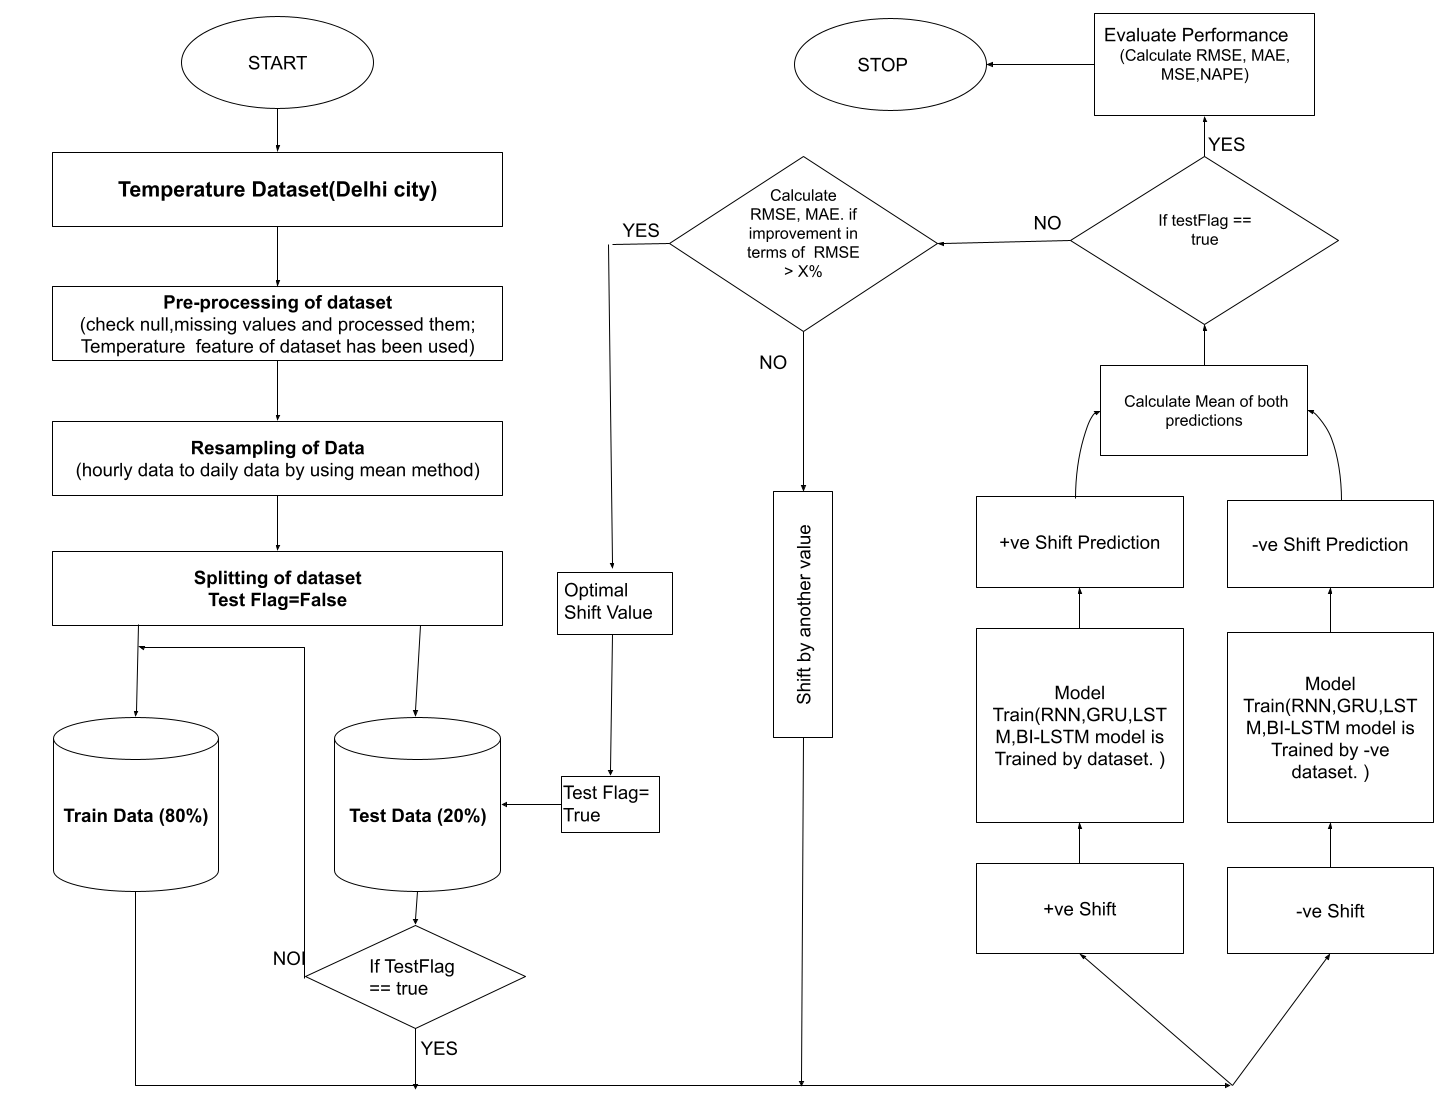
\includegraphics[width=1\textwidth, height=0.9\linewidth]{FlowchartOfjournal.png}
    \caption{Flowchart Of Proposed Work}
    \label{fig:Flowchart Of Proposed Work}
\end{figure}
\subsection{Data collection and preprocessing}
\subsubsection{Raw dataset collection}
The dataset used in this study is publicly accessible on NASA's website (https://power.larc.nasa.gov/data-access-viewer/). The dataset contains 195101 rows in CSV format of temperature and dew point of New Delhi from 02/01/2001 to 06/04/2023 on an hourly frequency. T2M are distinct kind of atmospheric condition. These conditions define the temperature of the atmosphere for each record in the dataset D, shown in equation \ref{eqn:d}.

\begin{equation}
\label{eqn:d}
D=\left \{ x_i, y_i \right \}_{i=1}^{k}
\end{equation}

where, D is denoted as Dataset, \(X_i\) is a Temperature data of hours interval, and \(Y_i\) its corresponding time. k denotes the number of samples in the Dataset. For all \(Y_i\) belongs to Y.

\subsubsection{Data preprocessing}
This technique phase consists of four phases. First, dataset D has been resized into a new dimension of daily basis. The function representing the dimension is omega. shown in equation \ref{eqn:c} also we organised the data by date and time and examined the dataset's non-linearity. Furthermore, temperature(T2M) values between 2001 and 2023 have been chosen from the Resized dataset. Each date from January 2, 2001 to April 6, 2023 is placed in the dependent variable column, and each item in that column of time series data for 22 years (2001-2023) having temperature (T2M) as an independent variable column has been added.

\begin{equation}
\label{eqn:c}
D_{new}=\omega \left ( D, p  \times q \right )
\end{equation}

where, \(D_{new}\) is the preprocessed the dataset D. Here,  p x q  are the new dimension of the Dataset.
\subsubsection{Exploratory data analysis(EDA)}

% \begin{table*}[h!]
%   \caption{statistical summarization of Data set}
%   \label{tab: statistical_data_explore }
%   \begin{tabular}{ll}
%   \hline parameters & Values        \\ \hline
%   count & 195101 \\
% mean  & 25.10    \\
% std   & 21.73     \\
% min   & -999   \\
% 25\%  & 18.70     \\
% 50\%  & 26.46     \\
% 75\%  & 31.98     \\
% max   & 48.79 \\ \hline
%   \end{tabular}
%   \end{table*}
this section explain statistical details about our Delhi temperature dataset. It provides insights into the dataset's size, central tendency, variability, distribution, and range. These statistics serve as a foundational resource for analyzing and interpreting temperature trends in Delhi, supporting various climate-related studies, weather forecasts, and informed decision-making processes.The "count" value of 8,128 indicates the dataset's size, revealing that it bound a substantial number of temperature observations or data points. This size underscores the dataset's richness and the depth of information available for analysis, offering a robust foundation for temperature-related insights.The "mean" temperature of 25.49 degrees serves as the arithmetic average of the dataset. It suggests that, on average, the recorded temperatures in Delhi hover around 25.49 degrees. This central tendency measure offers a crucial point of reference, representing the typical temperature value within the dataset.The "standard deviation" (std) of 7.77 quantifies the degree of temperature variation or dispersion in the data. A higher standard deviation indicates more significant variability in the recorded temperatures. In this case, the standard deviation of 7.77 implies that temperature readings in Delhi can exhibit substantial fluctuations around the mean, signifying the presence of diverse temperature patterns.

The "min" value of 6.95 is the smallest observed temperature in the dataset. However, this value appears unusual and may require further investigation. some previous Values like -999 often signify missing data or anomalies that warrant scrutiny to ensure data quality and integrity so it is handled by taking mean of successor and predecessor value of timeseries dataset .The "max" value of 41.81 denotes the highest temperature recorded in the dataset, offering a glimpse into the upper limit of temperature extremes experienced in Delhi.The quartile values—25\% (first quartile), 50\% (median), and 75\% (third quartile)—offer valuable insights into the distribution of temperatures in Delhi. The first quartile at 18.73 indicates that 25\% of temperature readings fall below this level, while the third quartile at 31.48 signifies that 75\% of the temperatures are below this threshold. The median value of 26.85, which is also the second quartile, represents the middle point of the dataset when arranged in ascending order. Importantly, the median is a robust measure of central tendency that is not affected by extreme outliers. These quartile values provide context for understanding the spread and distribution of temperature data in Delhi.



  \begin{figure}[ht!]
    \centering
    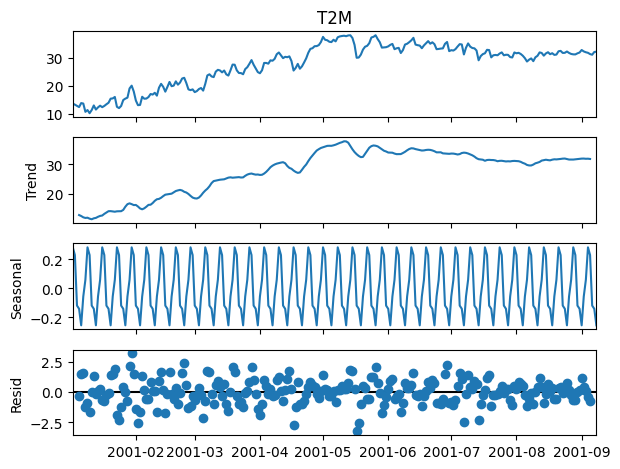
\includegraphics[width=1\textwidth, height=0.75\linewidth]{Graphycal_EDA.png}
    \caption{The Decomposition of data as trend, seasonal and residual of  jan. 2001 to sept. 2001.  }
    \label{fig:graphycalEDA}
\end{figure}
In our dataset, a good trend is visualised. A trend represents a substantial and meaningful long-term pattern in temperature variations. This pattern provide the fundamental direction in which the 2-meter air temperature is changing over an extended period. In climate science, recognizing such trends is vital for understanding the dynamics of temperature variations over time, whether it's the moderate warming associated with climate change or the multi-year temperature cycles linked to climate phenomena like Delhi. Accurately identifying and modeling these trends is pivotal for climate scientists and meteorologists, as it enables them to make informed projections about future temperature changes, prepare for potential impacts, and implement mitigation strategies.
In the context of our temperature dataset, "seasonality" represents the regular and cyclical fluctuations in temperature that occur at consistent intervals throughout the year. These fluctuations often align with the changing of the seasons, resulting in patterns like warmer temperatures during summer and colder temperatures during winter. Seasonality in T2M data can be attributed to various factors, including the tilt of the Earth's axis, which leads to variations in sunlight exposure throughout the year. Identifying seasonality in temperature data is critical for climate scientists and ecologists, as it aids in understanding the impact of changing seasons on ecosystems, agriculture, and human activities. This knowledge is crucial for tasks like crop planning, energy demand forecasting, and environmental conservation efforts.

Residuals in our temperature dataset refer to the unexplained fluctuations or variations that remain after accounting for the identified trends and seasonality. These residuals represent the difference between the observed 2-meter air temperatures and the values predicted by a model that incorporates the long-term trends and seasonal patterns. In climate research, analyzing residuals is vital for assessing the accuracy of climate models and identifying any irregular or unanticipated temperature fluctuations. Residuals should ideally exhibit no systematic patterns; if they do, it suggests that the model may need refinement to better capture the underlying dynamics of temperature changes. Effective handling of residuals is essential for producing reliable temperature predictions, which, in turn, inform climate policy, weather forecasts, and resilience planning in the face of temperature-related challenges.
% \subsection{Train, and Test Splitting of Dataset}



% \par {\textbf{Step 4}: Applying Deep Learning Models:}\\ the model \(\emptyset\left(D_{Tr}\ ,\ D_{Te}\right)\) has been applied. In the model's training and test part, the forecasting has been obtained for the test sample. Prediction is obtained:\(\left\{P_i^\emptyset\right\}_i^m\),  where m is number of test sample %\cite{hrithik2022classification}.

% \par {\textbf{Step 5}: Root Mean Squared Error:}\\ RMSE is calculated by equation \ref{eqn:e}.



% Where N is total no of test Sample, \(\hat{y_{i}}\) is a predicted data of model, and \(y_{i}\) is the actual test deta.\\
% \par {\textbf{Step 6}: Proposed Technique:} \\
\subsection{Proposed model}
\begin{figure}[ht!]
    \centering
    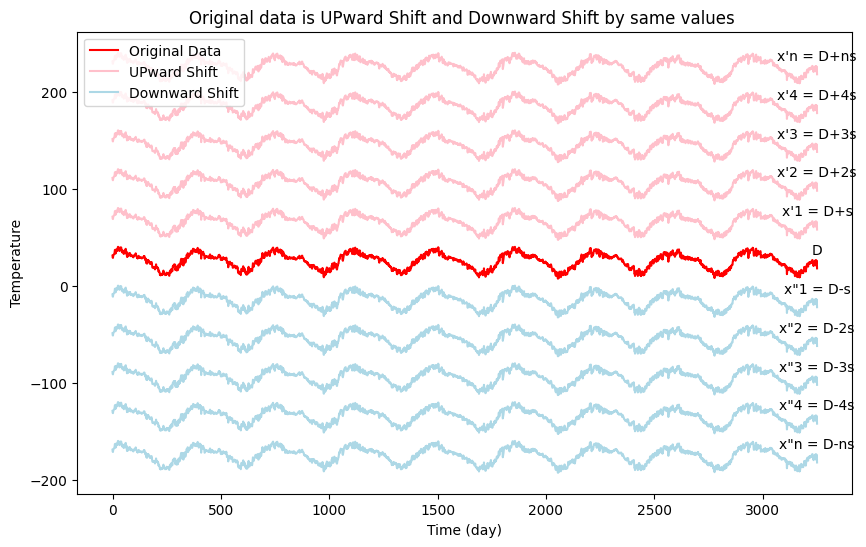
\includegraphics[width=1\textwidth, height=0.9\linewidth]{shifted_dataset.png}
    \caption{Pictorial representation of Multi-Bidirectional shifting based data transformation(MBiS-DT)}
    \label{fig:shifted_dataset}
\end{figure}
 The preprocessed Dataset has been divided into two parts: training \((T_{train})\) (80\%) and testing \((T_{test})\) (20\%). The Dataset is mutually exclusive in equation \ref{eqn:a} and exhaustive in equation \ref{eqn:b}.

\begin{equation}
\label{eqn:a}
D_{Tr}\cup D_{Te}=D_{T}
\end{equation}

\begin{equation}
\label{eqn:b}
\left \{ D_{Tr} \cap D_{Te} \right \}=\varnothing 
\end{equation}

For the data points $x_i$in the training dataset $D_{Tr}$, two series can be created as in equation \ref{eqn:01}:
\begin{equation}
\begin{aligned}
\label{eqn:01}
\{x_i^{\prime}=x_i+s\}_{i=1}^n \\
\{x_i^{\prime\prime}=x_i-s\}_{i=1}^n \; \forall x_i \in D_{Tr}
\end{aligned}
\end{equation}
where $s \in Z$ and $x_i^{\prime}$ and $x_{i}^{\prime\prime}$ depicts the positive and negative series obtained by shifting the series with positive and negative values of the step length $s$ of the shift. The series have been prepared for $n$ number of iterations.
Predictions for both the positive $x_i^{\prime}$and negative $x_i^{\prime\prime}$series has been obtained as $y_i^{\prime}$ and $y_i{\prime\prime}$ respectively.
The predictions are combined to form a final set of predictions using equation \ref{eqn:02} which is utilized for the comparison with the actual values of training dataset $D_{Tr}$
\begin{equation}
\label{eqn:02}
\hat{y}_{final}=\frac{y_i^{\prime}+y_i^{\prime\prime}}{2}
\end{equation}
where $\hat{y}_{final}$ represents the final prediction. The above procedure is repeated for $n$ number of iterations and an optimal value of $s$ is obtained for which the RMSE is best out of $n$ number of iterations. 
Then, the model is trained for the actual training data $D_{Tr}$ and predictions are obtained for the test data $D_{Te}$ which is $D_{Te}^{\prime}$. Further two positive and negative series are obtained from test prediction $D_{Te}^{\prime}$ as reflected in equation \ref{eqn:03}.
\begin{equation}
\begin{aligned}
\label{eqn:03}
\{x_j^{\prime}=x_j+s\} \\
\{x_j^{\prime\prime}=x_j-s\} \; \forall x_j \in D_{Te}^{\prime}
\end{aligned}
\end{equation}
where $s$ is the step length obtained earlier and $x_j^{\prime}$ and $x_{j}^{\prime\prime}$ depicts the positive and negative series obtained by shifting the series with positive and negative values of the step length $s$ of the test predictions $ D_{Te}^{\prime}$.
Predictions for both the positive $x_j^{\prime}$and negative $x_j^{\prime\prime}$series has been obtained as $y_j^{\prime}$ and $y_j{\prime\prime}$ respectively.

The predictions are combined to form a final set of predictions using equation \ref{eqn:04} which is utilized for the comparison with the actual values of training dataset $D_{Te}$
\begin{equation}
\label{eqn:04}
\hat{y}_{final}^{\prime}=\frac{y_j^{\prime}+y_j^{\prime\prime}}{2}
\end{equation}
where $\hat{y}_{final}^{\prime}$ represents the final prediction.


\begin{figure}[ht!]
%\centering
\subfloat[Test data vs Proposed MBiS-DT GRU] {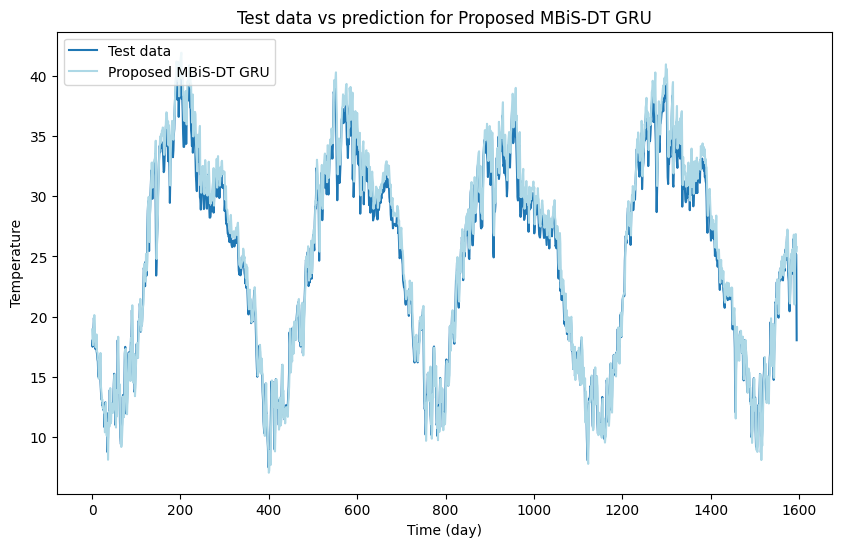
\includegraphics[scale=0.3]{testData_vs_proposed_GRU.png}\label{fig:BarPlot_TestDataVSMBiS-DT_GRU}}
\hfill
\subfloat[Test data vs Proposed MBiS-DT RNN]{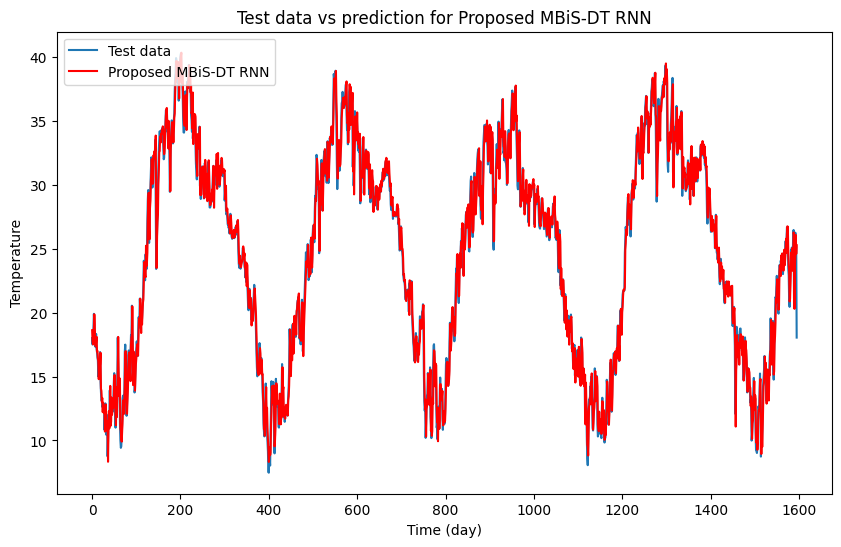
\includegraphics[scale=0.3]{testData_vs_proposed_RNN.png}\label{fig:BarPlot_TestDataVSMBiS-DT_RNN}}\\
\subfloat[Test data vs Proposed MBiS-DT BI-LSTM]{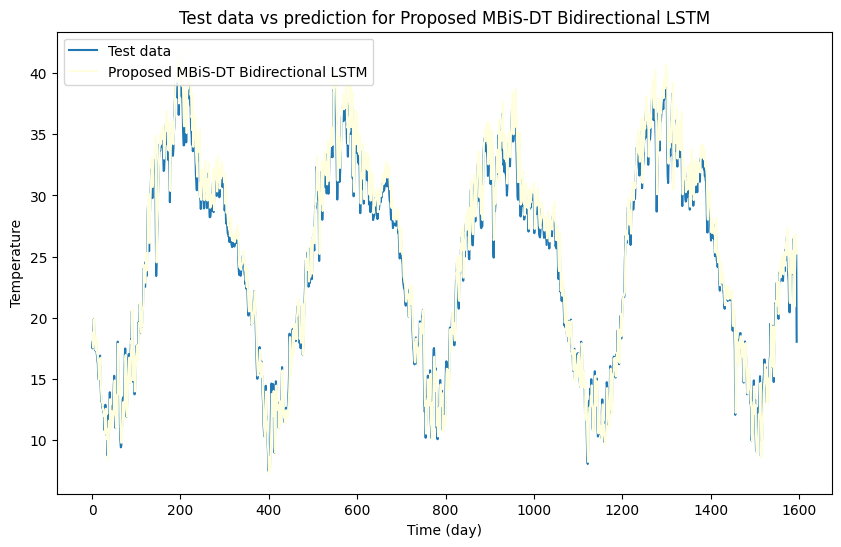
\includegraphics[scale=0.3]{testData_vs_proposed_BI-lstm.png}\label{fig:BarPlot_TestDataVSMBiS-DT_BILSTM}}
\hfill
\subfloat[Test data vs Proposed MBiS-DT LSTM]{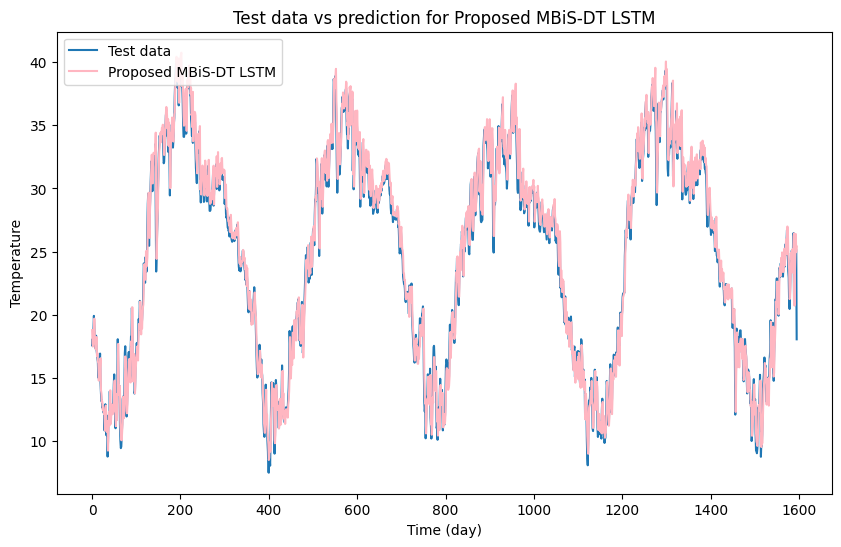
\includegraphics[scale=0.3]{testData_vs_proposed_LSTM.png}\label{fig:BarPlot_TestDataVSMBiS-DT_LSTM}}
  \caption{Line plot of vs proposed MBiS-DT models}
  \label{fig:Line plot of vs proposed MBiS-DT models}
\end{figure} 


% \begin{figure}[ht!]
%     \centering
%     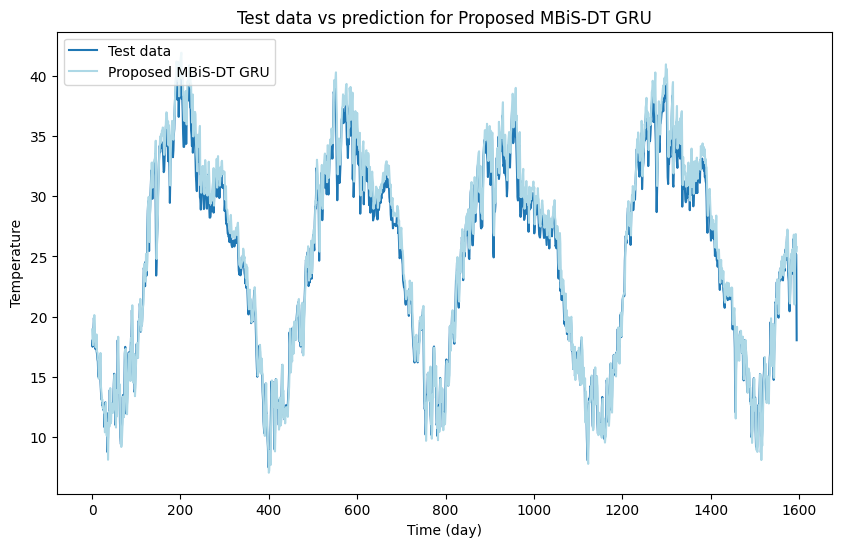
\includegraphics[width=1\textwidth, height=0.9\linewidth]{testData_vs_proposed_GRU.png}
%     \caption{Test data vs Proposed MBiS-DT GRU}
%     \label{fig:BarPlot_TestDataVSMBiS-DT_GRU}
% \end{figure}
% \begin{figure}[ht!]
%     \centering
%     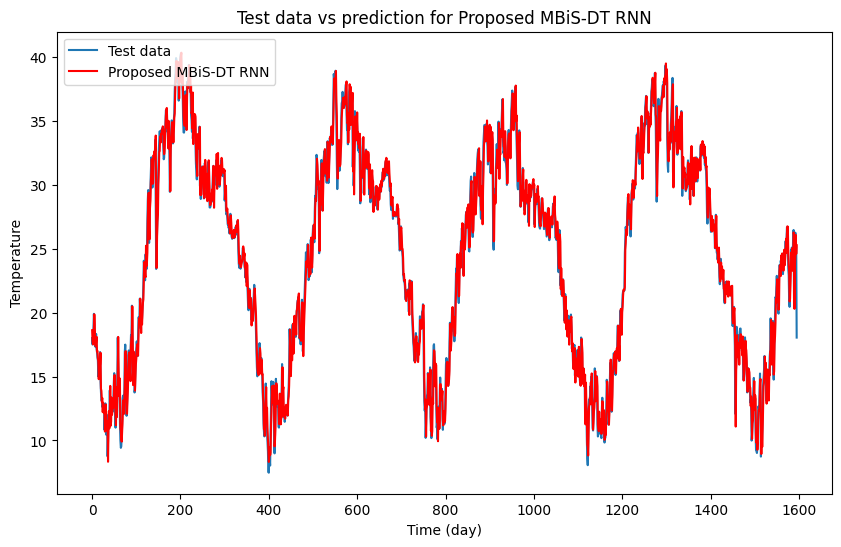
\includegraphics[width=1\textwidth, height=0.9\linewidth]{testData_vs_proposed_RNN.png}
%     \caption{Test data vs Proposed MBiS-DT RNN}
%     \label{fig:BarPlot_TestDataVSMBiS-DT_RNN}
% \end{figure}
% \begin{figure}[ht!]
%     \centering
%     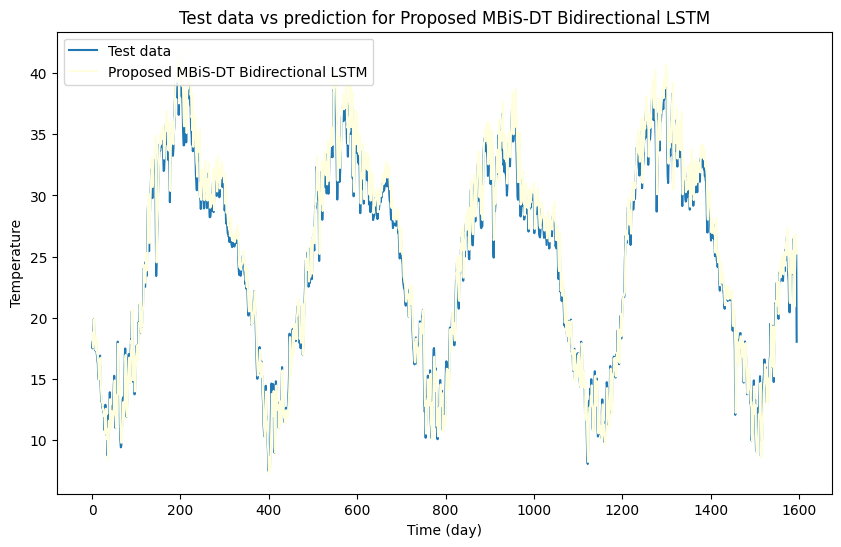
\includegraphics[width=1\textwidth, height=0.9\linewidth]{testData_vs_proposed_BI-lstm.png}
%     \caption{Test data vs Proposed MBiS-DT BI-LSTM}
%     \label{fig:BarPlot_TestDataVSMBiS-DT_BILSTM}
% \end{figure}
% \begin{figure}[ht!]
%     \centering
%     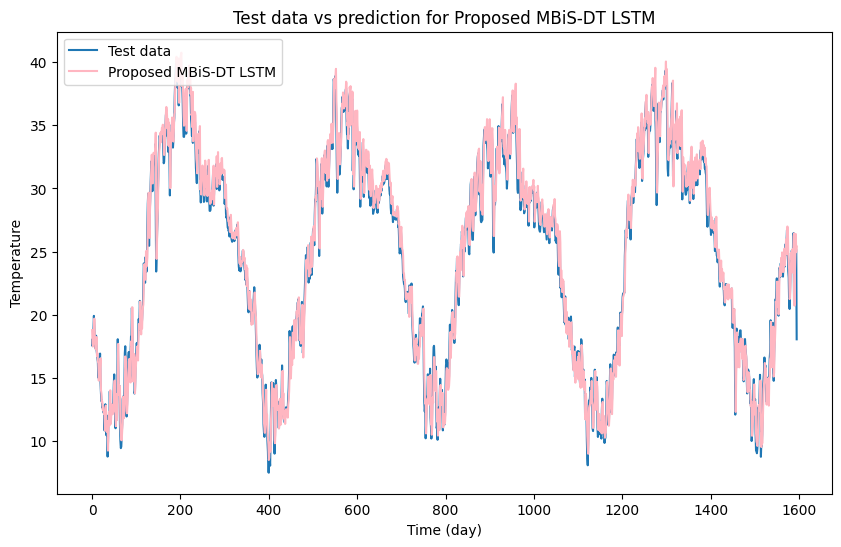
\includegraphics[width=1\textwidth, height=0.9\linewidth]{testData_vs_proposed_LSTM.png}
%     \caption{Test data vs Proposed MBiS-DT LSTM}
%     \label{fig:BarPlot_TestDataVSMBiS-DT_LSTM}
% \end{figure}





\begin{figure}[ht!]
  %\centering
  \subfloat[Test data vs Proposed MBiS-DT GRU] {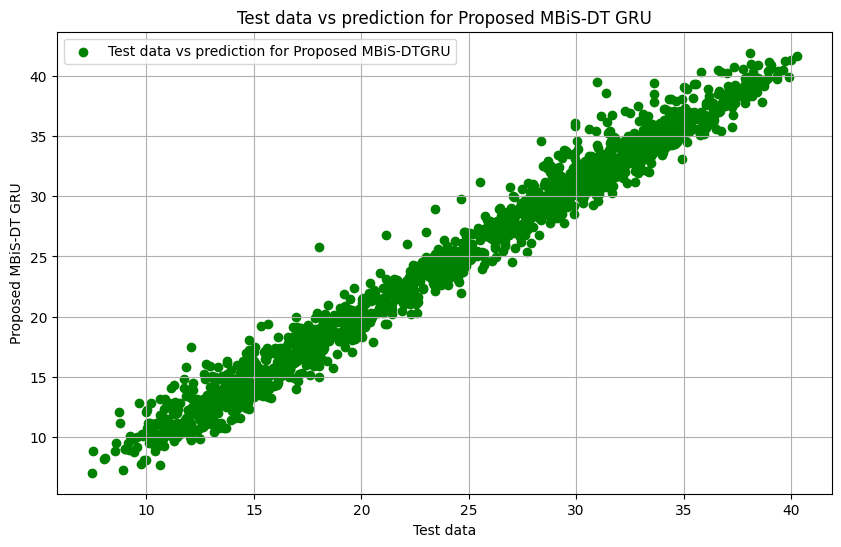
\includegraphics[scale=0.3]{scatter_gru.png}\label{fig:ScatterPlot_TestDataVSMBiS-DT_GRU}}
  \hfill
  \subfloat[Test data vs Proposed MBiS-DT RNN]{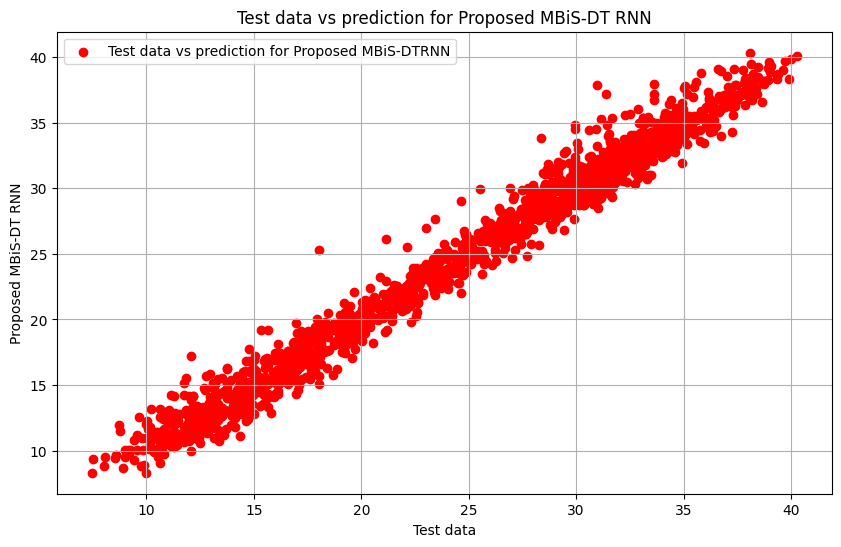
\includegraphics[scale=0.3]{scatter_rnn.png}\label{fig:ScatterPlot_TestDataVSMBiS-DT_RNN}}\\
  \subfloat[Test data vs Proposed MBiS-DT BI-LSTM]{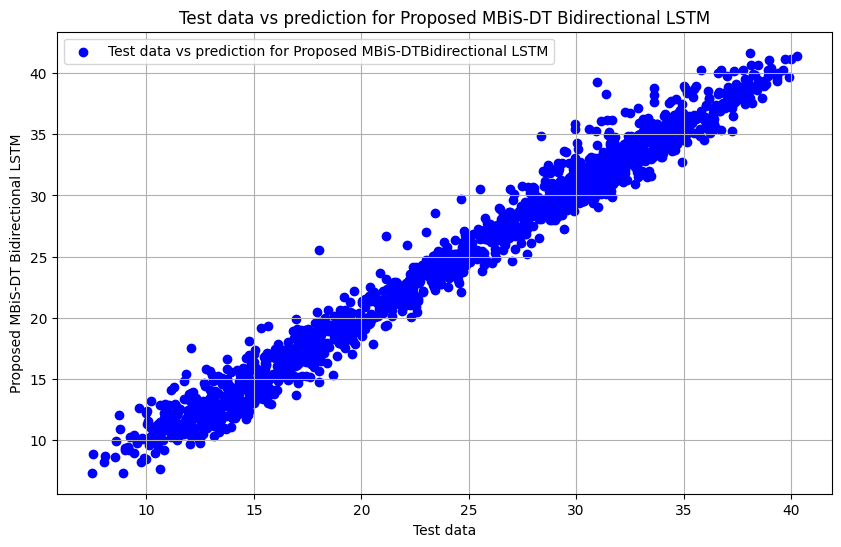
\includegraphics[scale=0.3]{scatter_bilstm.png}\label{fig:ScatterPlot_TestDataVSMBiS-DT_BI-LSTM}}
  \hfill
  \subfloat[Test data vs Proposed MBiS-DT LSTM]{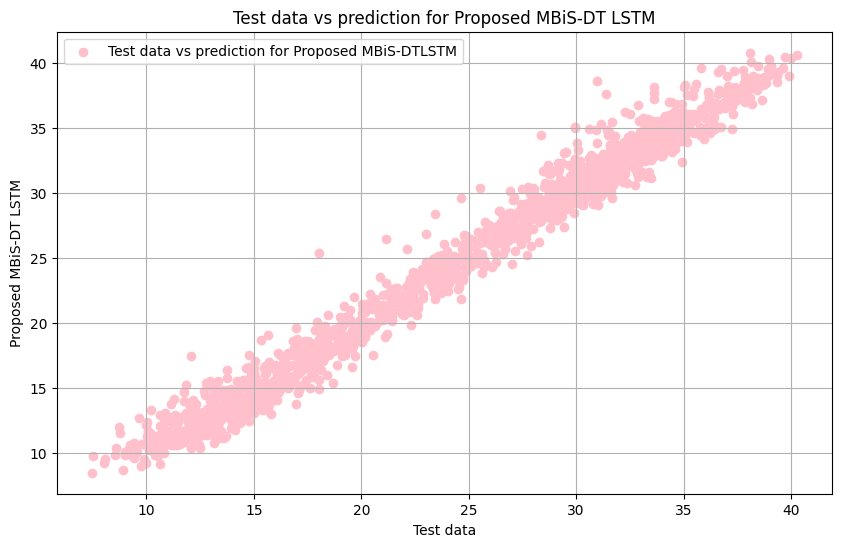
\includegraphics[scale=0.3]{scatter_lstm.png}\label{fig:ScatterPlot_TestDataVSMBiS-DT_LSTM}}
    \caption{Scatter plot of vs proposed MBiS-DT models}
    \label{fig:Scatter plot of vs proposed MBiS-DT models}
  \end{figure}




% \begin{figure}[ht!]
%     \centering
%     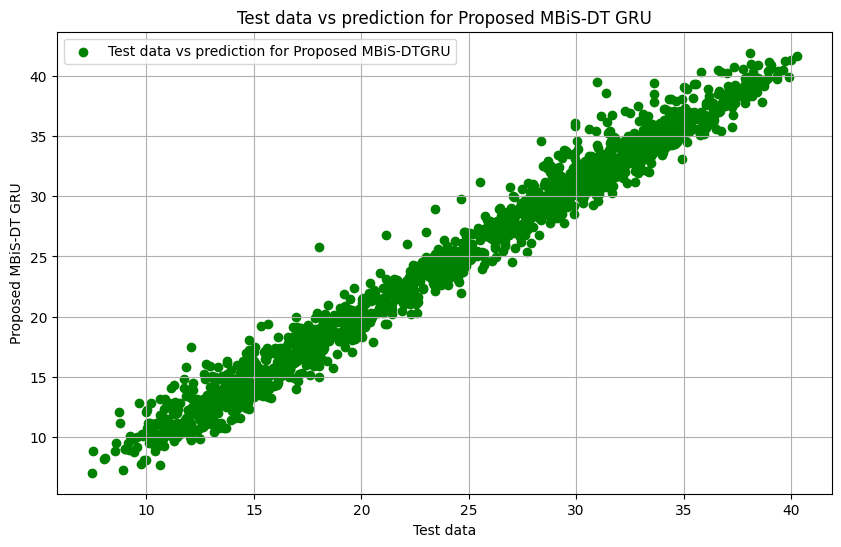
\includegraphics[width=1\textwidth, height=0.9\linewidth]{scatter_gru.png}
%     \caption{Test data vs Proposed MBiS-DT GRU}
%     \label{fig:ScatterPlot_TestDataVSMBiS-DT_GRU}
% \end{figure}
% \begin{figure}[ht!]
%     \centering
%     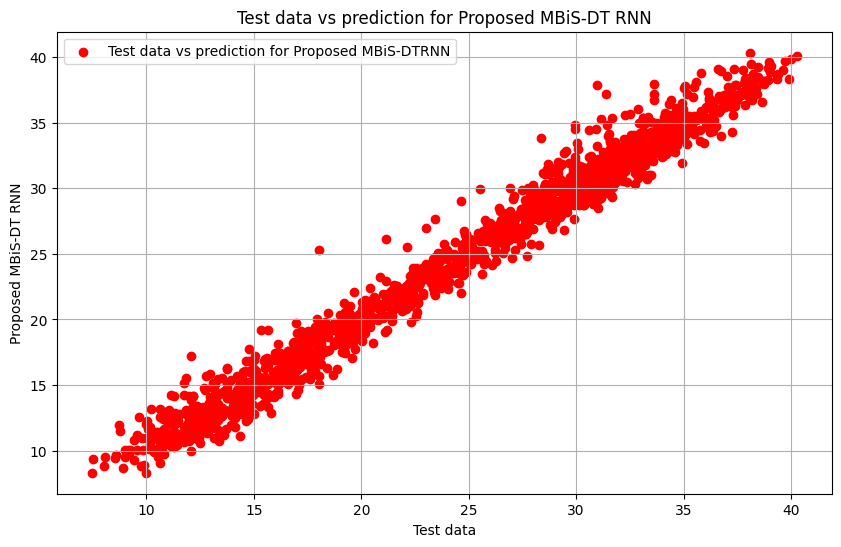
\includegraphics[width=1\textwidth, height=0.9\linewidth]{scatter_rnn.png}
%     \caption{Test data vs Proposed MBiS-DT RNN}
%     \label{fig:ScatterPlot_TestDataVSMBiS-DT_RNN}
% \end{figure}
% \begin{figure}[ht!]
%     \centering
%     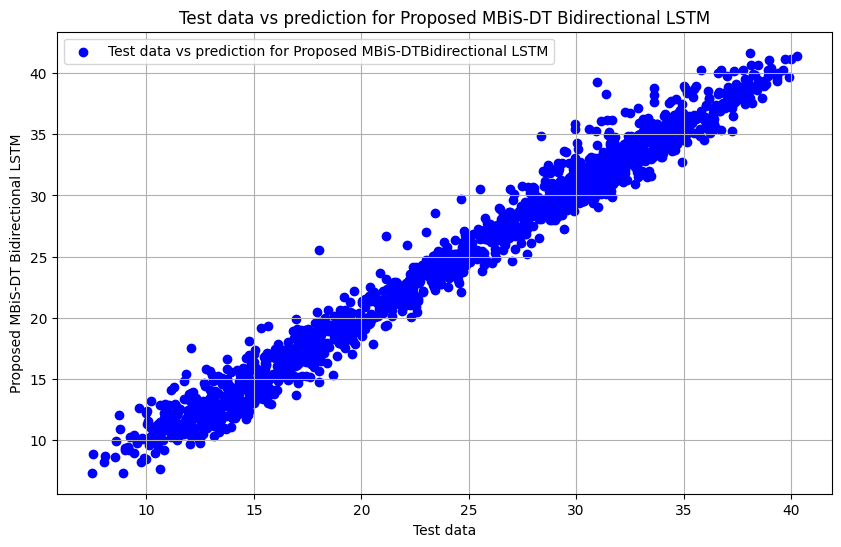
\includegraphics[width=1\textwidth, height=0.9\linewidth]{scatter_bilstm.png}
%     \caption{Test data vs Proposed MBiS-DT BI-LSTM}
%     \label{fig:ScatterPlot_TestDataVSMBiS-DT_BI-LSTM}
% \end{figure}
% \begin{figure}[ht!]
%     \centering
%     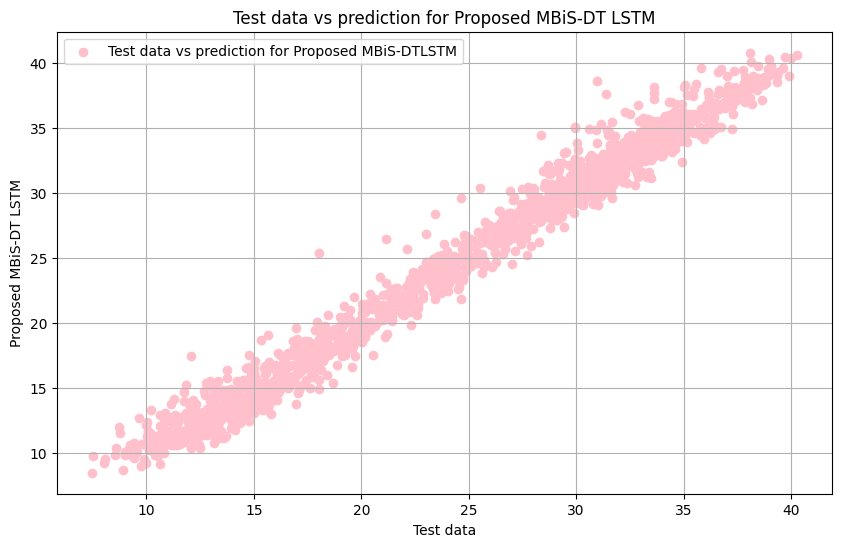
\includegraphics[width=1\textwidth, height=0.9\linewidth]{scatter_lstm.png}
%     \caption{Test data vs Proposed MBiS-DT LSTM}
%     \label{fig:ScatterPlot_TestDataVSMBiS-DT_LSTM}
% \end{figure}




\subsection{Performance Measures:}
\subsubsection{Root Mean Squared Error (RMSE)}:
This performance metric is used widely in regression tasks, including temperature prediction. It calculates the average magnitude of the errors between actual and predicted values. RMSE is calculated by taking the square root of the average of the squared differences between actual and predicted values.

The formula for RMSE is as in equation \ref{eqn:e}:
\begin{equation}
\label{eqn:e}
RMSE = \sqrt {\frac{1}{N} \sum_{i=1}^{N} (\hat{y_{i}} - y_{i})^2}
\end{equation}
Where the variables $\hat{y}_i$ is predicted values of the target variable (e.g., temperature), $y_i$ is the Actual values of the target variable and N is the total number of data point in the dataset.
\subsubsection{Mean Absolute Error (MAE):} It is a data dependent performance metric used for evaluation of average of exact error between actual and predicted variables. The formula for MAE is depicted in equation \ref{eqn:mae}
\begin{equation}
\label{eqn:mae}
MAE = \frac{1}{N} \sum_{i=1}^{N} \mid\hat{y_{i}} - y_{i}\mid .
\end{equation}
Where the variables $\hat{y}_i$ is predicted values of the target variable (e.g., temperature), $y_i$ is the Actual values of the target variable and N is the total no. of the data point in dataset.

\subsubsection{Mean Squared Error (MSE):}
Mean Squared Error (MSE) is another widely used performance metric in regression tasks, including temperature prediction. It compute the Mean of the squared differences between actual values and predicted values. MSE emphasizes larger errors value more than smaller errors value due to the squaring of the differences.
The formula for MSE is as depicted in equation \ref{eqn:mse}
\begin{equation}
\label{eqn:mse}
MSE = \frac{1}{N} \sum_{i=1}^{N} (\hat{y_{i}} - y_{i})^2
\end{equation}
Where the variables $\hat{y}_i$ is predicted values of the target variable (e.g., temperature), $y_i$ is the Actual values of the target variable and N is the number of data points in the dataset.


\subsubsection{Mean Absolute Percentage Error (MAPE):}
Mean Absolute Percentage Error (MAPE) is a performance metric commonly used in regression tasks, including temperature prediction. It measures the average percentage difference between predicted and actual values, providing a relative measure of the accuracy of the model's predictions.

The formula for MAPE is represented in equation \ref{eqn:mape}
\begin{equation}
\label{eqn:mape}
MAPE = \frac{100}{N} \sum_{i=1}^{N} \mid(\frac{\hat{y_{i}} - y_{i}}{y_i})\mid .
\end{equation}

%MAPE = (1/n) * Σ(|(y_actual - y_pred) / y_actual|) * 100

Where the variables $\hat{y}_i$ is predicted values of the target variable (e.g., temperature), $y_i$ is the Actual values of the target variable and N is the number of data points in the dataset.



\subsection{Implamentation setup and parameters settings}
The various packages of Python are utilised to implement the baseline models and  proposed models. These include Pandas (v1.5.3), Scikit-Learn (v1.2.2) for model creation and performance analysis, Keras (v2.12.0), TensorFlow (v2.12.0) for Keras backend, and NumPy (v1.23.5) for exploratory data analysis,  and For describing the findings and creating graphs, we used Plotly (v5.14.1), seaborn (v0.12.2), and matplotlib (v3.7.1). In order to create flowcharts, it has also used \href{https: //app.diagrams.net/}{https: //app.diagrams.net/} . One systems were employed for the experiments:  a MacOS-based computer with Apple M1 having 8 GB RAM. and all exprement done on Google colab having runtime type Python 3 and hardware accelerate T4 GPU with 12.7Gb Ram.

\begin{table*}[h!]
\centering
  \caption{Parameter setting of traditional DL models and proposed MBiS-DT Models}
  \label{tab: my-table}
  \begin{tabular}{ll}
  \hline Hyperparameters & Values        \\ \hline
  Batch Size               & 32                     \\
  Optimizer                 & Adam                   \\
  Loss function            & Mean Squared Error      \\
  Epoch                    & 200 with early stopping \\
  training size             & 0.8                   \\ \hline
  \end{tabular}
  \end{table*}

\section{Results and discussion}\label{sec2}
The percentage improvement  of the experimented models namely LSTM, GRU, BiLSTM and RNN has been depicted in Table \ref{tab:MSE} on the basis of MSE. The maximum improvement achieved is of 47.33 \% in case of GRU where the shift length is kept as 35. Other models also show significant improvement after the implementation of proposed methodology.
% \begin{table}[ht!]
% \centering
% \caption{MSE}
% \label{tab:MSE}
% \begin{tabular}{lllll}
% \hline
% \textbf{MODELS} & \textbf{ORIGINAL} & \textbf{\% IMPROVEMENT} & \textbf{PROPOSED (P)} & \textbf{SHIFT LENGTH} \\ \hline
% \textbf{LSTM}    & 1.97   & 19.54 & 1.59 & 20 \\
% \textbf{GRU}     & 3.35 & 47.73 & 1.75 & 35 \\
% \textbf{BI-LSTM} & 1.62   & 15.86 & 1.36 & 35 \\
% \textbf{RNN}     & 1.94   & 21.37 & 1.52 & 35 \\ \hline
% \end{tabular}
% \end{table}

\begin{table}[ht!]
\centering
\caption{Performance of different DL models and proposed MBiS-DT models along \% improvement based on Proposed MBiS-DT-BI-LSTM }
\label{tab:MSE}
\begin{tabular}{p{0.1\textwidth}lllllllll}
\hline
\textbf{MODELS} & \textbf{MSE} & \textbf{\% Imp.} & \textbf{RMSE} & \textbf{\% Imp} & \textbf{MAE} & \textbf{\% Imp} & \textbf{MAPE} & \textbf{\% Imp}  \\ \hline
  LSTM    & 1.97 &30.96  & 1.39  &16.54  & 1.07 &16.82  & 4.33 &4.61  \\
  GRU    & 3.35 &59.40  & 1.78 &34.83  & 1.45 & 38.62 & 4.53 &8.83  \\
  BI-LSTM & 1.62   &16.04  & 1.26 &7.93  & 0.99 &10.10  & 4.41 &6.34   \\
  RNN     & 1.94   &29.89  & 1.38 &15.94  & 1.09 &18.34  & 4.95&16.56   \\
\textbf{Proposed MBiS-DT-LSTM}    & \textbf{1.59}  &14.46      & \textbf{1.25} &7.20     & \textbf{0.95} &6.31     & \textbf{4.36} &5.27     \\
\textbf{Proposed MBiS-DT-GRU}     & \textbf{1.75} &22.28     & \textbf{1.31} &11.45     & \textbf{1.03} & 13.59    & \textbf{4.26} &3.05      \\
\textbf{Proposed MBiS-DT-RNN}     & \textbf{1.52}   &10.52     & \textbf{1.23} &5.69     & \textbf{0.97} &8.24     & \textbf{4.55} &9.23     \\
\textbf{Proposed MBiS-DT-BI-LSTM} & \textbf{1.36}   & -    & \textbf{1.16} &-     & \textbf{0.89} & -    & \textbf{4.13} & -     \\
\hline
\end{tabular}
\end{table}


% \begin{table}[ht!]
% \centering
% \caption{MAPE}
% \label{tab:MAPE}
% \begin{tabular}{lllll}
% \hline
% \textbf{MODELS} & \textbf{ORIGINAL} & \textbf{\% IMPROVEMENT} & \textbf{PROPOSED (P)} & \textbf{SHIFT LENGTH} \\ \hline
% \textbf{LSTM}    & 4.33   & -7.78 & 4.36 & 20 \\
% \textbf{GRU}     & 4.53 & 6.10 & 4.26 & 35 \\
% \textbf{BI-LSTM} & 4.41   & 6.31 & 4.13 & 35 \\
% \textbf{RNN}     & 4.95   & 8.10 & 4.55 & 35 \\ \hline
% \end{tabular}
% \end{table}

% \begin{table}[ht!]
% \centering
% \caption{RMSE}
% \label{tab:RMSE}
% \begin{tabular}{lllll}
% \hline
% \textbf{MODELS} & \textbf{ORIGINAL} & \textbf{\% IMPROVEMENT} & \textbf{PROPOSED (P)} & \textbf{SHIFT LENGTH} \\ \hline
% \textbf{LSTM}    & 1.39 & 10.0381 & 1.2593 & 20 \\
% \textbf{GRU}     & 1.78 & 25.98   & 1.31   & 35 \\
% \textbf{BI-LSTM} & 1.26 & 7.99    & 1.16   & 35 \\
% \textbf{RNN}     & 1.38 & 10.38   & 1.2343 & 35 \\ \hline
% \end{tabular}
% \end{table}
% \begin{table}[ht!]
% \centering
% \caption{MAE}
% \label{tab:MAE}
% \begin{tabular}{lllll}
% \hline
% \textbf{MODELS} & \textbf{ORIGINAL} & \textbf{\% IMPROVEMENT} & \textbf{PROPOSED (P)} & \textbf{SHIFT LENGTH} \\ \hline
% \textbf{LSTM}    & 1.07 & 11.20 & 0.95 & 20 \\
% \textbf{GRU}     & 1.45 & 28.8  & 1.03 & 35 \\
% \textbf{BI-LSTM} & 0.99 & 10.10 & 0.89 & 35 \\
% \textbf{RNN}     & 1.09 & 11.24 & 0.97 & 35 \\ \hline
% \end{tabular}
% \end{table}
Figure \ref{fig:all_models_measures} illustrates the comparison of the all experimented models with the performance of the proposed method. 
\\
\begin{figure}[ht!]
%\centering
\subfloat[LSTM Vs Proposed LSTM] {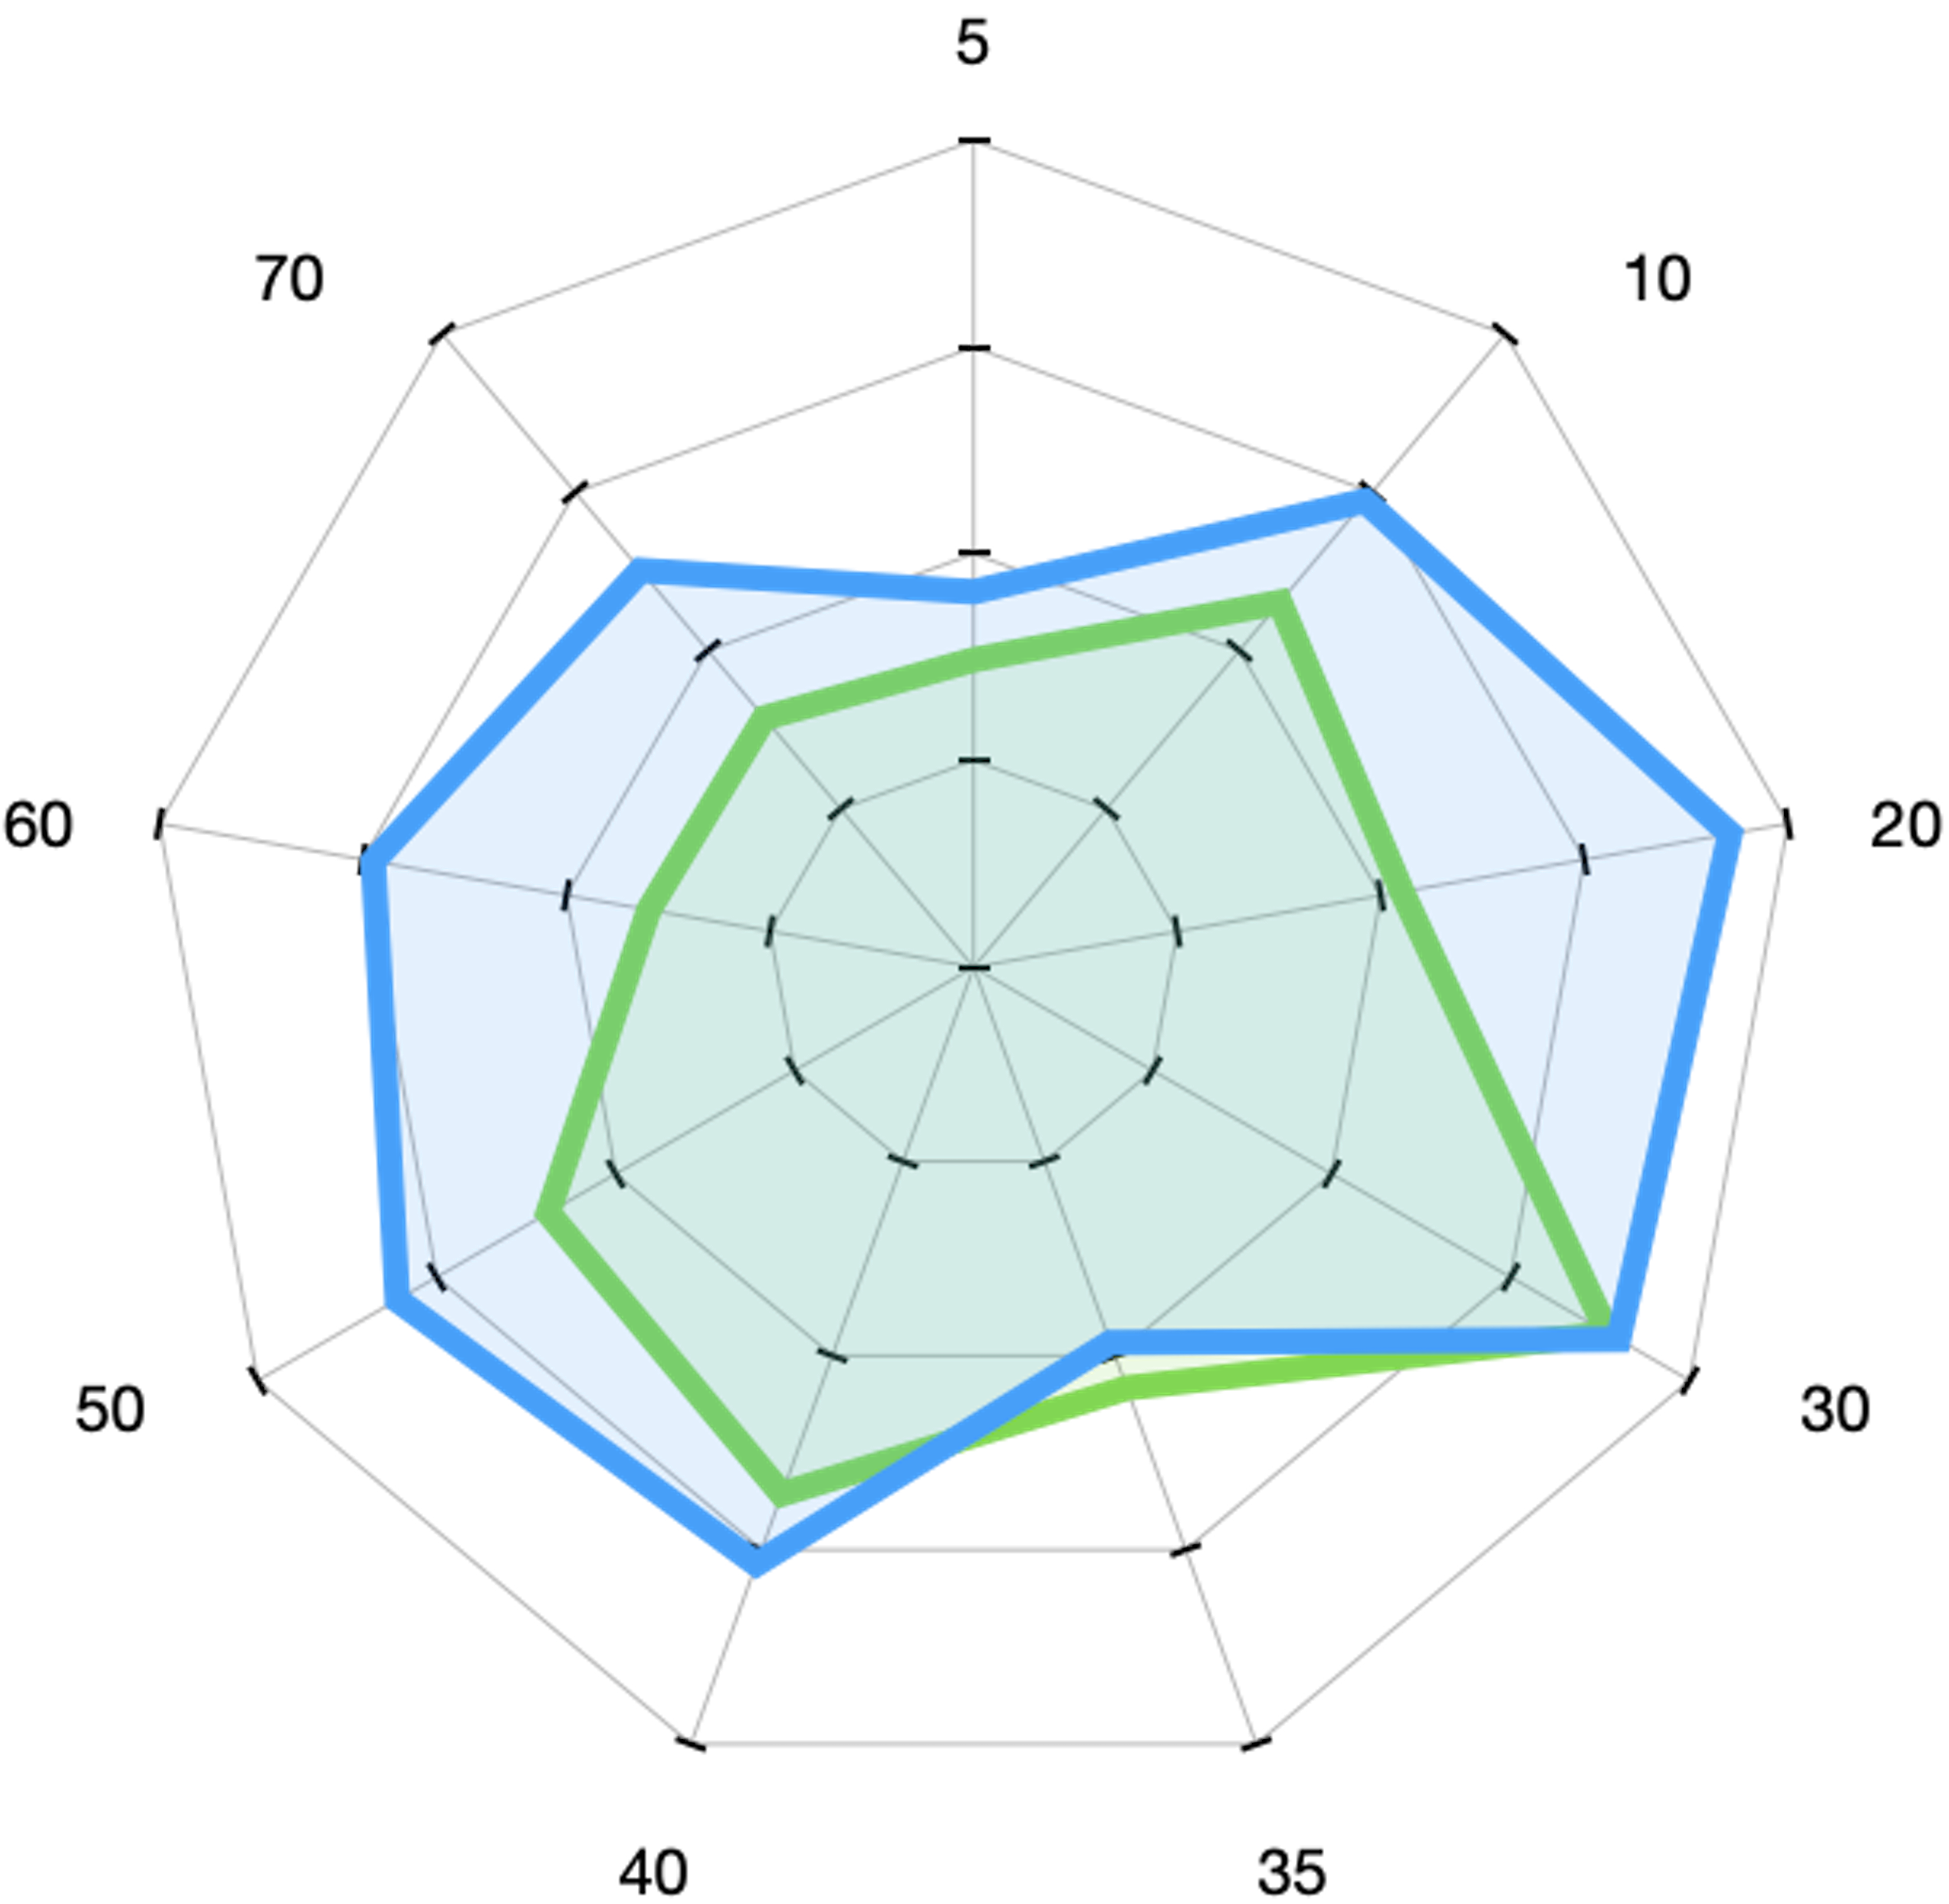
\includegraphics[width=0.4\textwidth, height=0.25\linewidth]{LSTM_MAE_SPIDER.png}\label{fig:LSTM MAE SPIDER}}
\hfill
\subfloat[RNN Vs Proposed RNN]{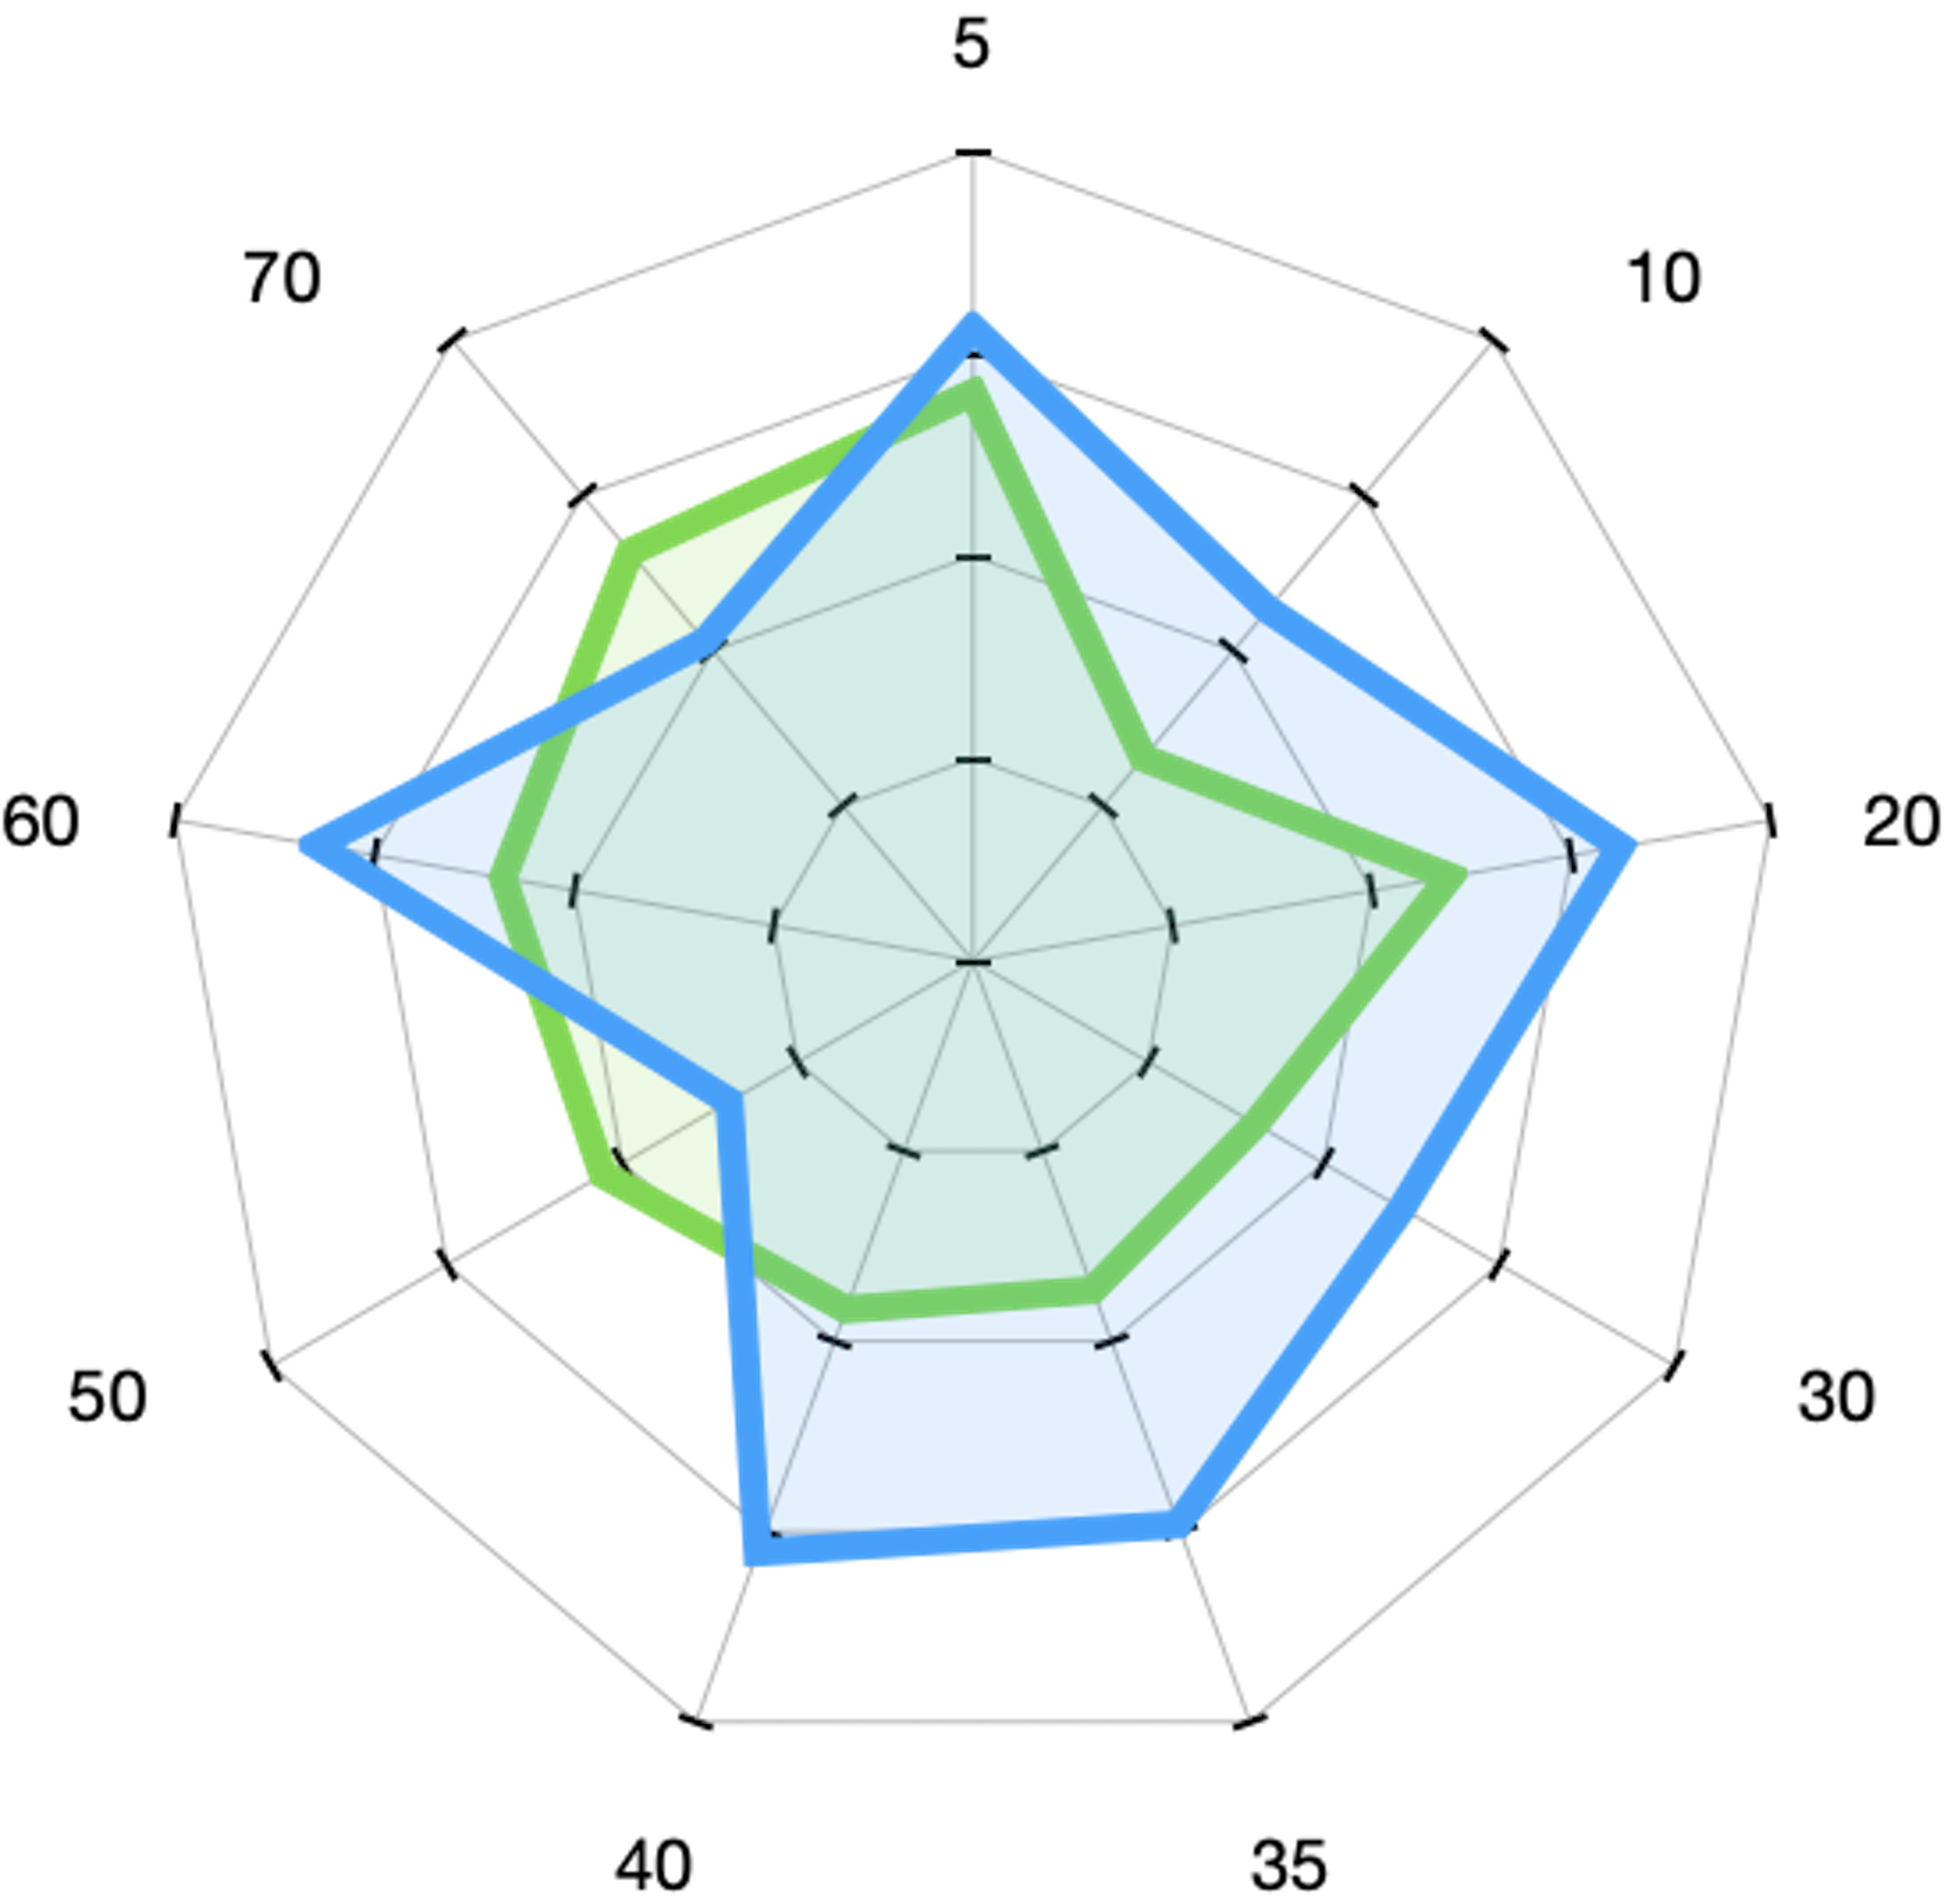
\includegraphics[width=0.4\textwidth, height=0.25\linewidth]{RNN_MAE_SPIDER.png}\label{fig:RNN_MAE_SPIDER}}\\
\subfloat[BiLSTM Vs Proposed RNN]{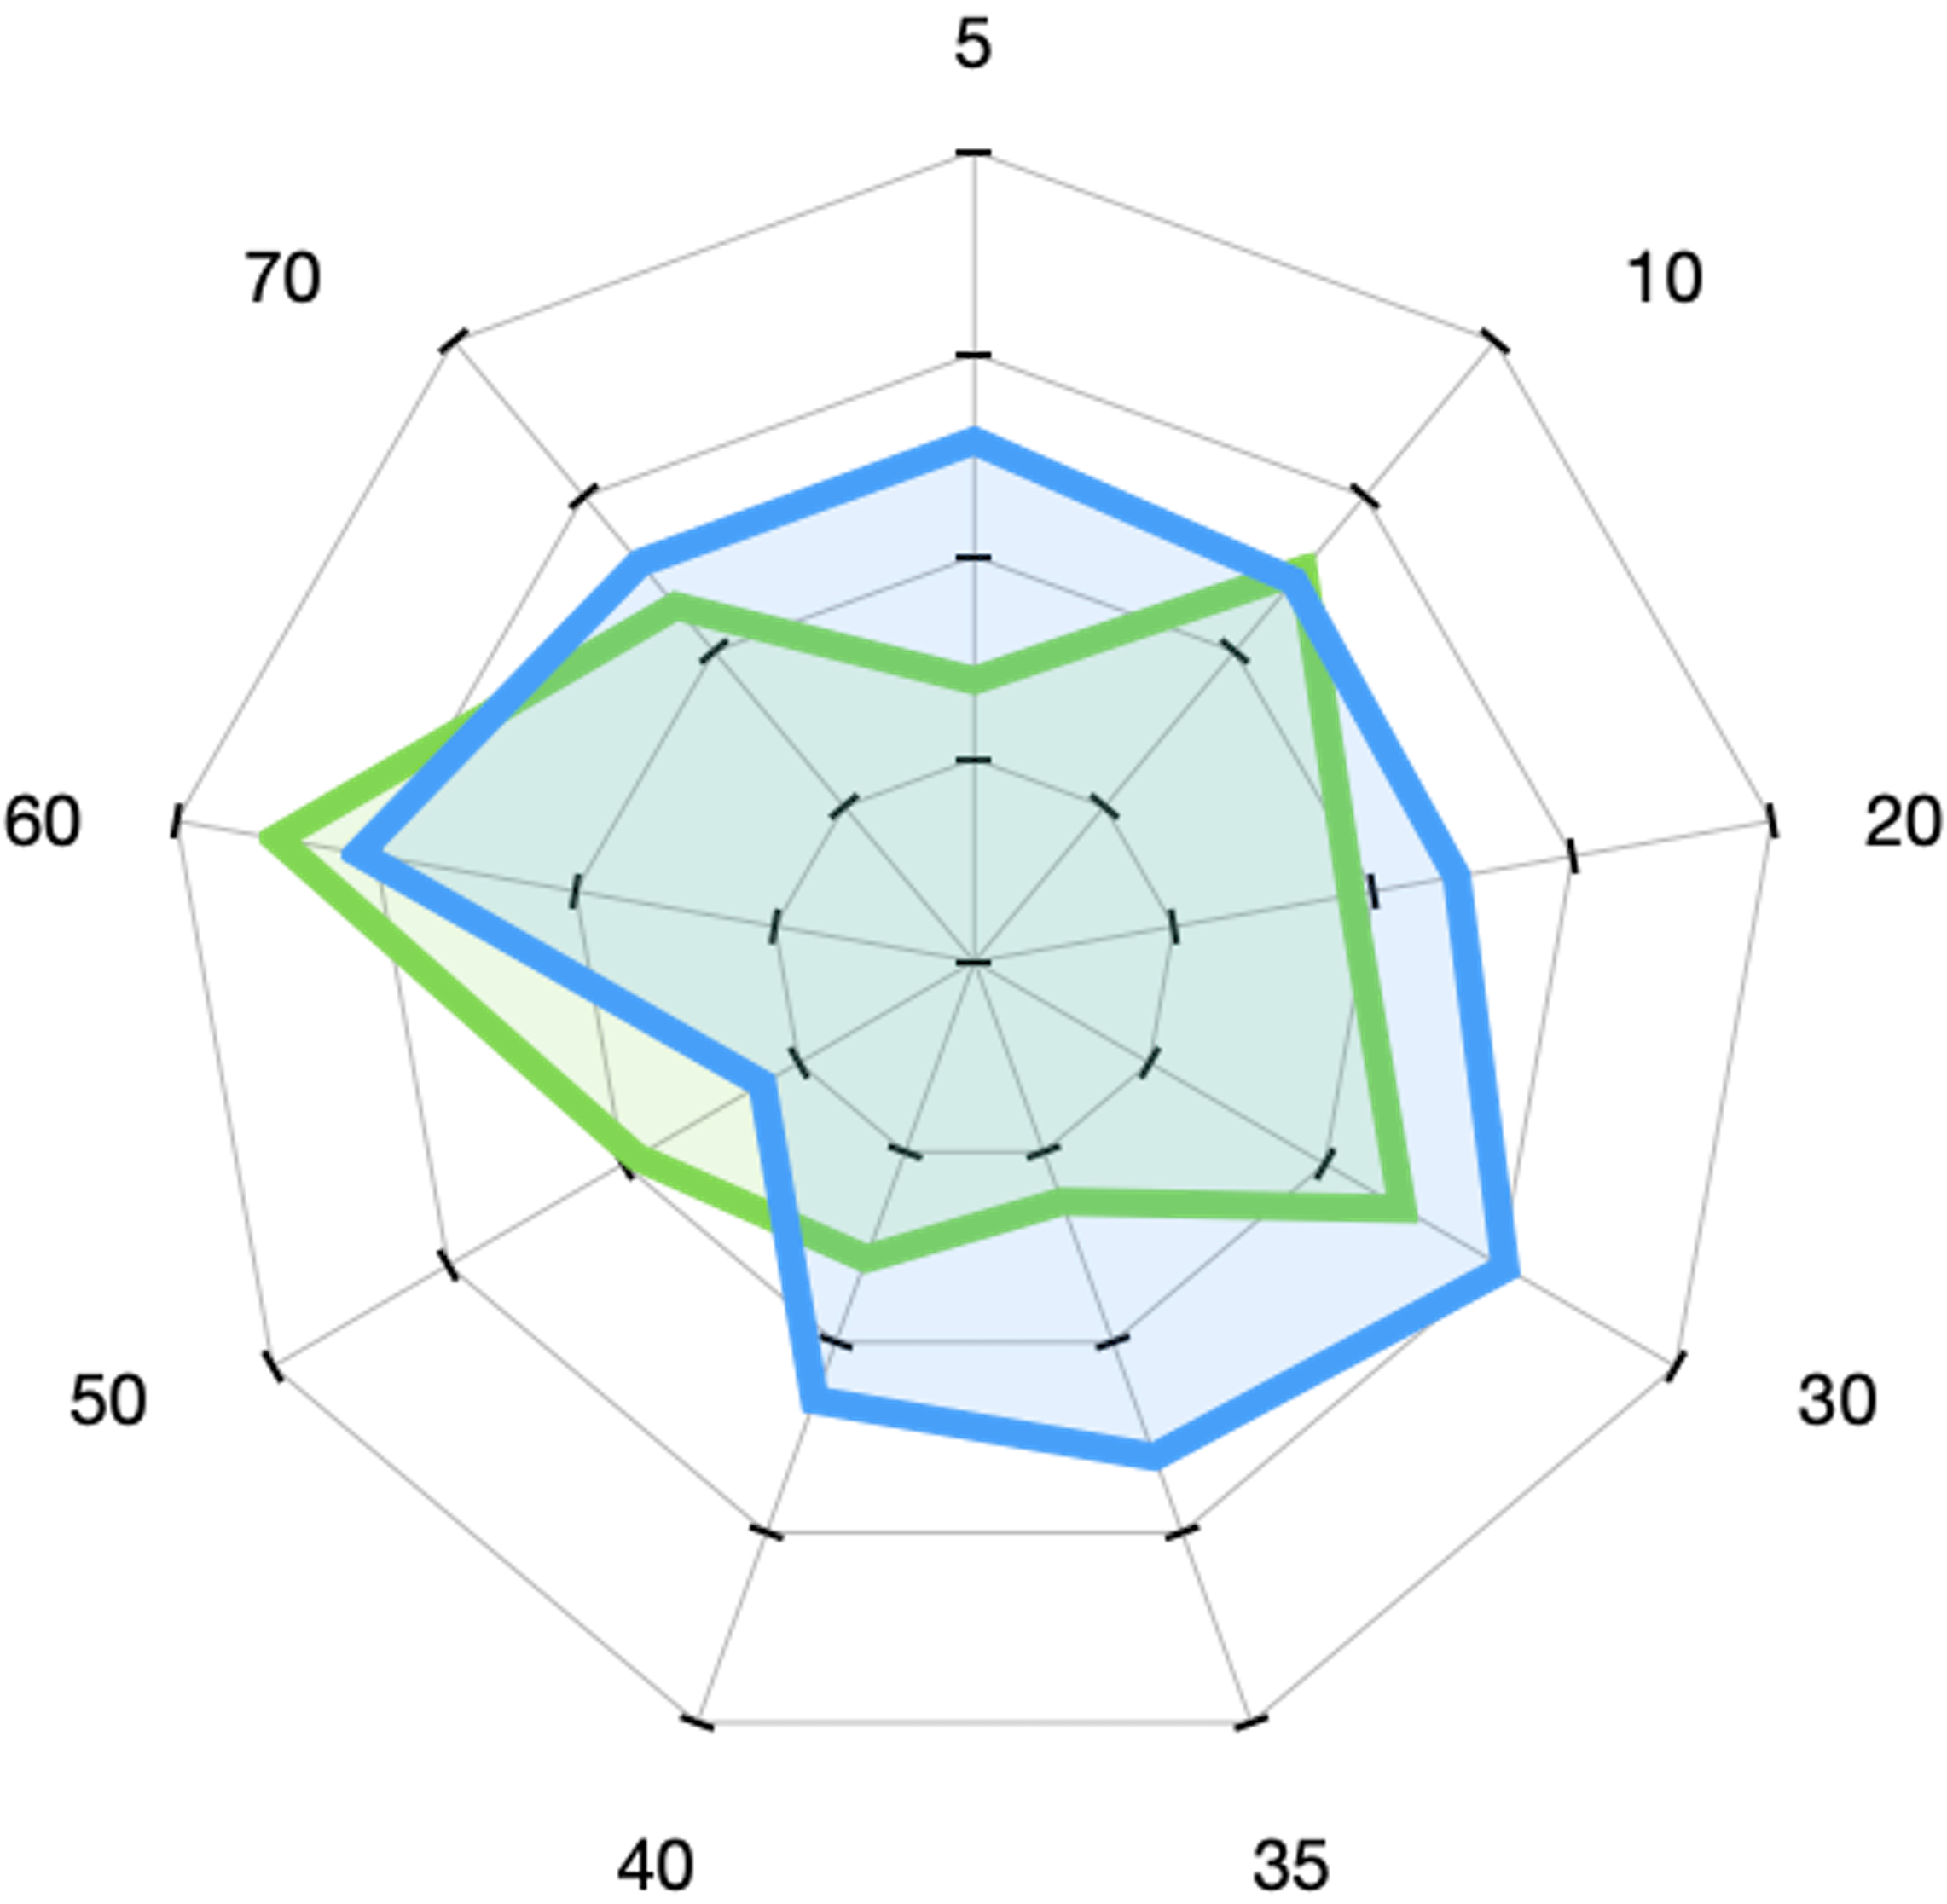
\includegraphics[width=0.4\textwidth, height=0.25\linewidth]{BI-LSTM_MAE_SPIDER.png}\label{fig:BiLSTM_MAE_SPIDER}}
\hfill
\subfloat[GRU Vs Proposed GRU]{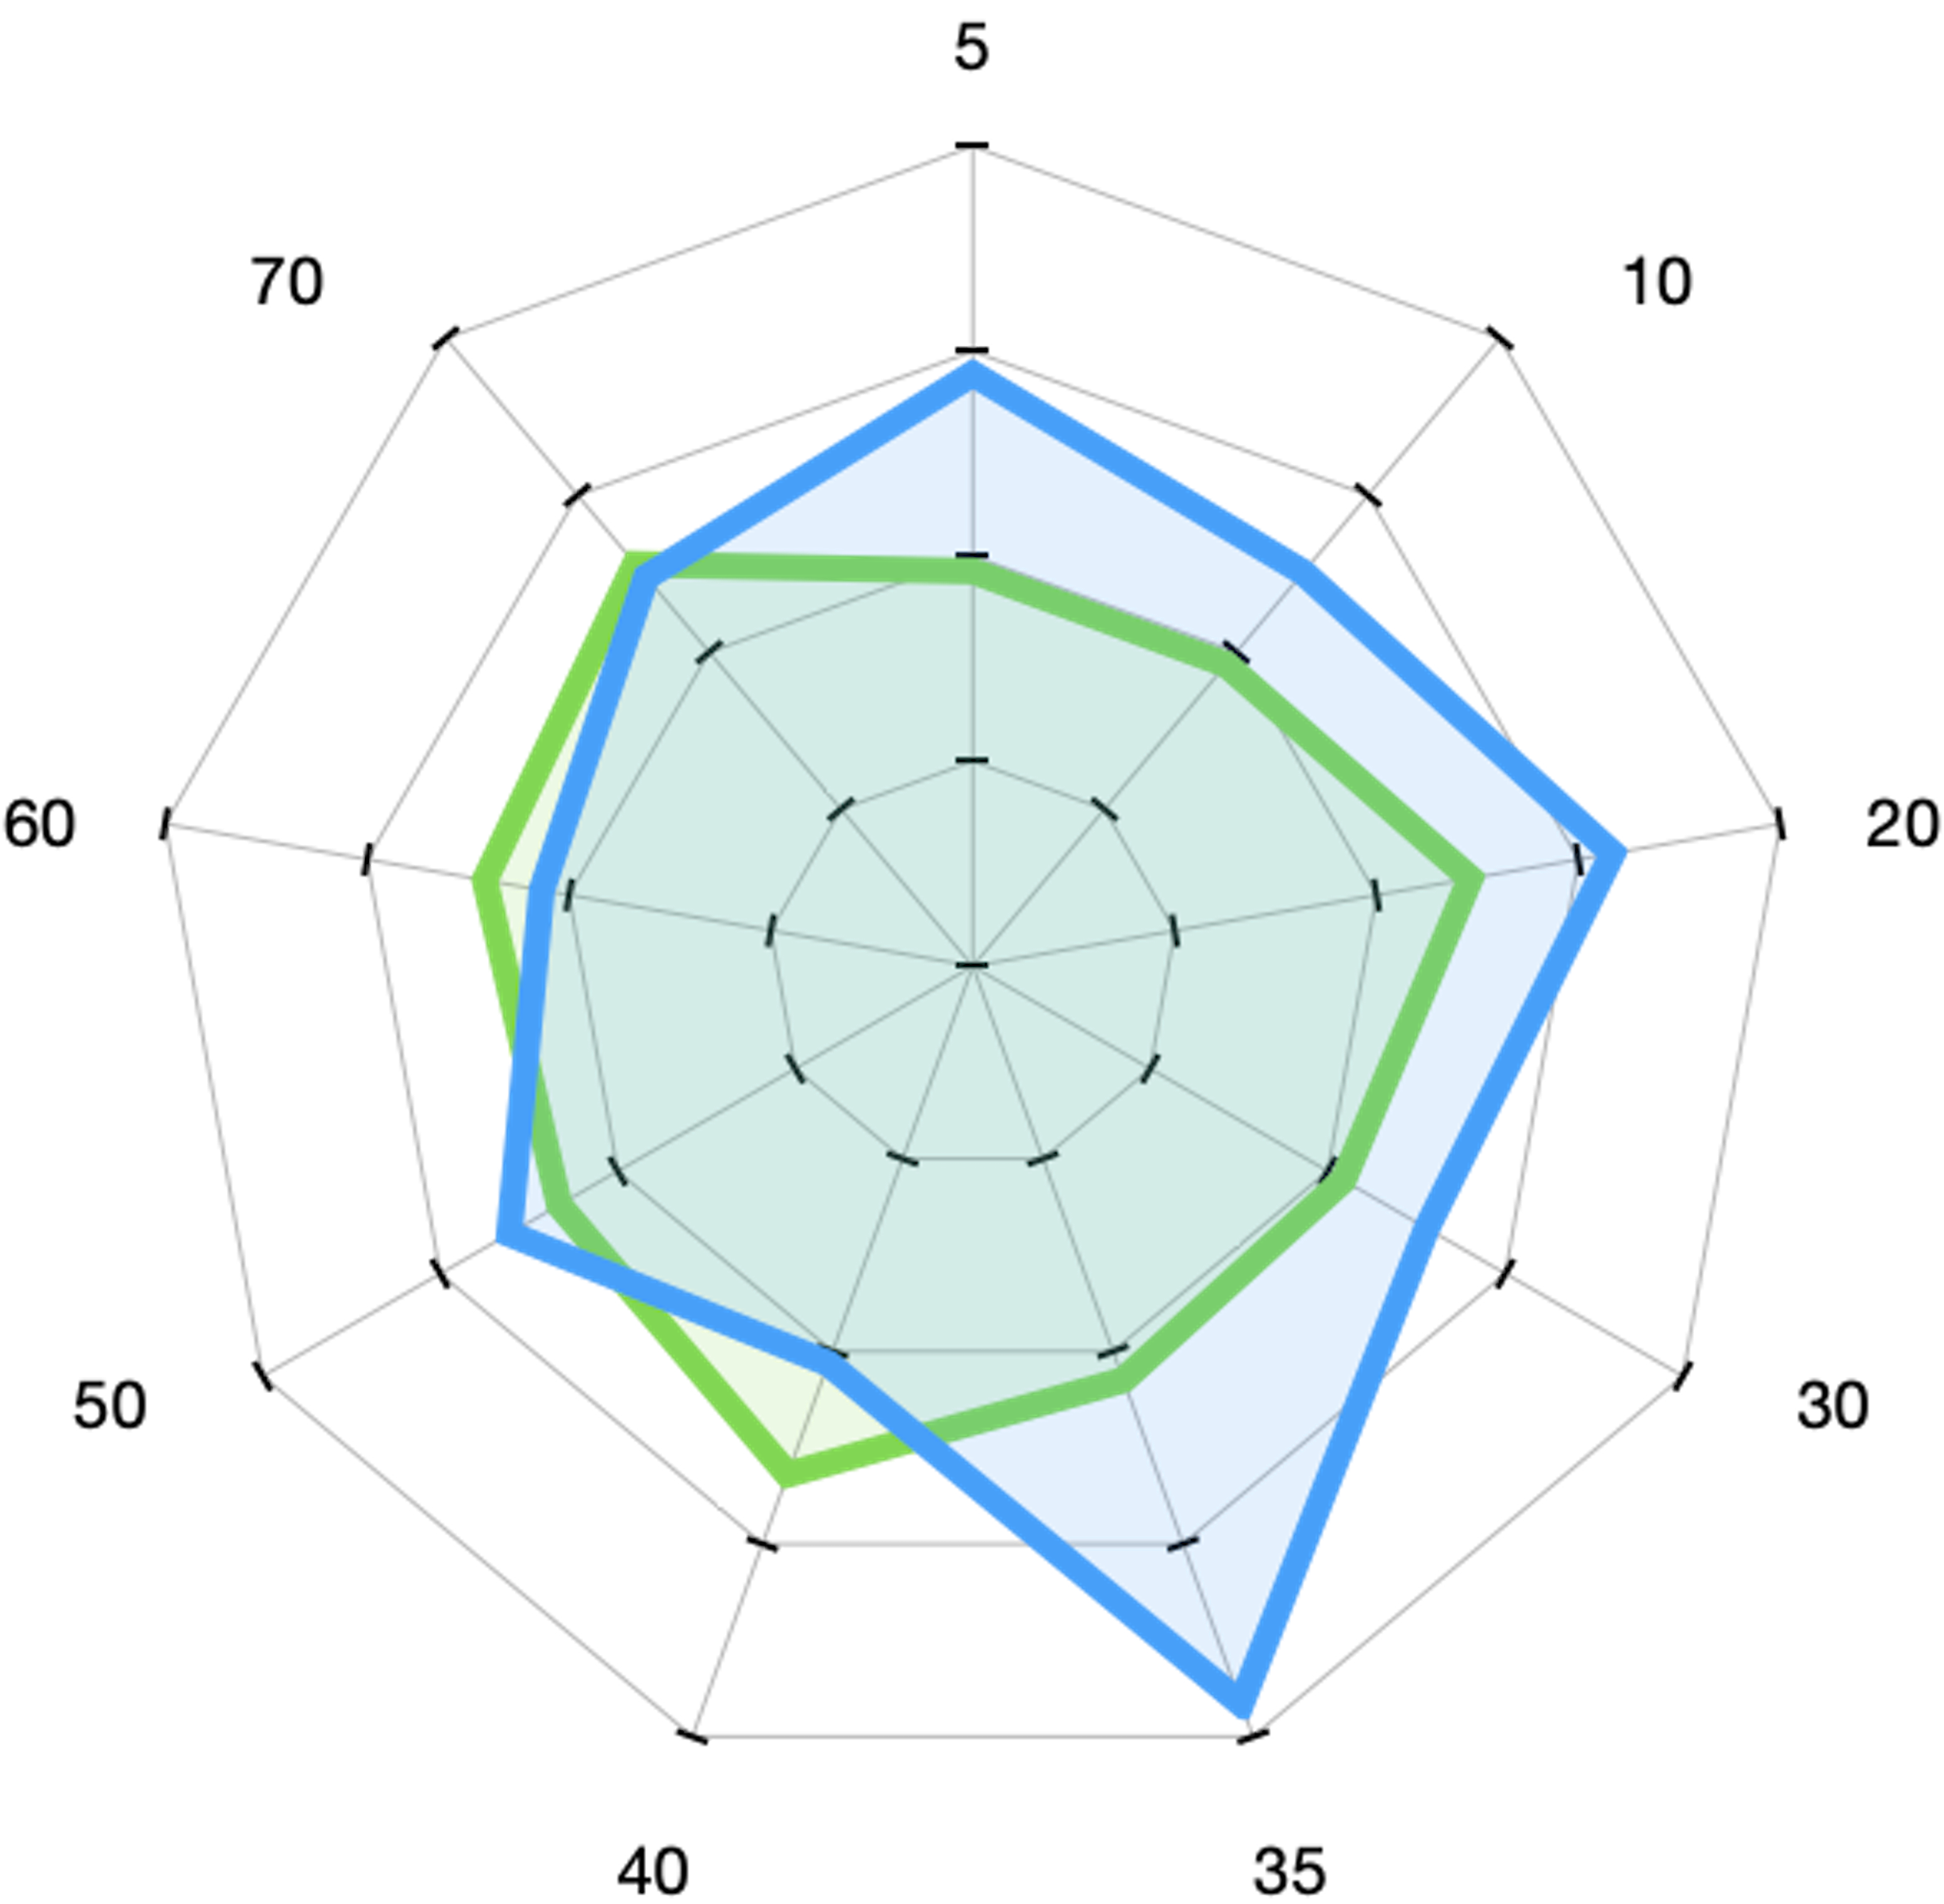
\includegraphics[width=0.4\textwidth, height=0.25\linewidth]{GRU_MAE_SPIDER.png}\label{fig:GRU_MAE_SPIDER}}
  \caption{Comparison of models over MAE}
  \label{fig:all_models_mae}
\end{figure} 
\begin{figure}[ht!]
%\centering
\subfloat[LSTM Vs Proposed LSTM]{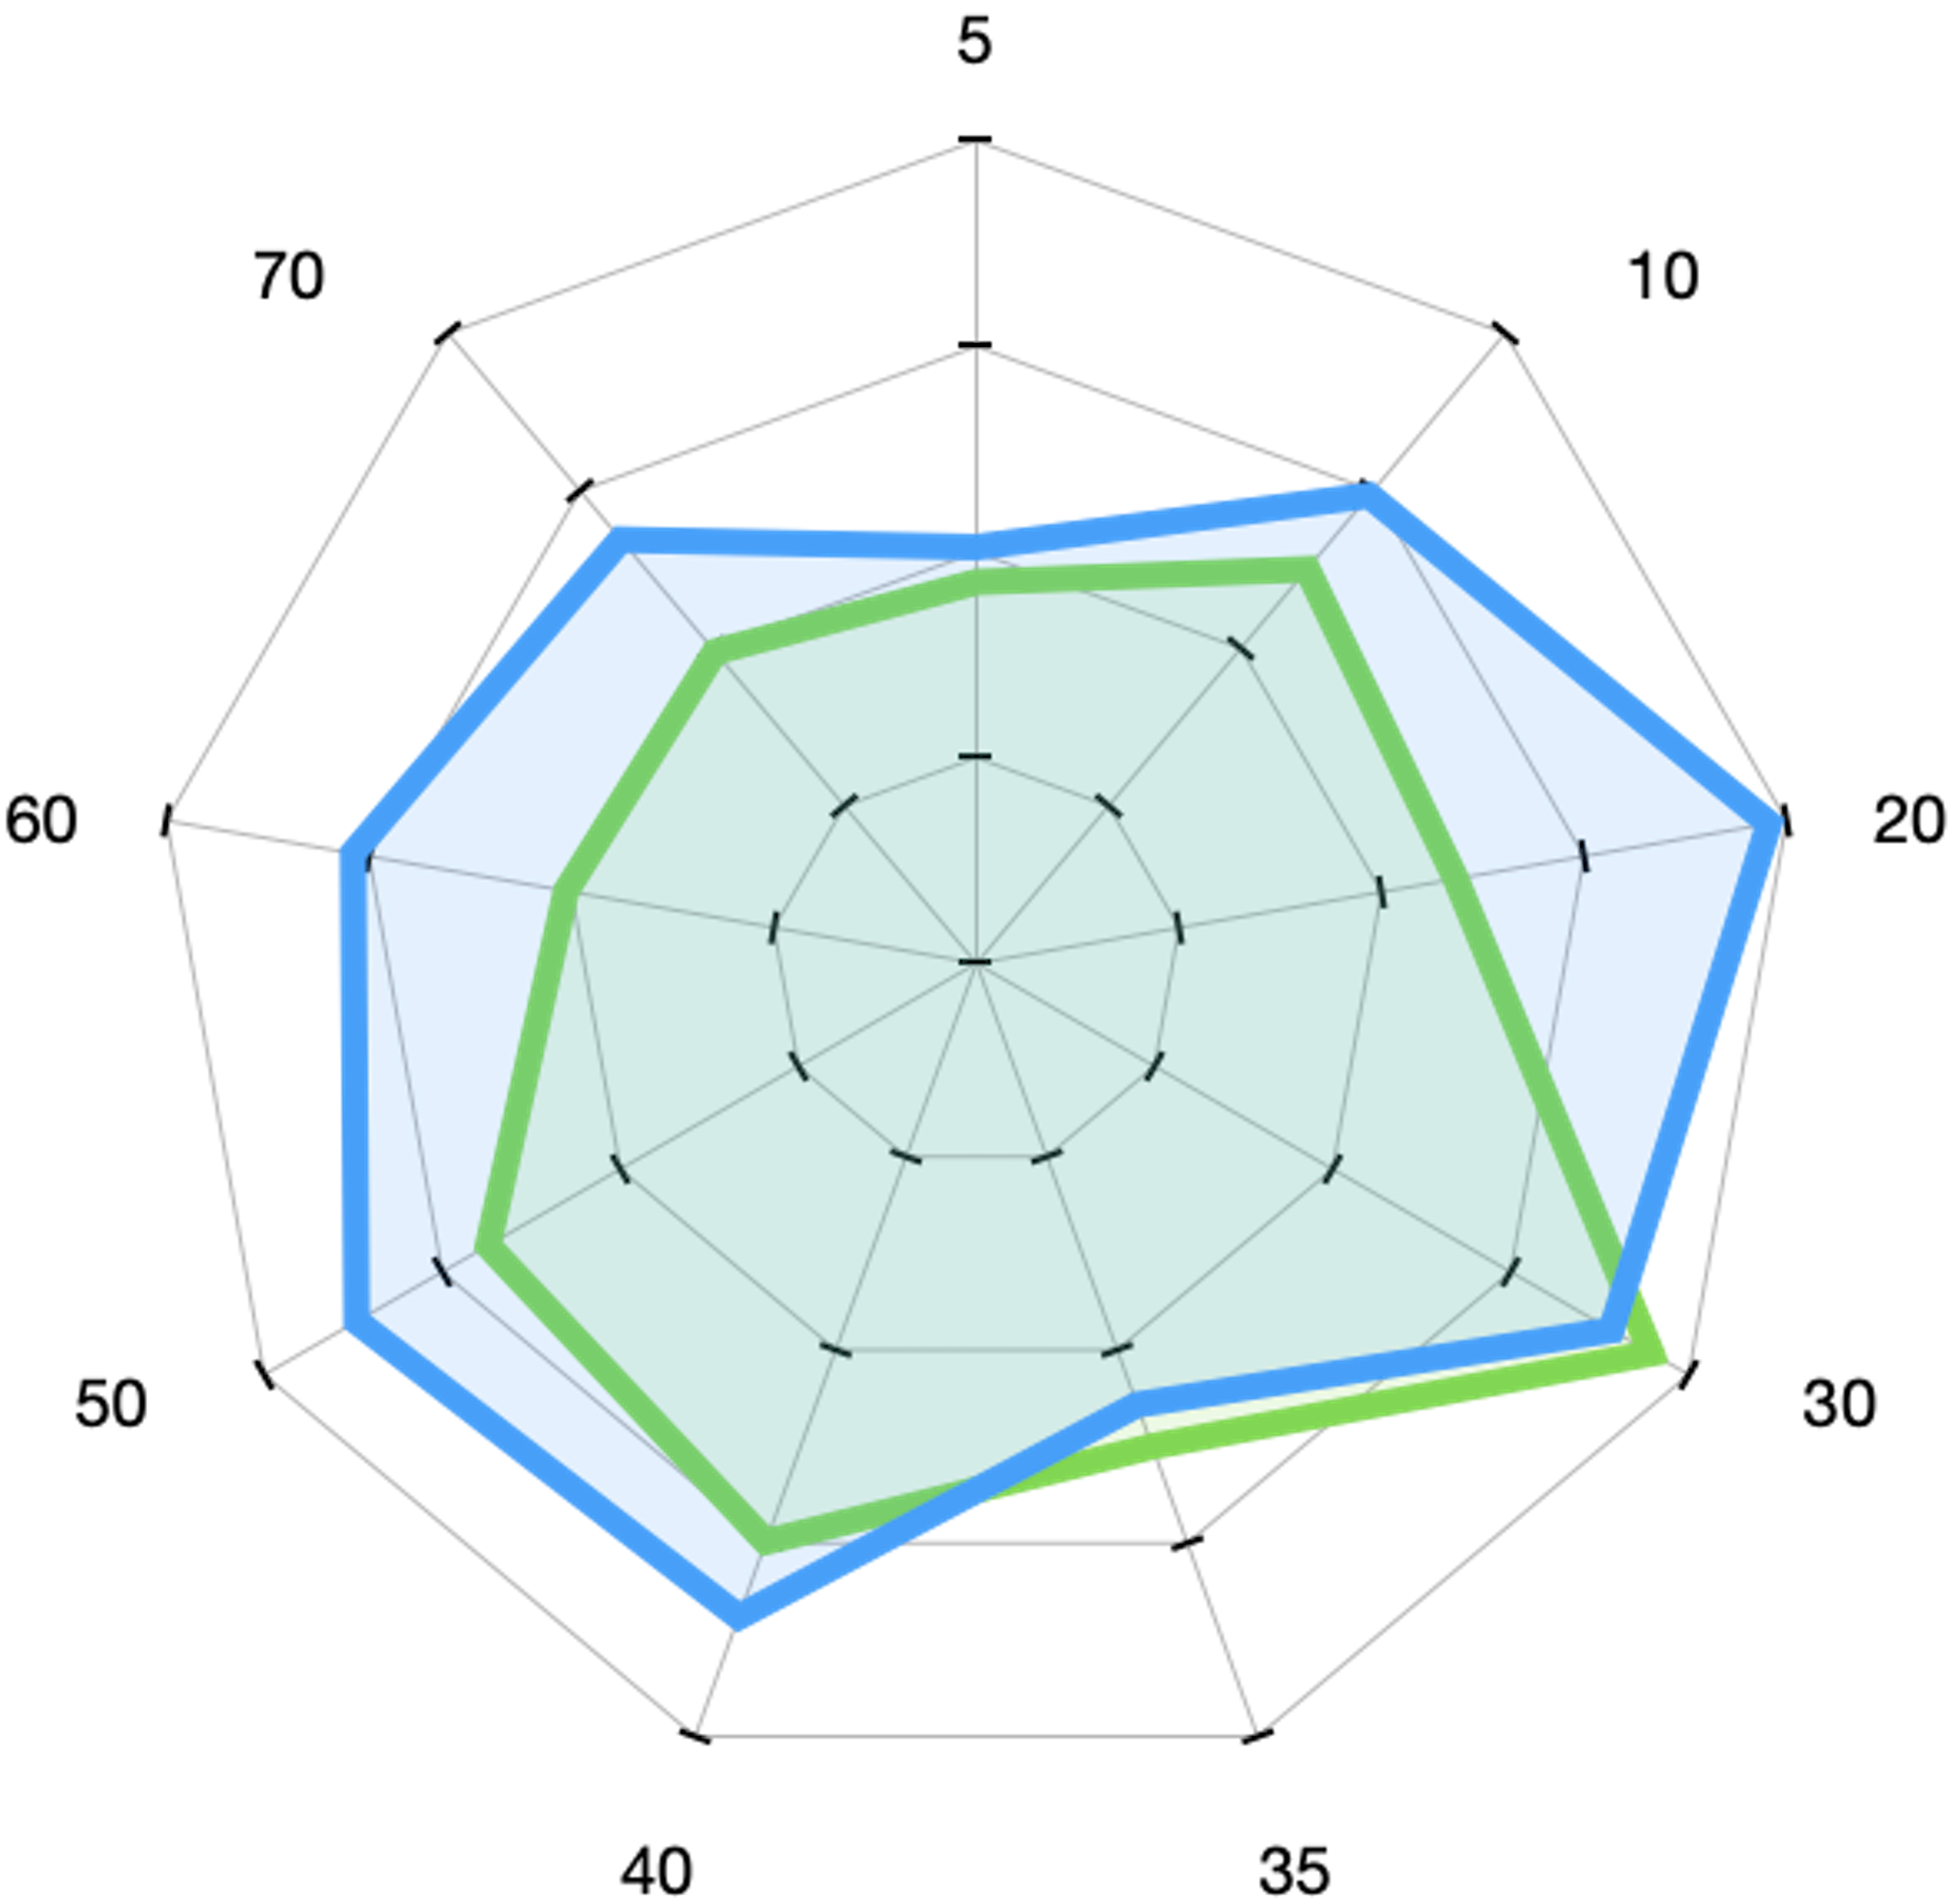
\includegraphics[width=0.4\textwidth, height=0.25\linewidth]{LSTM_MSE_SPIDER.png}\label{fig:LSTM MSE SPIDER}} 
\hfill
\subfloat[RNN Vs Proposed RNN]{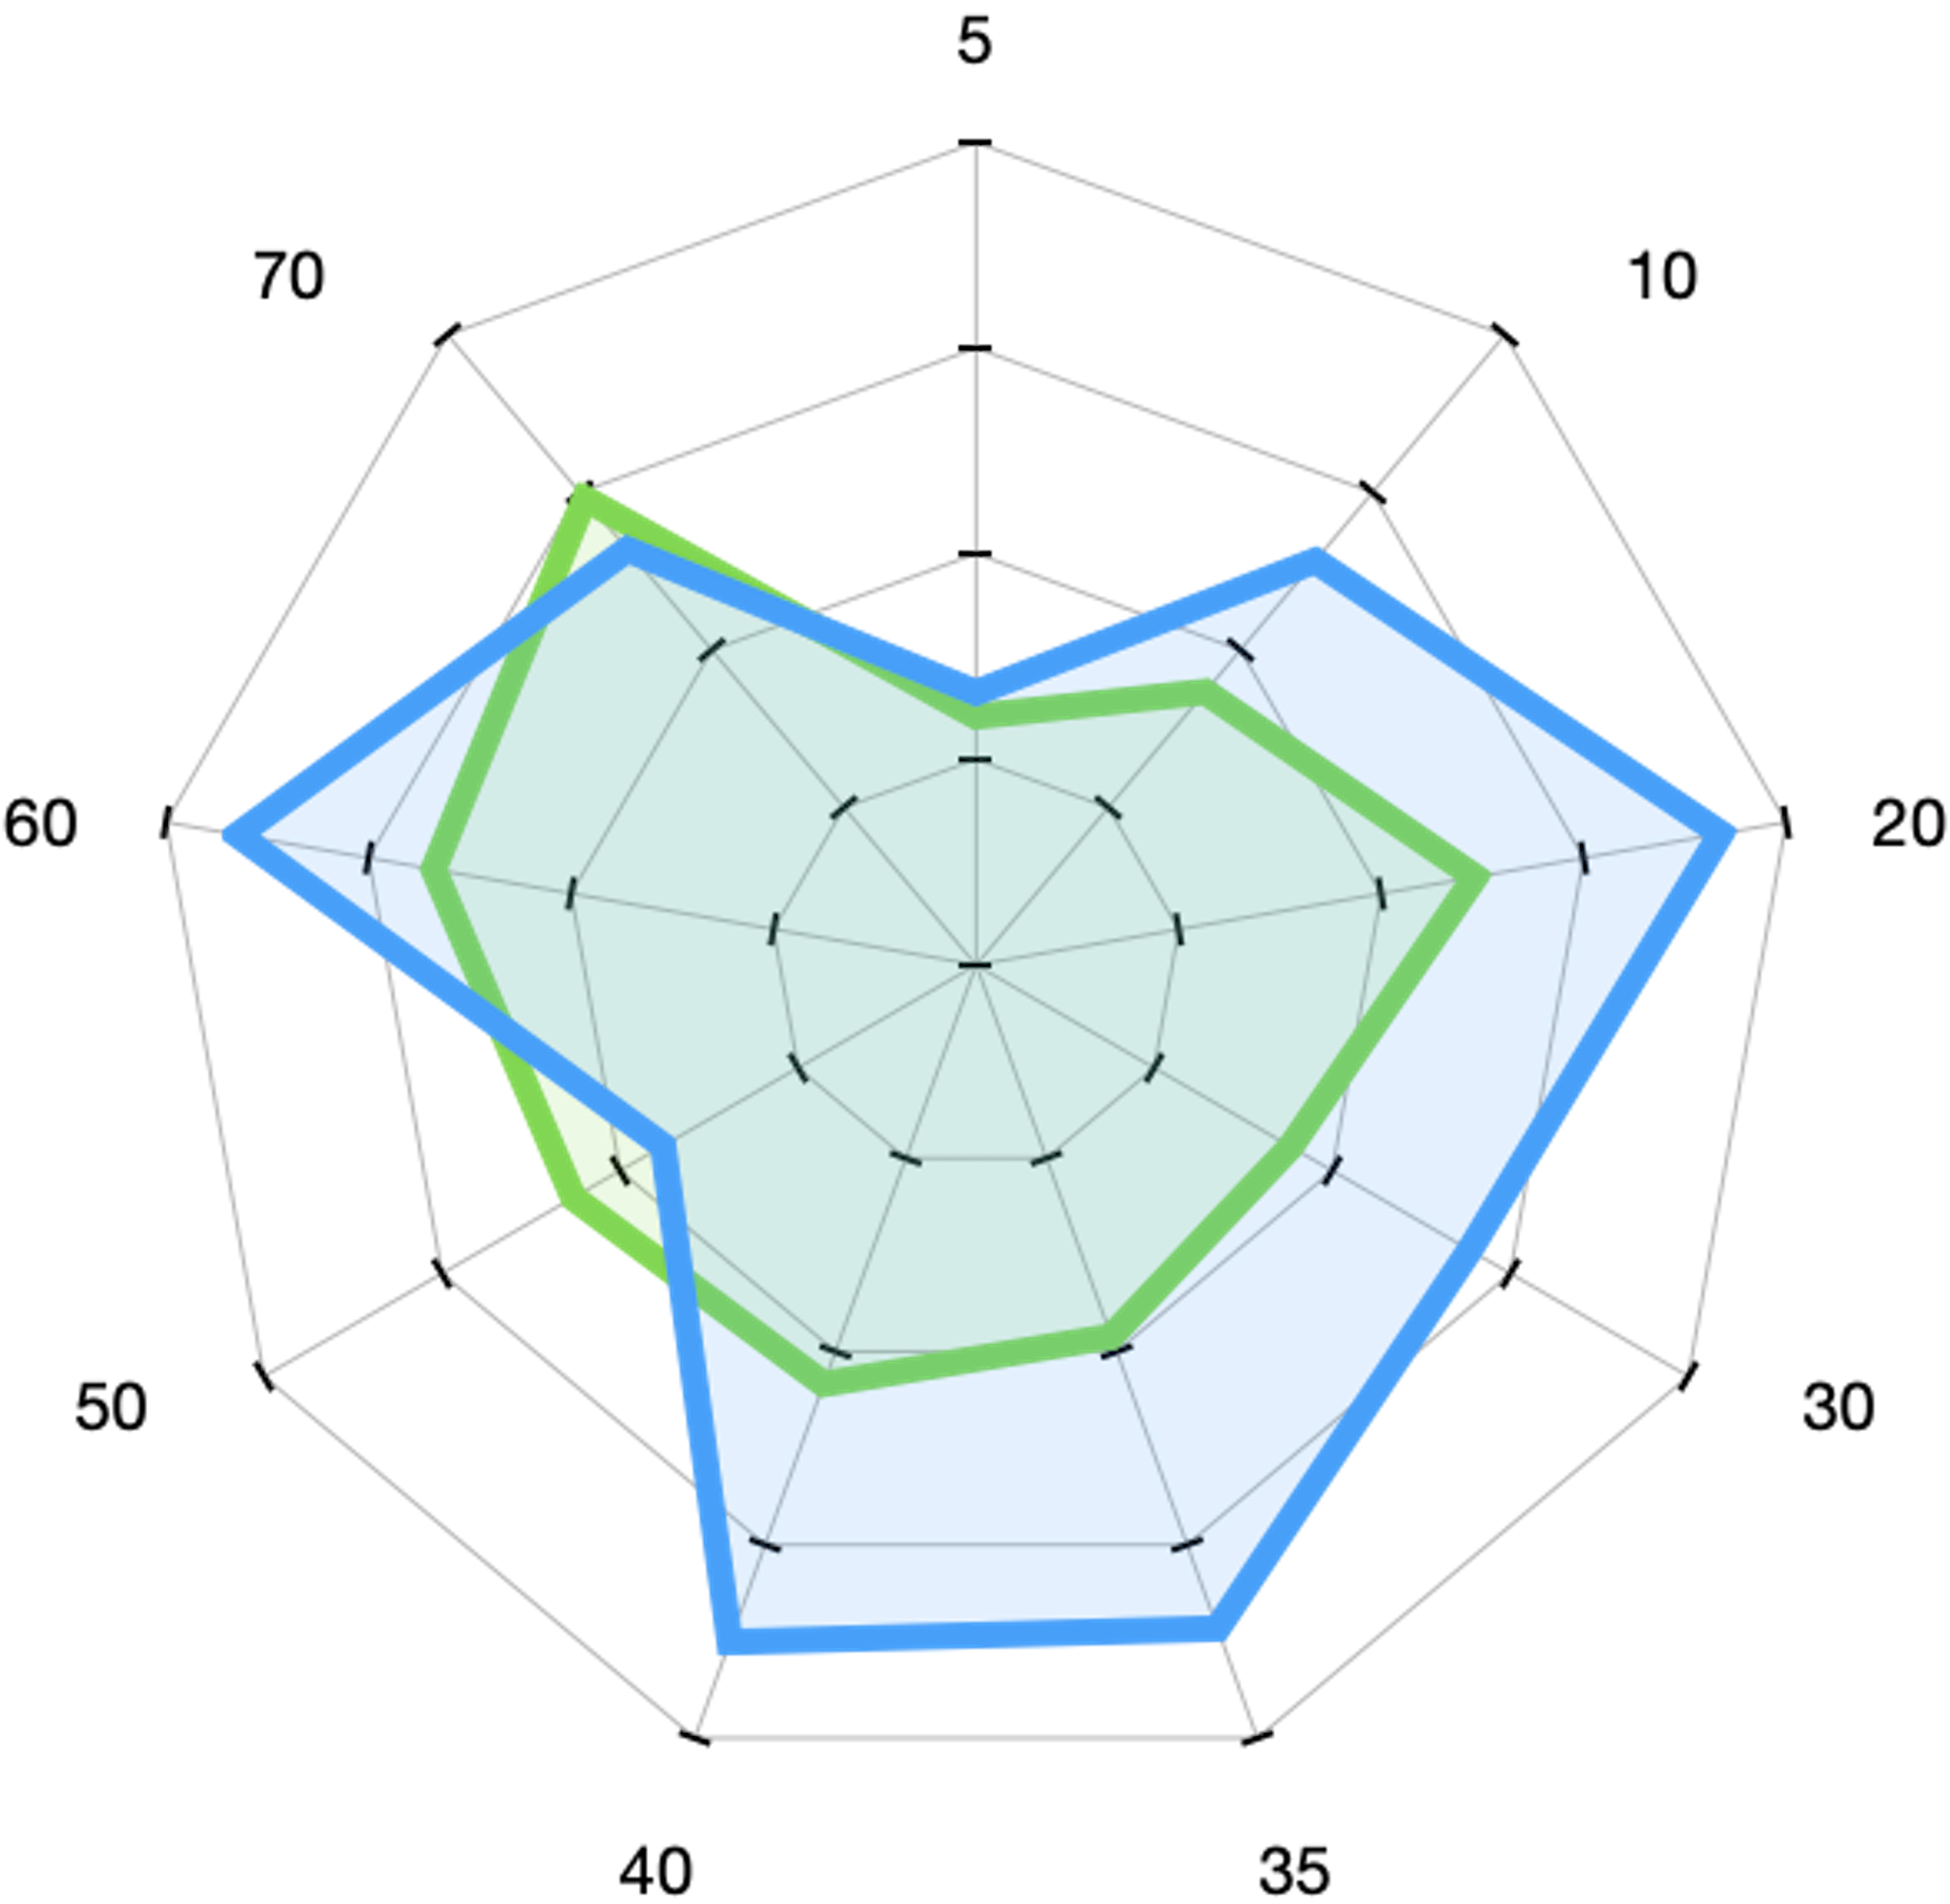
\includegraphics[width=0.4\textwidth, height=0.25\linewidth]{RNN_MSE_SPIDER.png}\label{fig:RNN_MSE_SPIDER}} 
% \vspace{\baselineskip} % Add vertical space between rows
\\
\subfloat[BiLSTM Vs Proposed RNN]{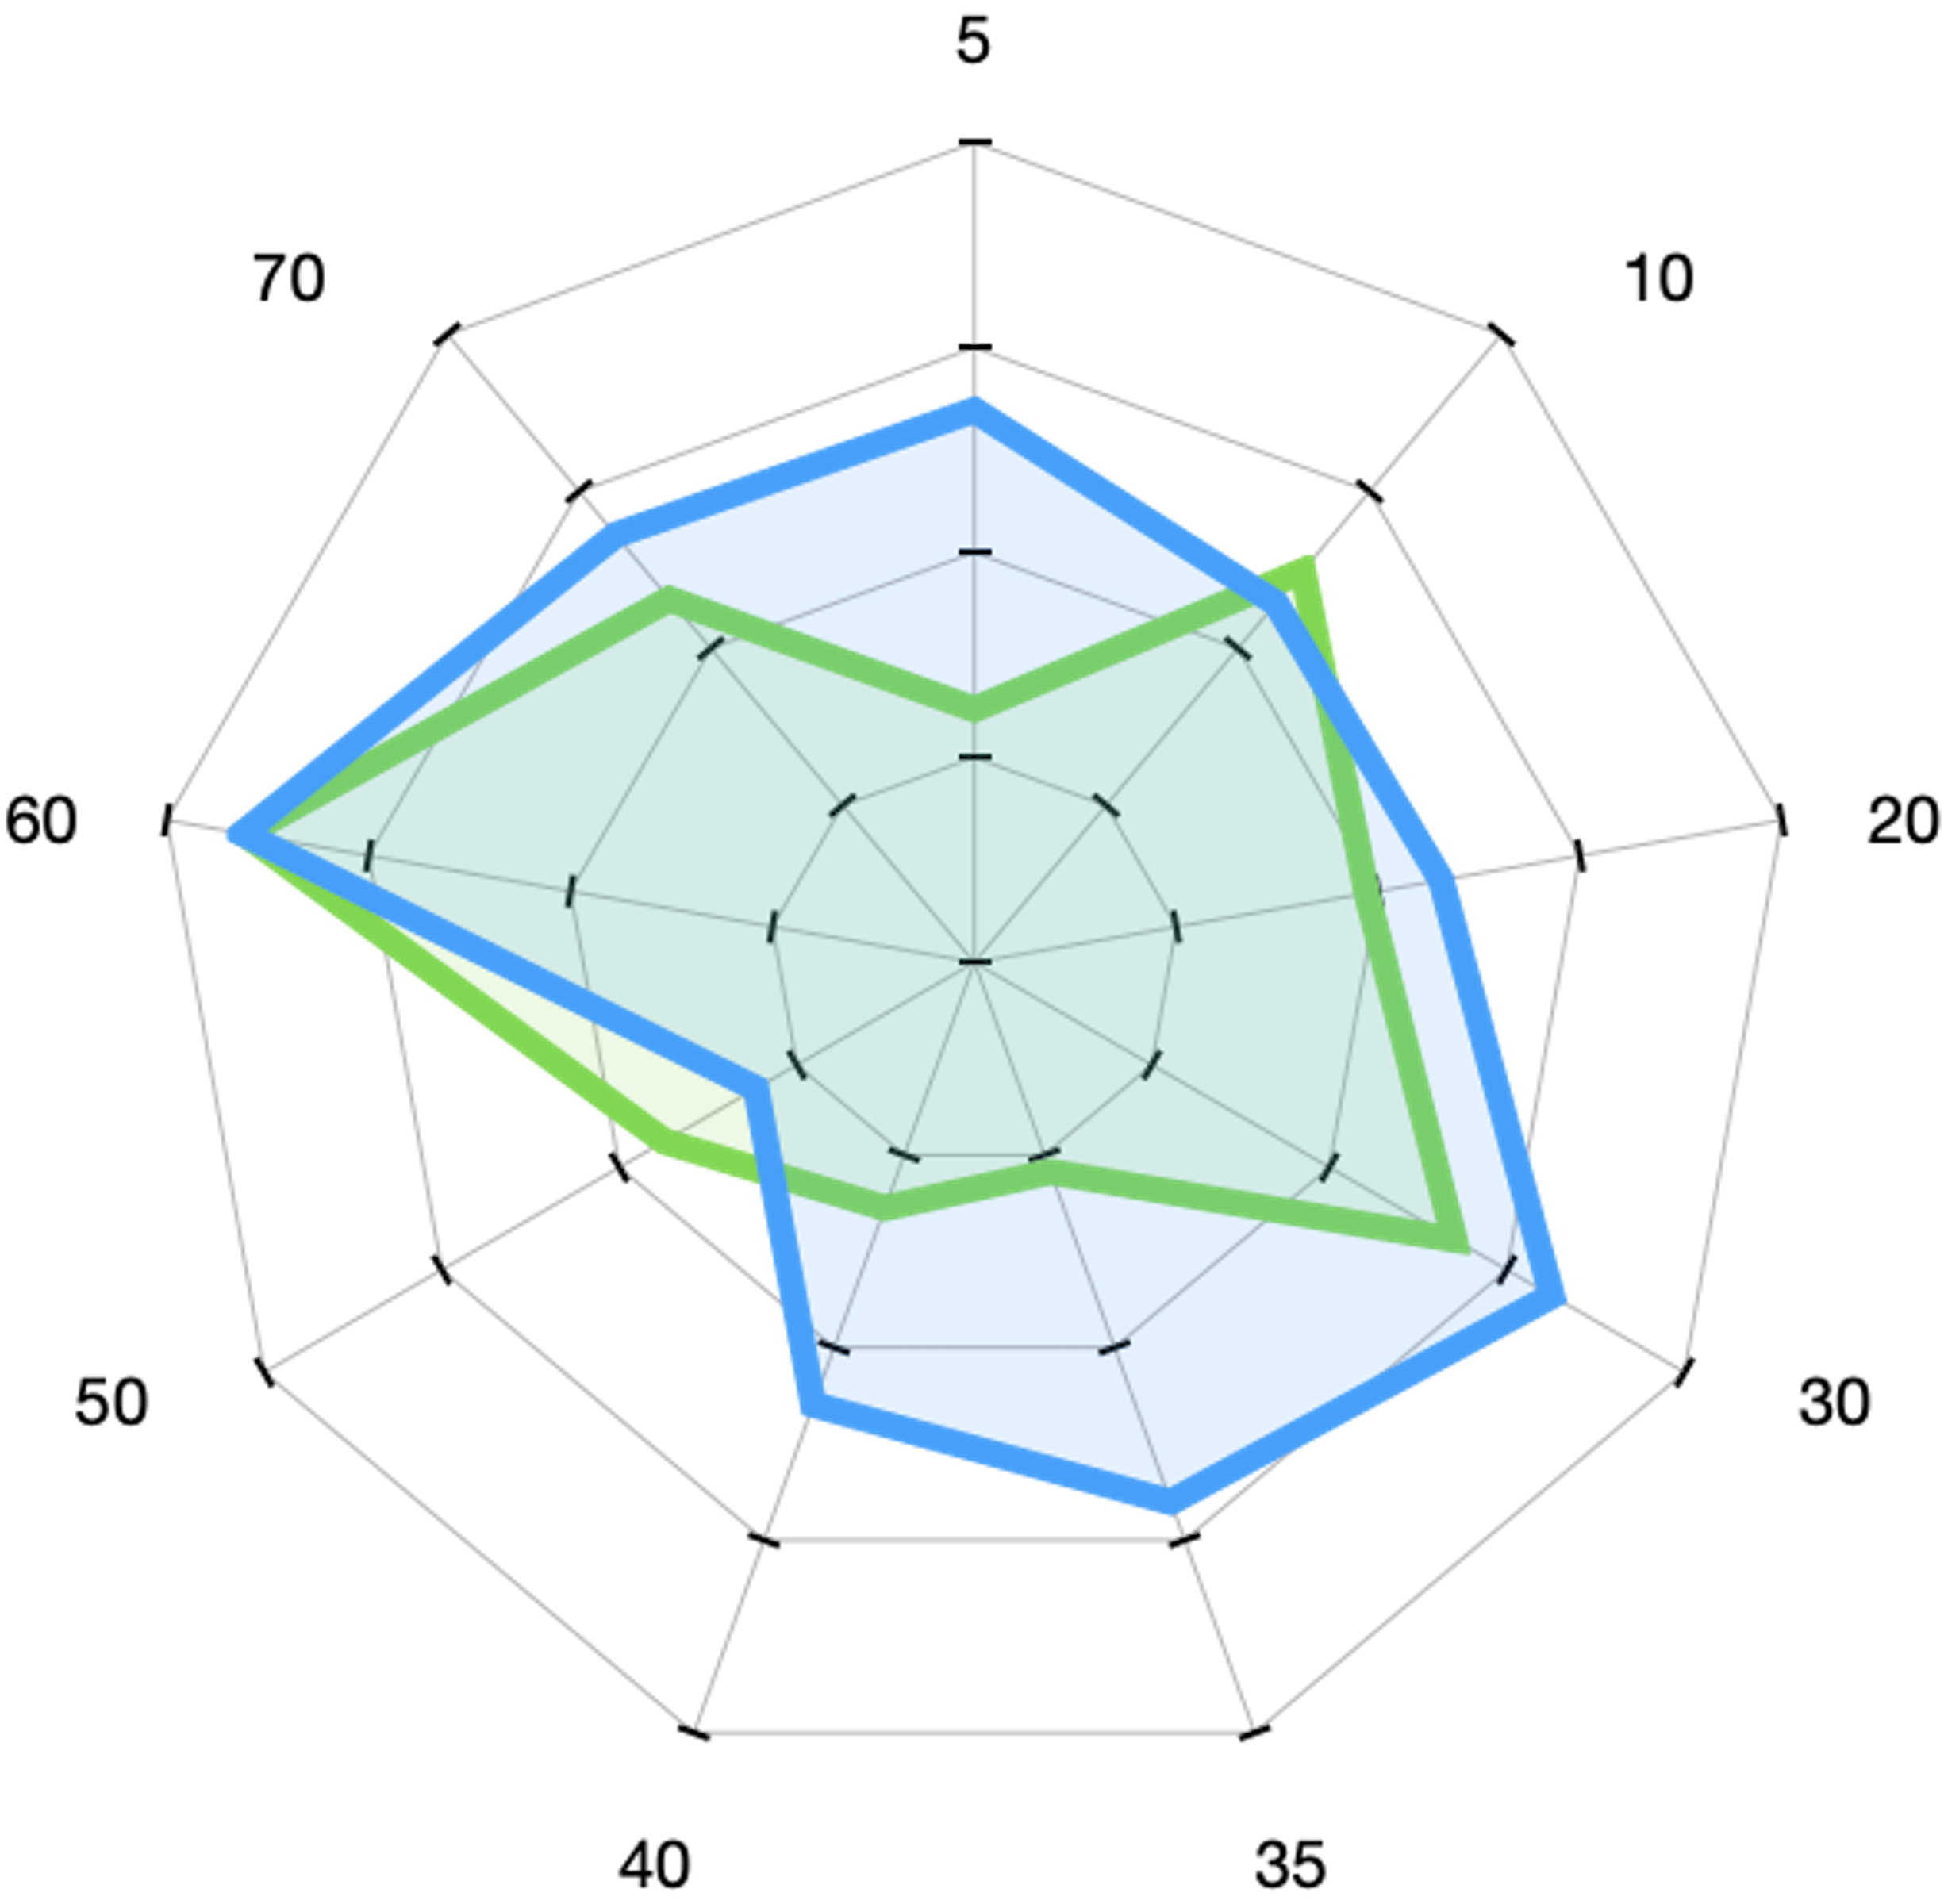
\includegraphics[width=0.4\textwidth, height=0.25\linewidth]{BI-LSTM_MSE_SPIDER.png}\label{fig:BiLSTM_MSE_SPIDER}}
\hfill
\subfloat[GRU Vs Proposed GRU]{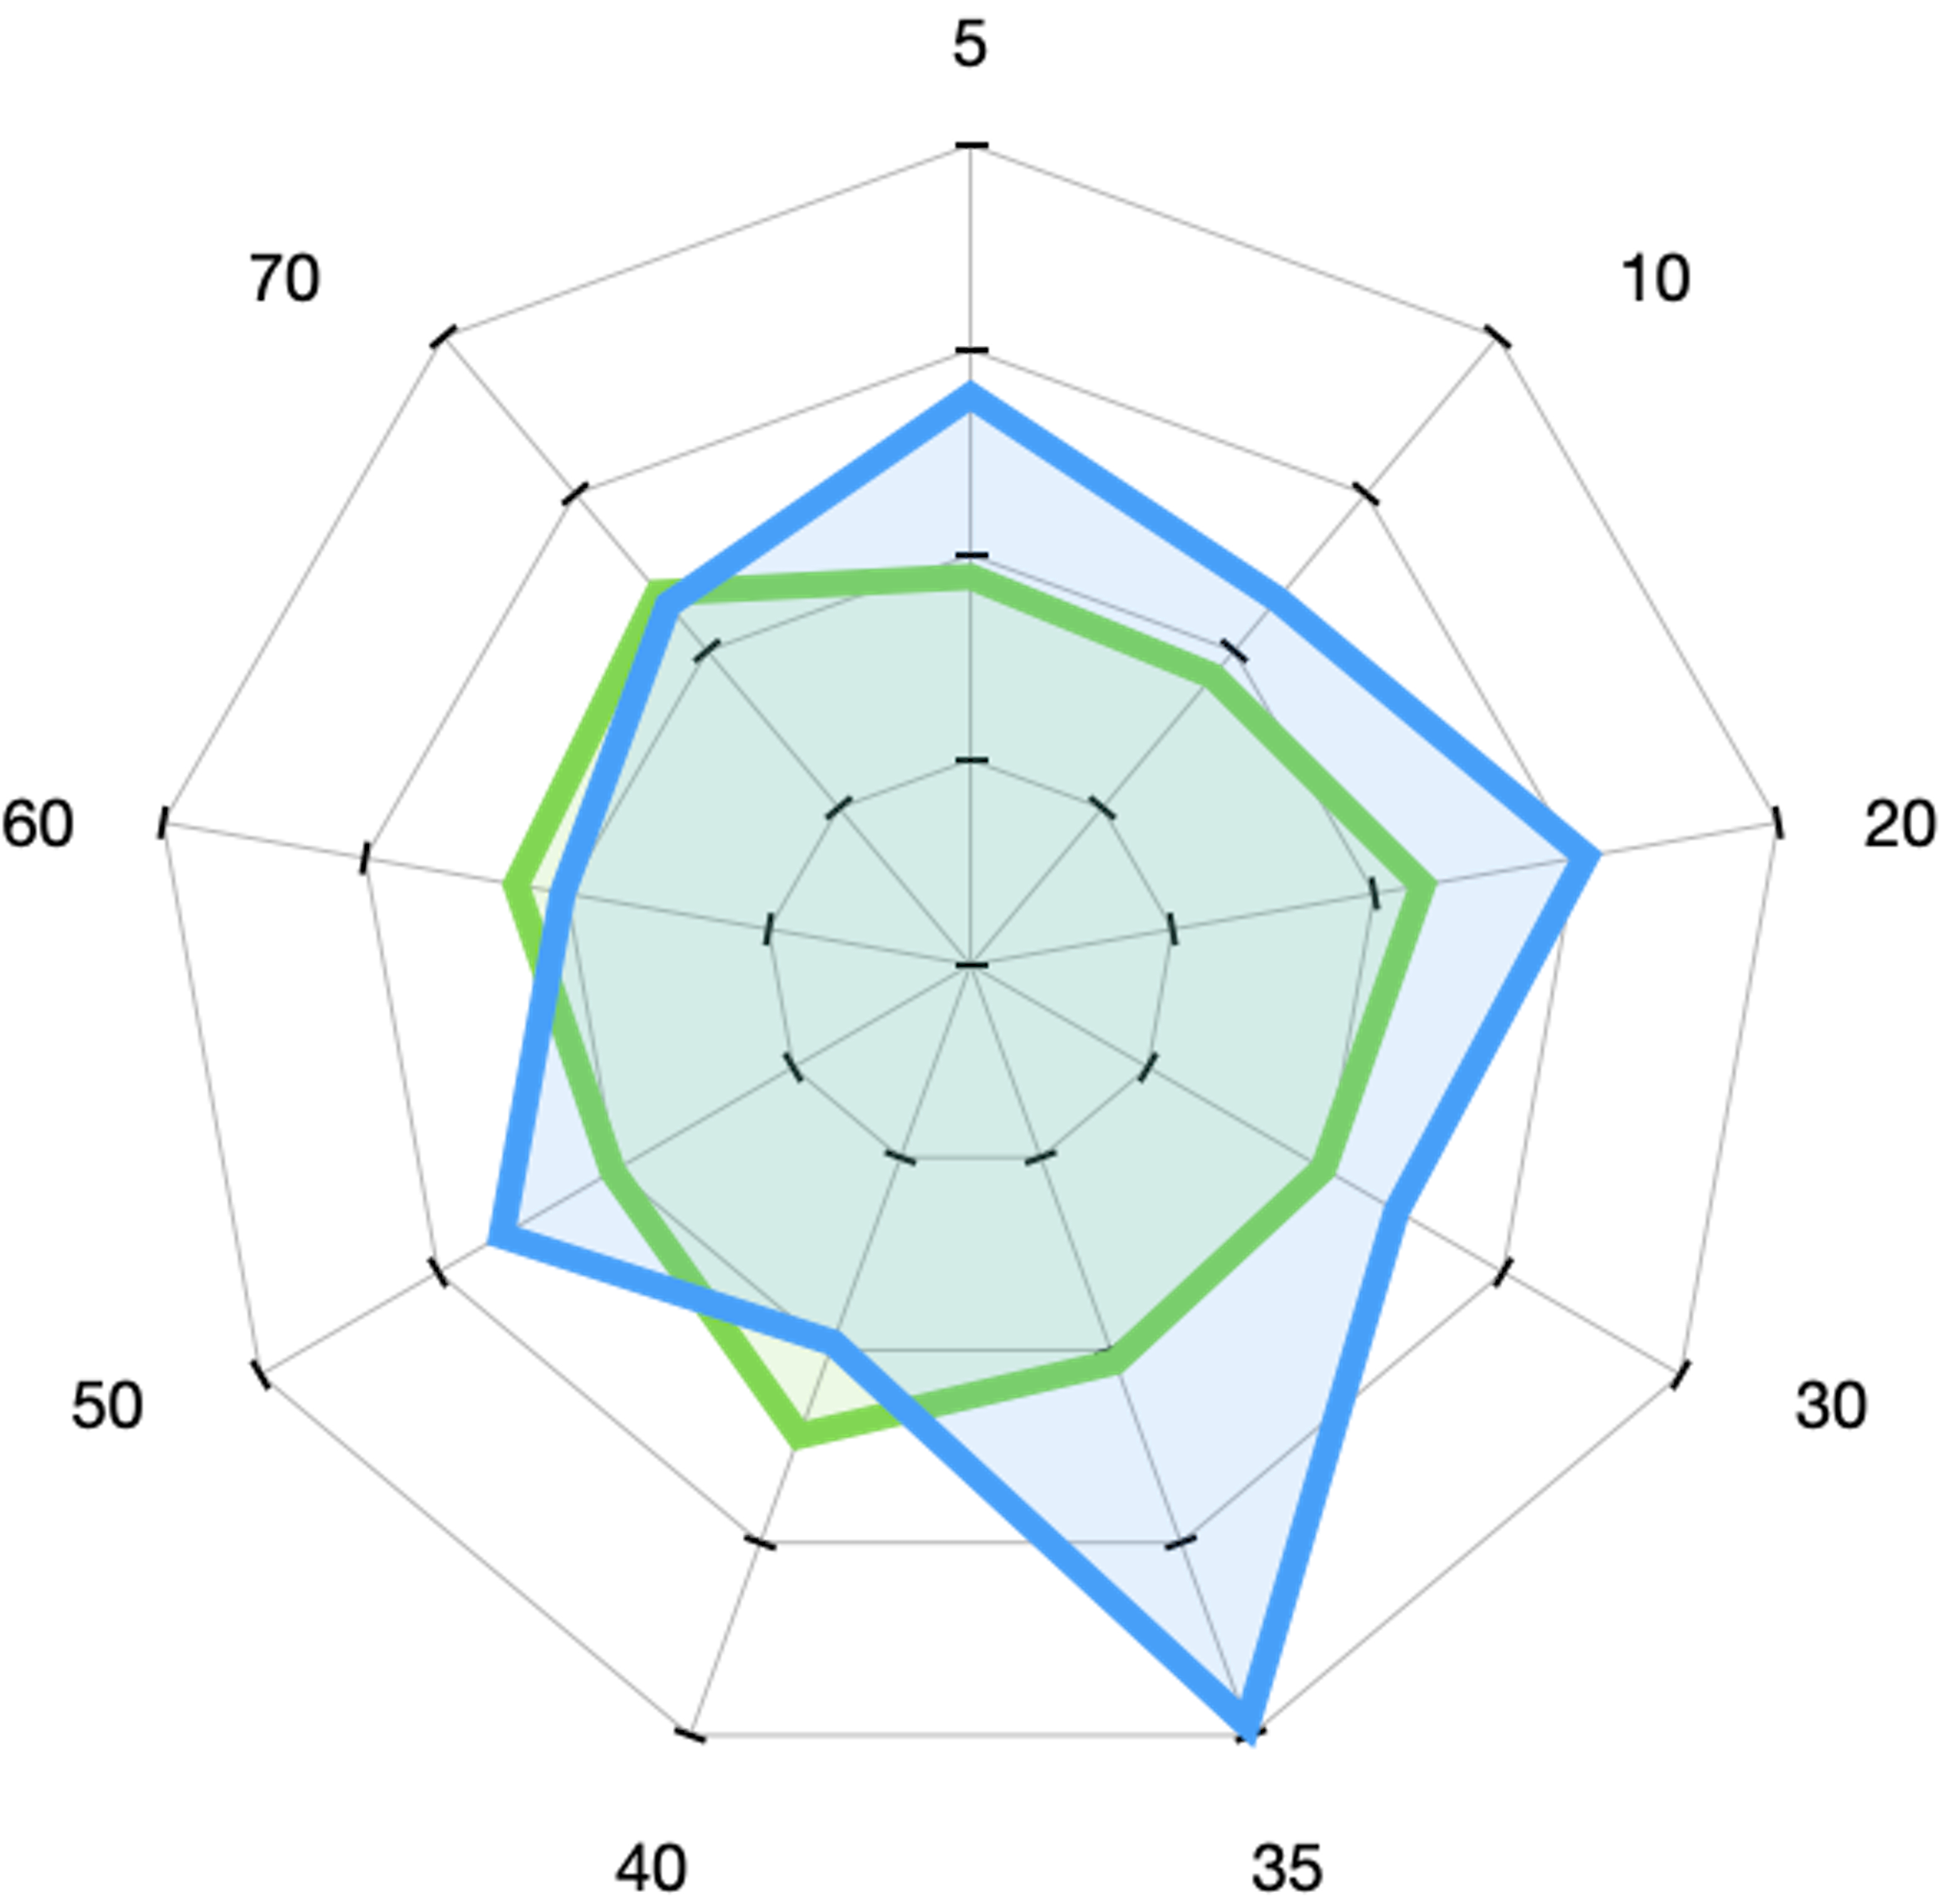
\includegraphics[width=0.4\textwidth, height=0.25\linewidth]{GRU_MSE_SPIDER.png}\label{fig:GRU_MSE_SPIDER}} 
  \caption{Comparison of models over MSE}
  \label{fig:all_models_mse}
\end{figure} 


\begin{figure}[ht!]
%\centering
\subfloat[LSTM Vs Proposed LSTM]{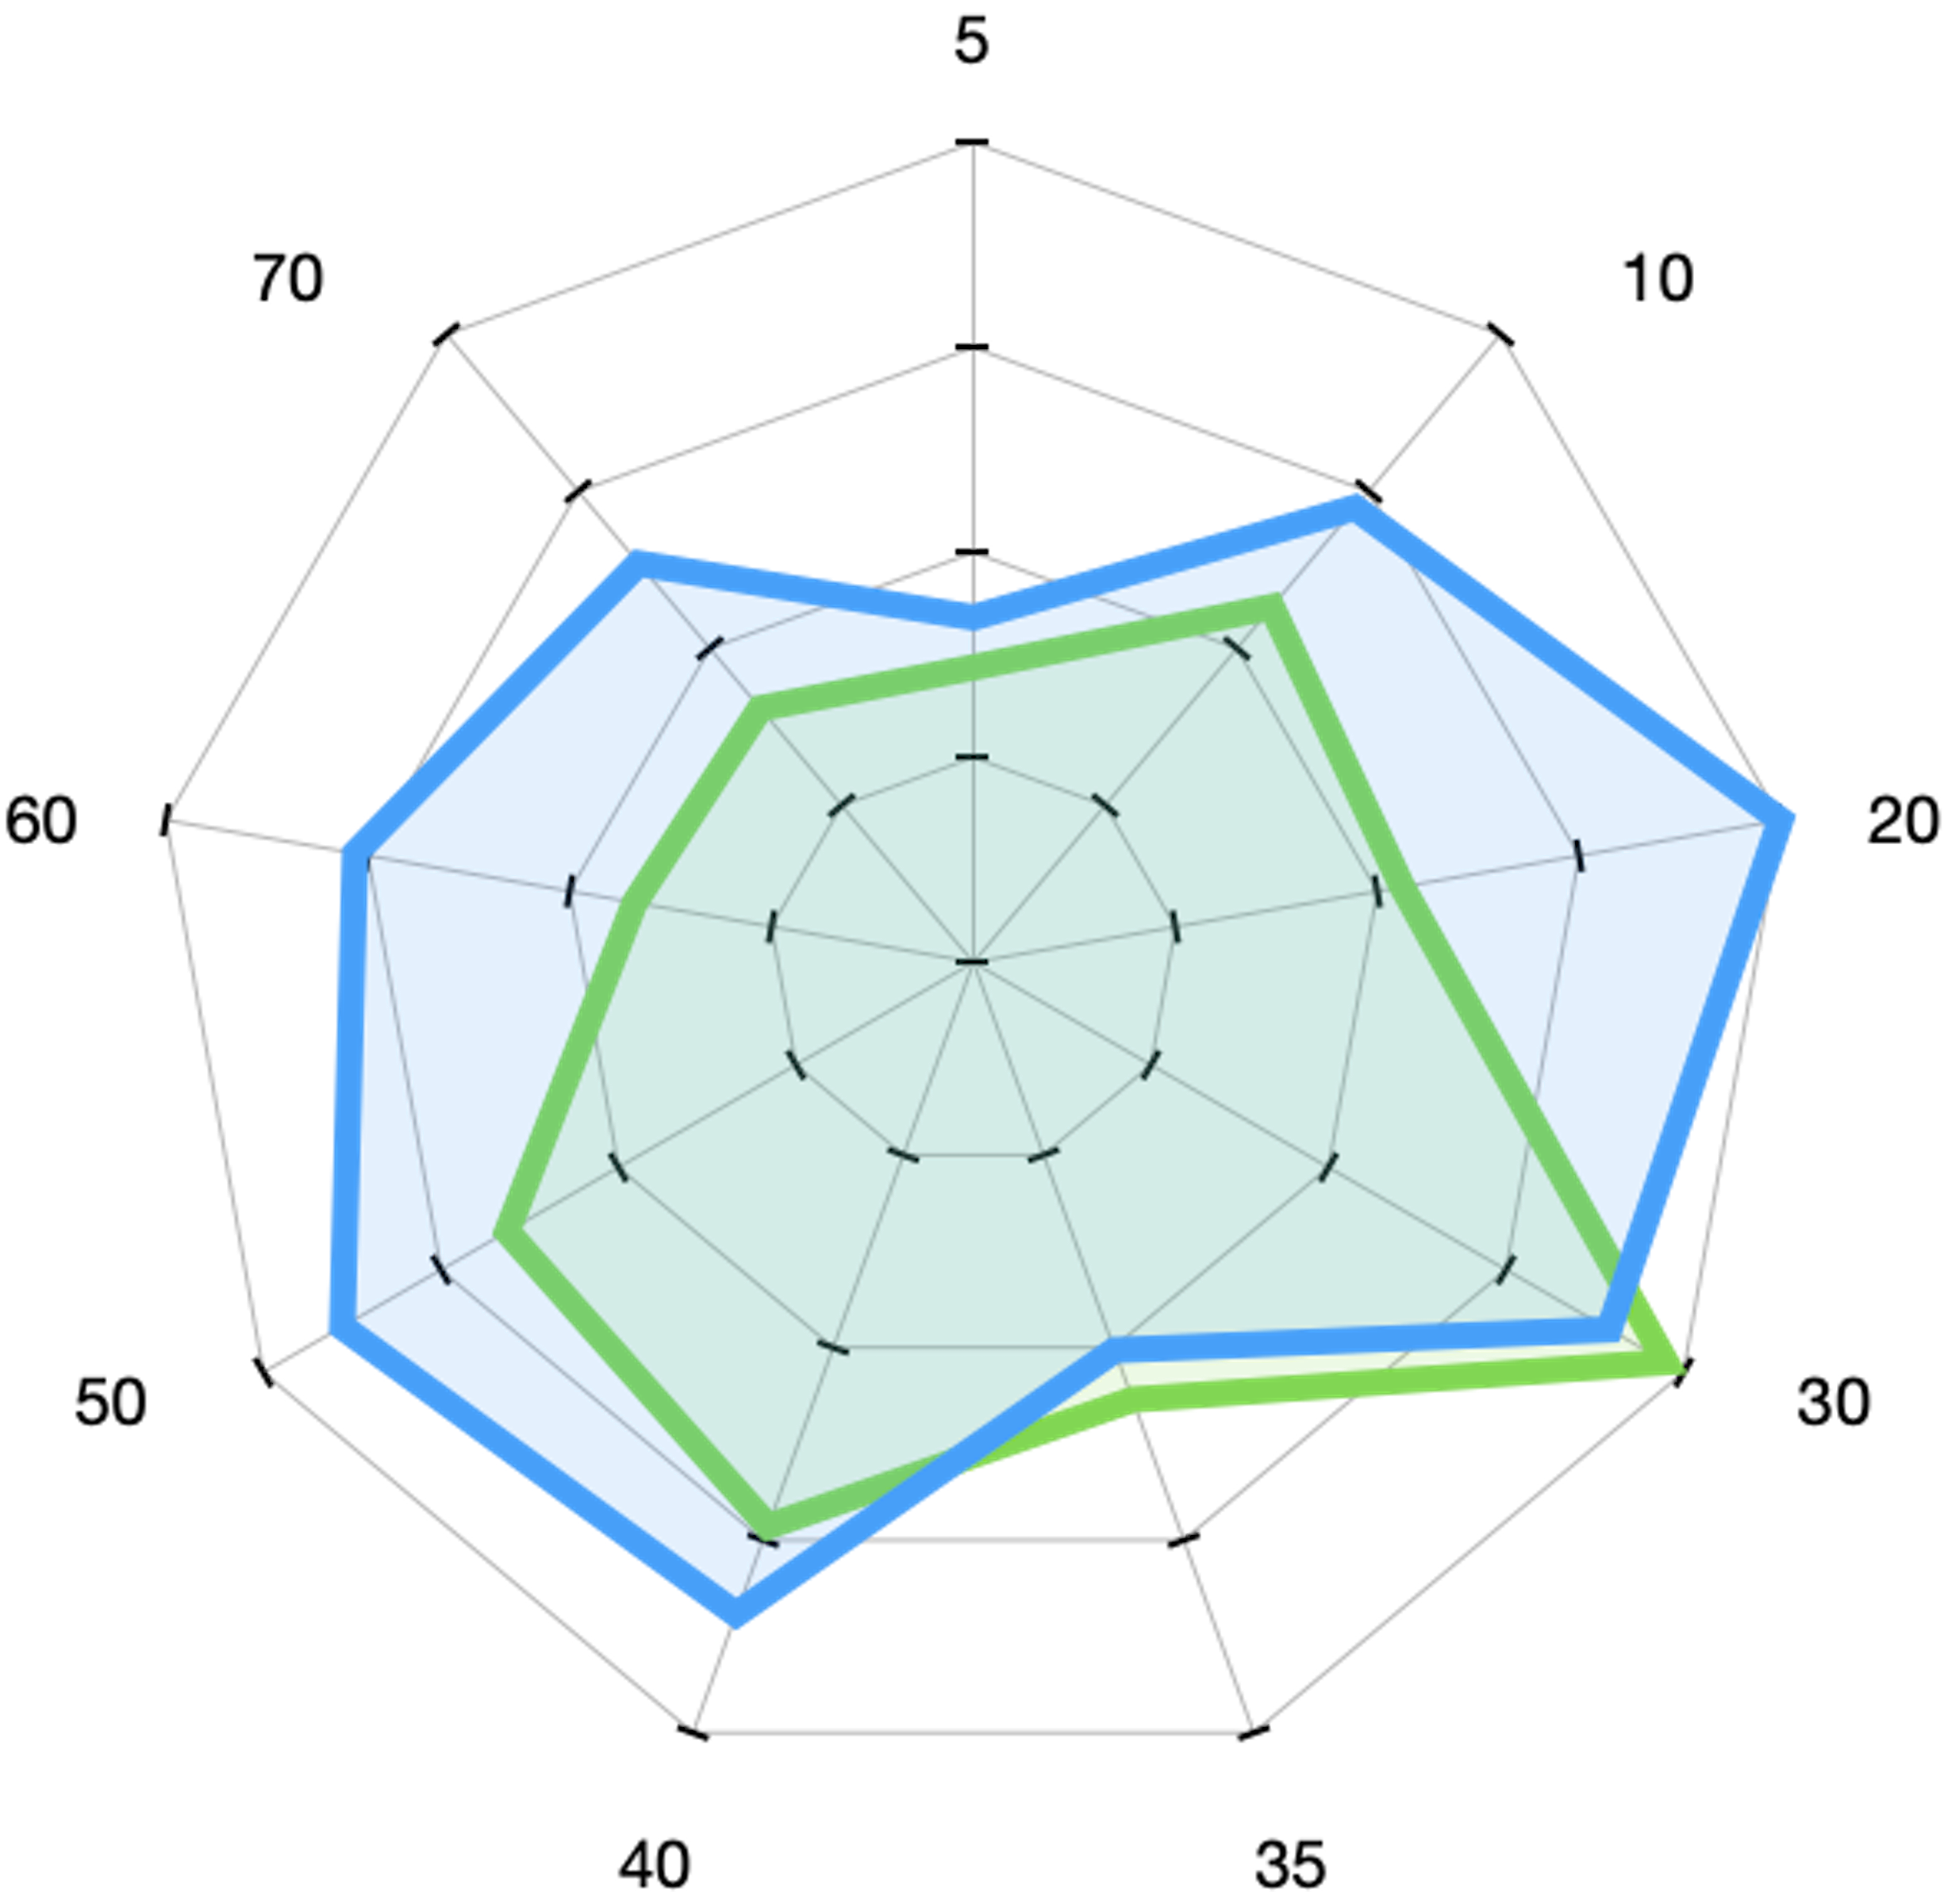
\includegraphics[width=0.4\textwidth, height=0.25\linewidth]{LSTM_RMSE_SPIDER.png}\label{fig:LSTM RMSE SPIDER}}
\hfill
\subfloat[RNN Vs Proposed RNN]{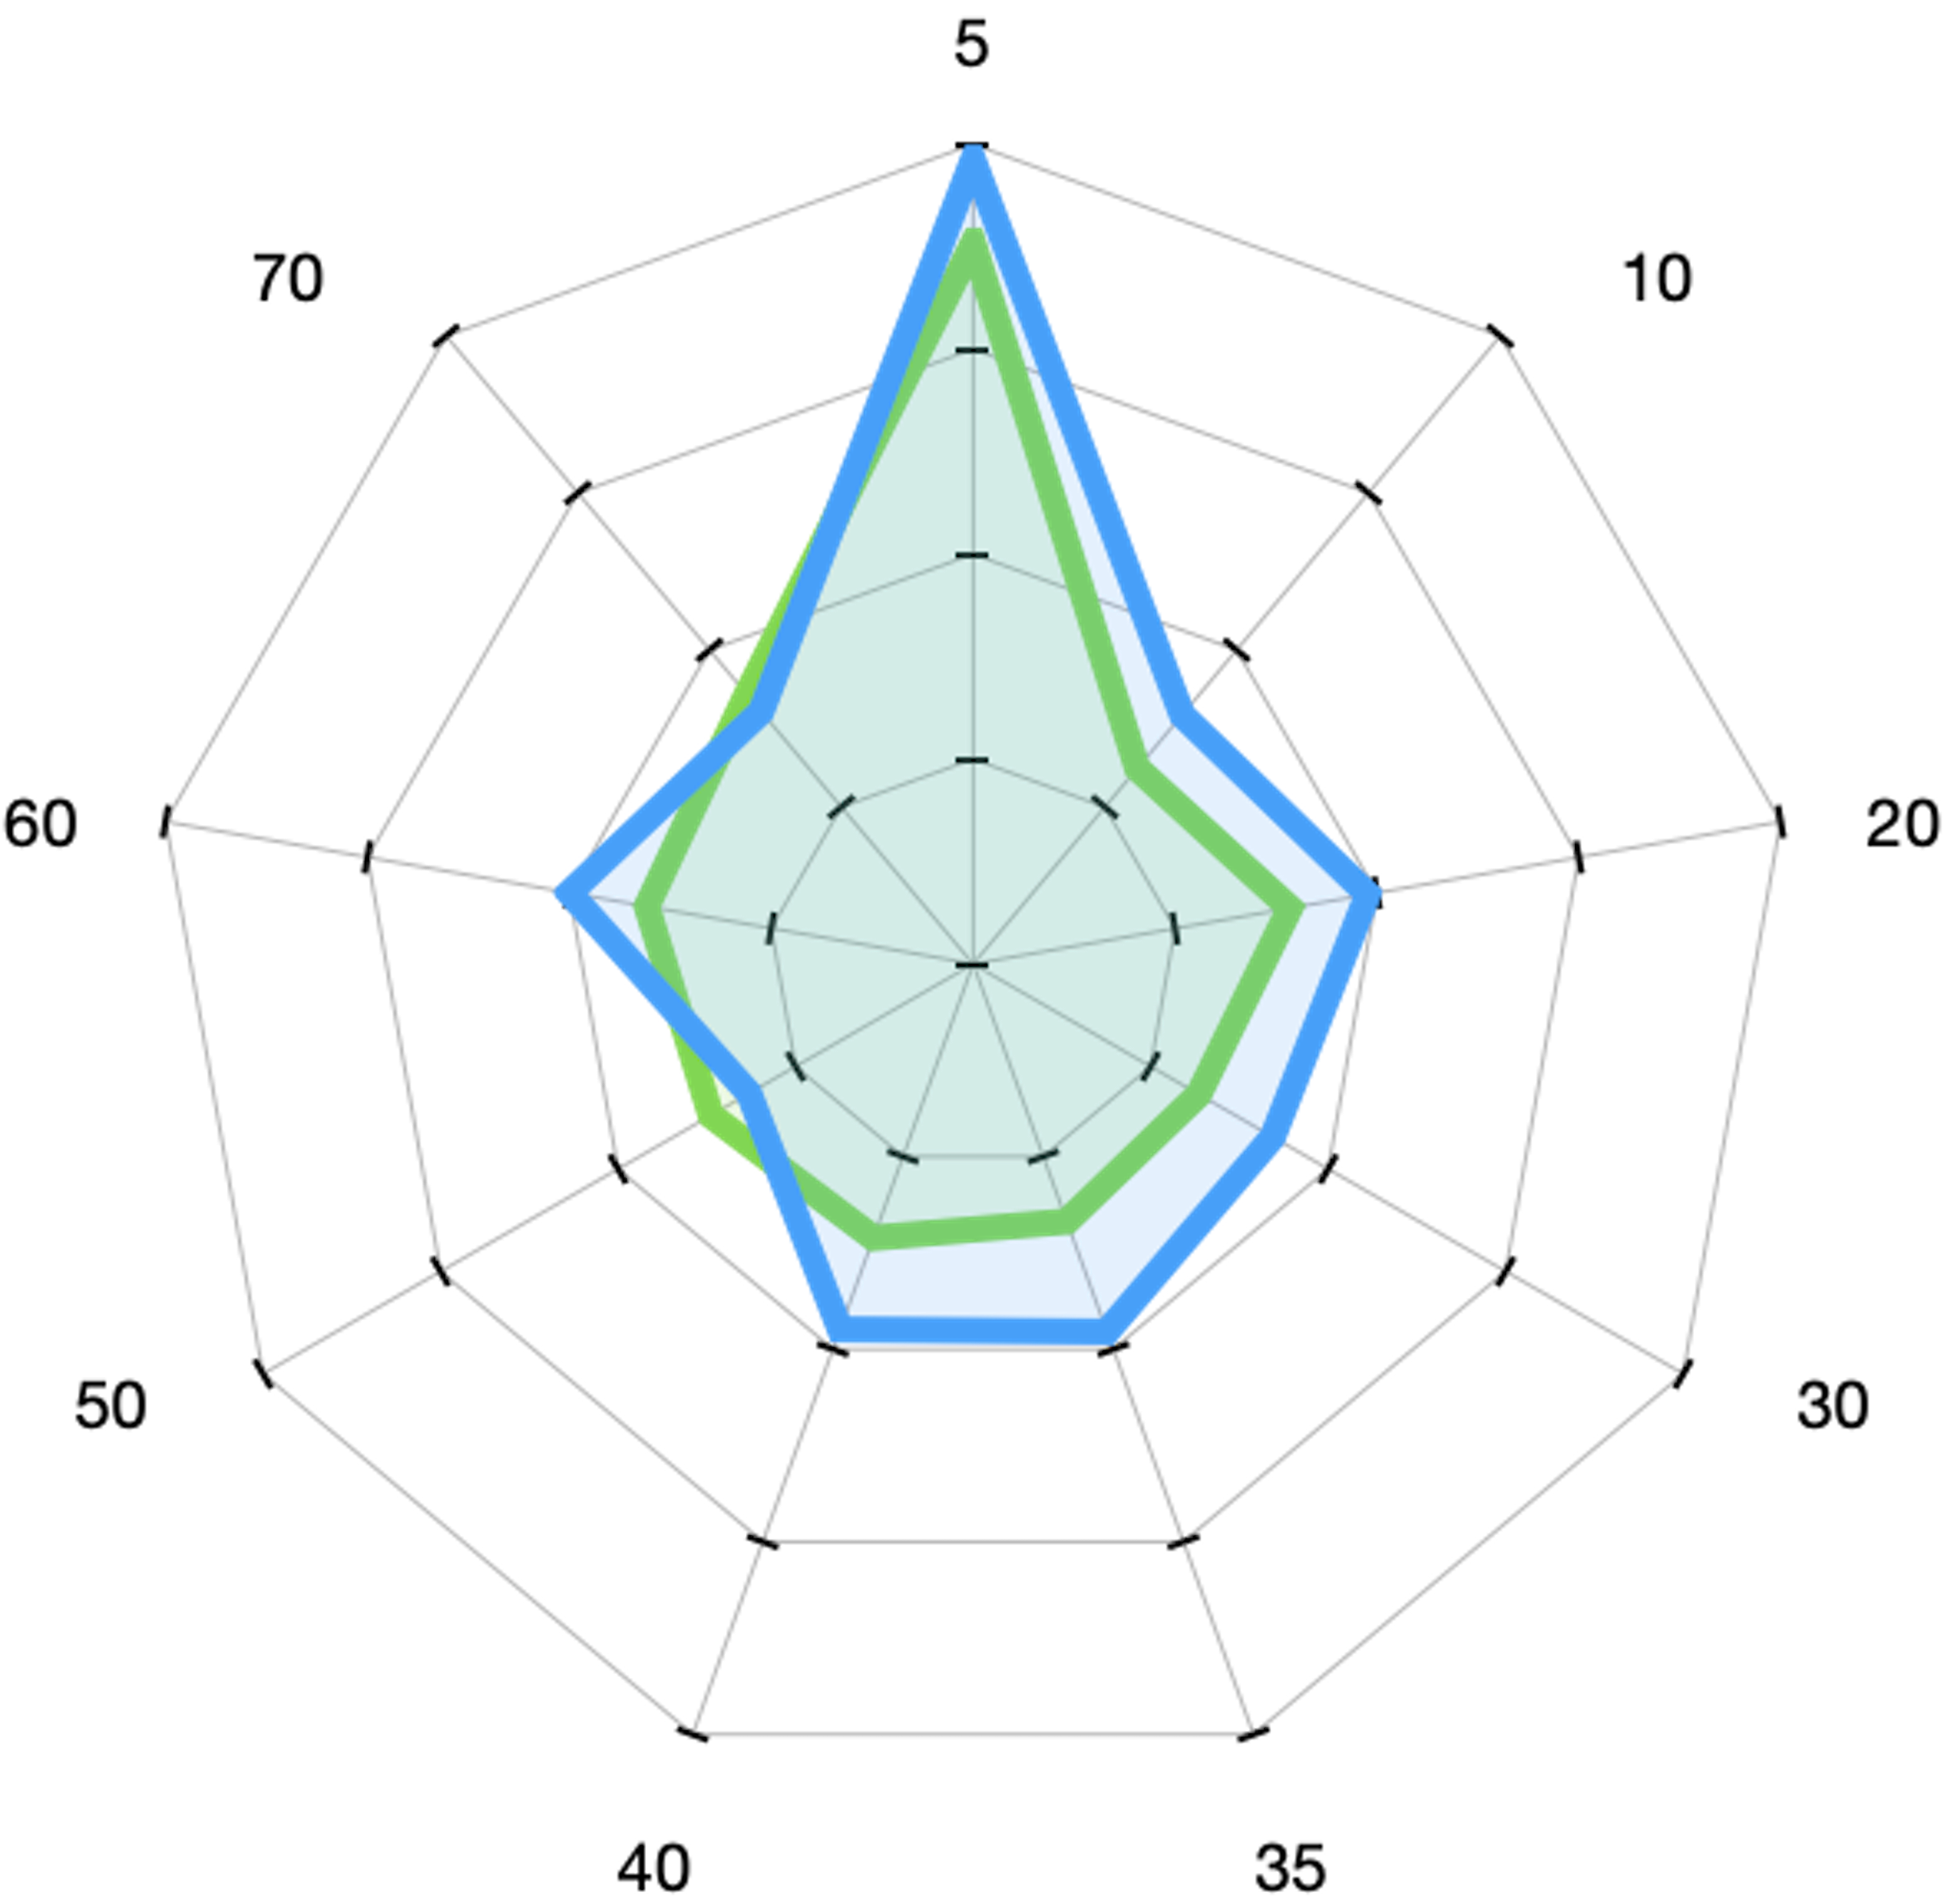
\includegraphics[width=0.4\textwidth, height=0.25\linewidth]{RNN_RMSE_SPIDER.png}\label{fig:RNN_RMSE_SPIDER}}  
\\
\subfloat[BiLSTM Vs Proposed BiLSTM]{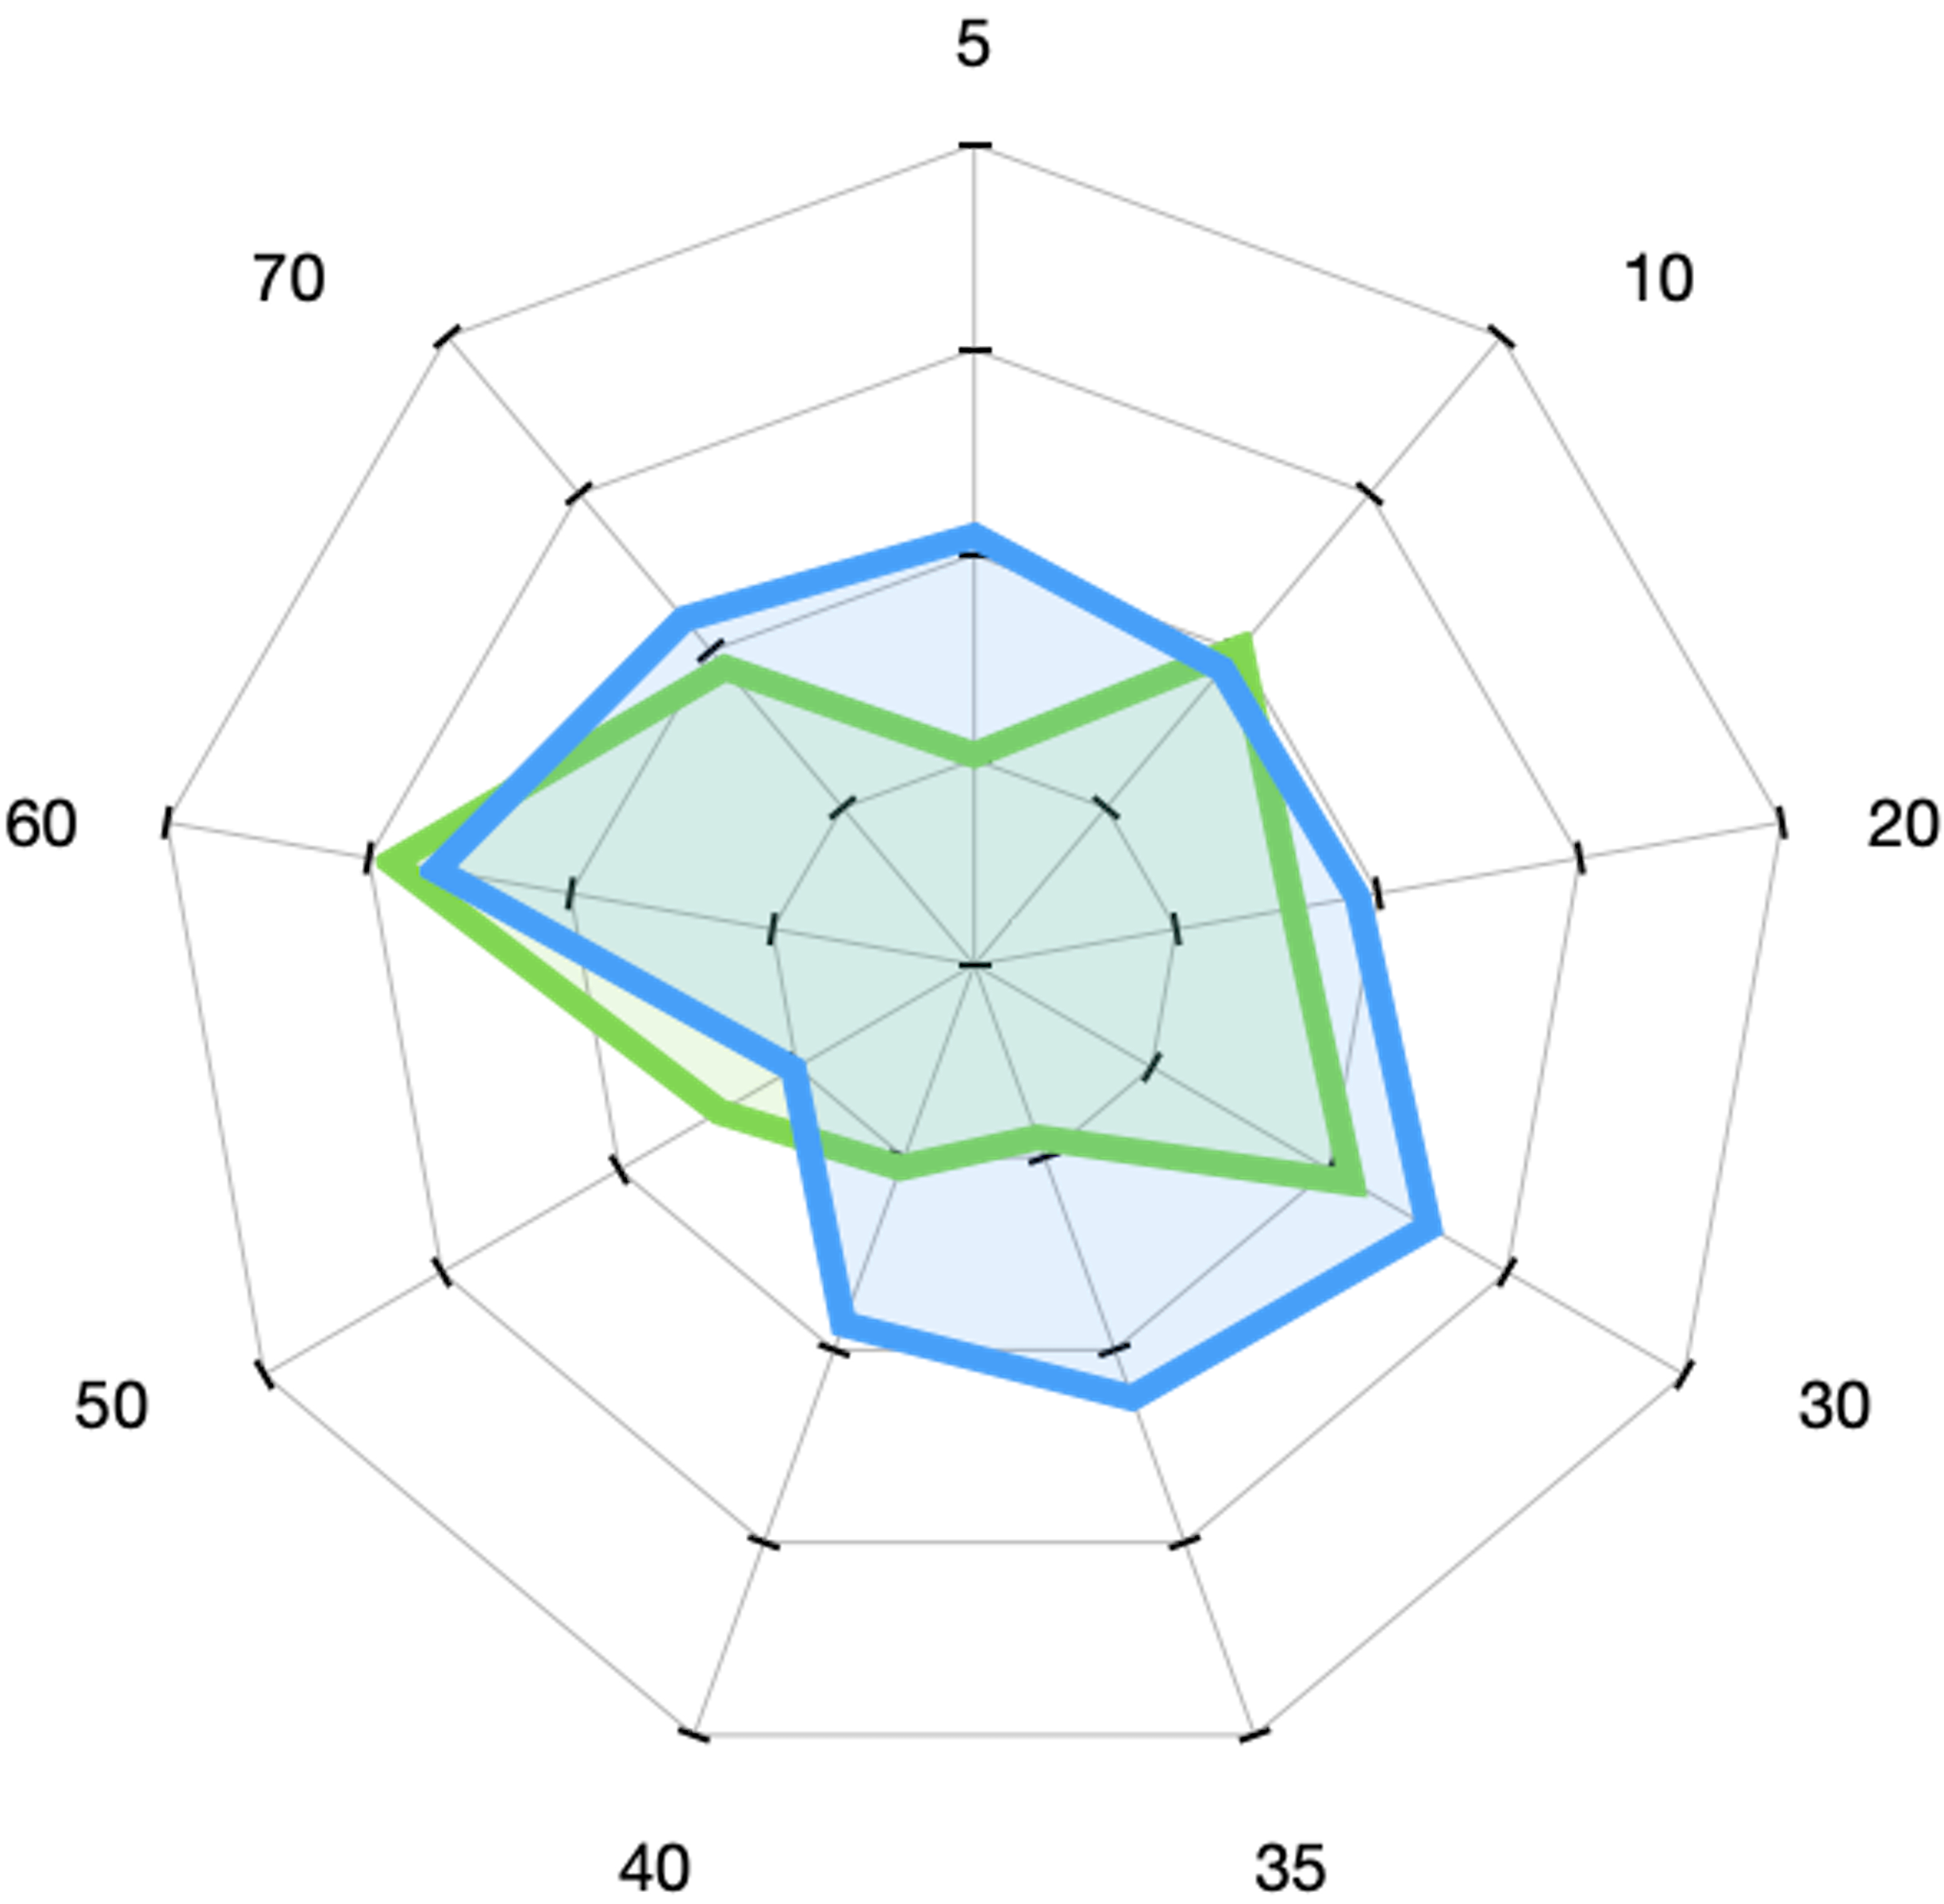
\includegraphics[width=0.4\textwidth, height=0.25\linewidth]{BI-LSTM_RMSE_SPIDER.png}\label{fig:BiLSTM_RMSE_SPIDER}}  
\hfill
\subfloat[GRU Vs Proposed GRU]{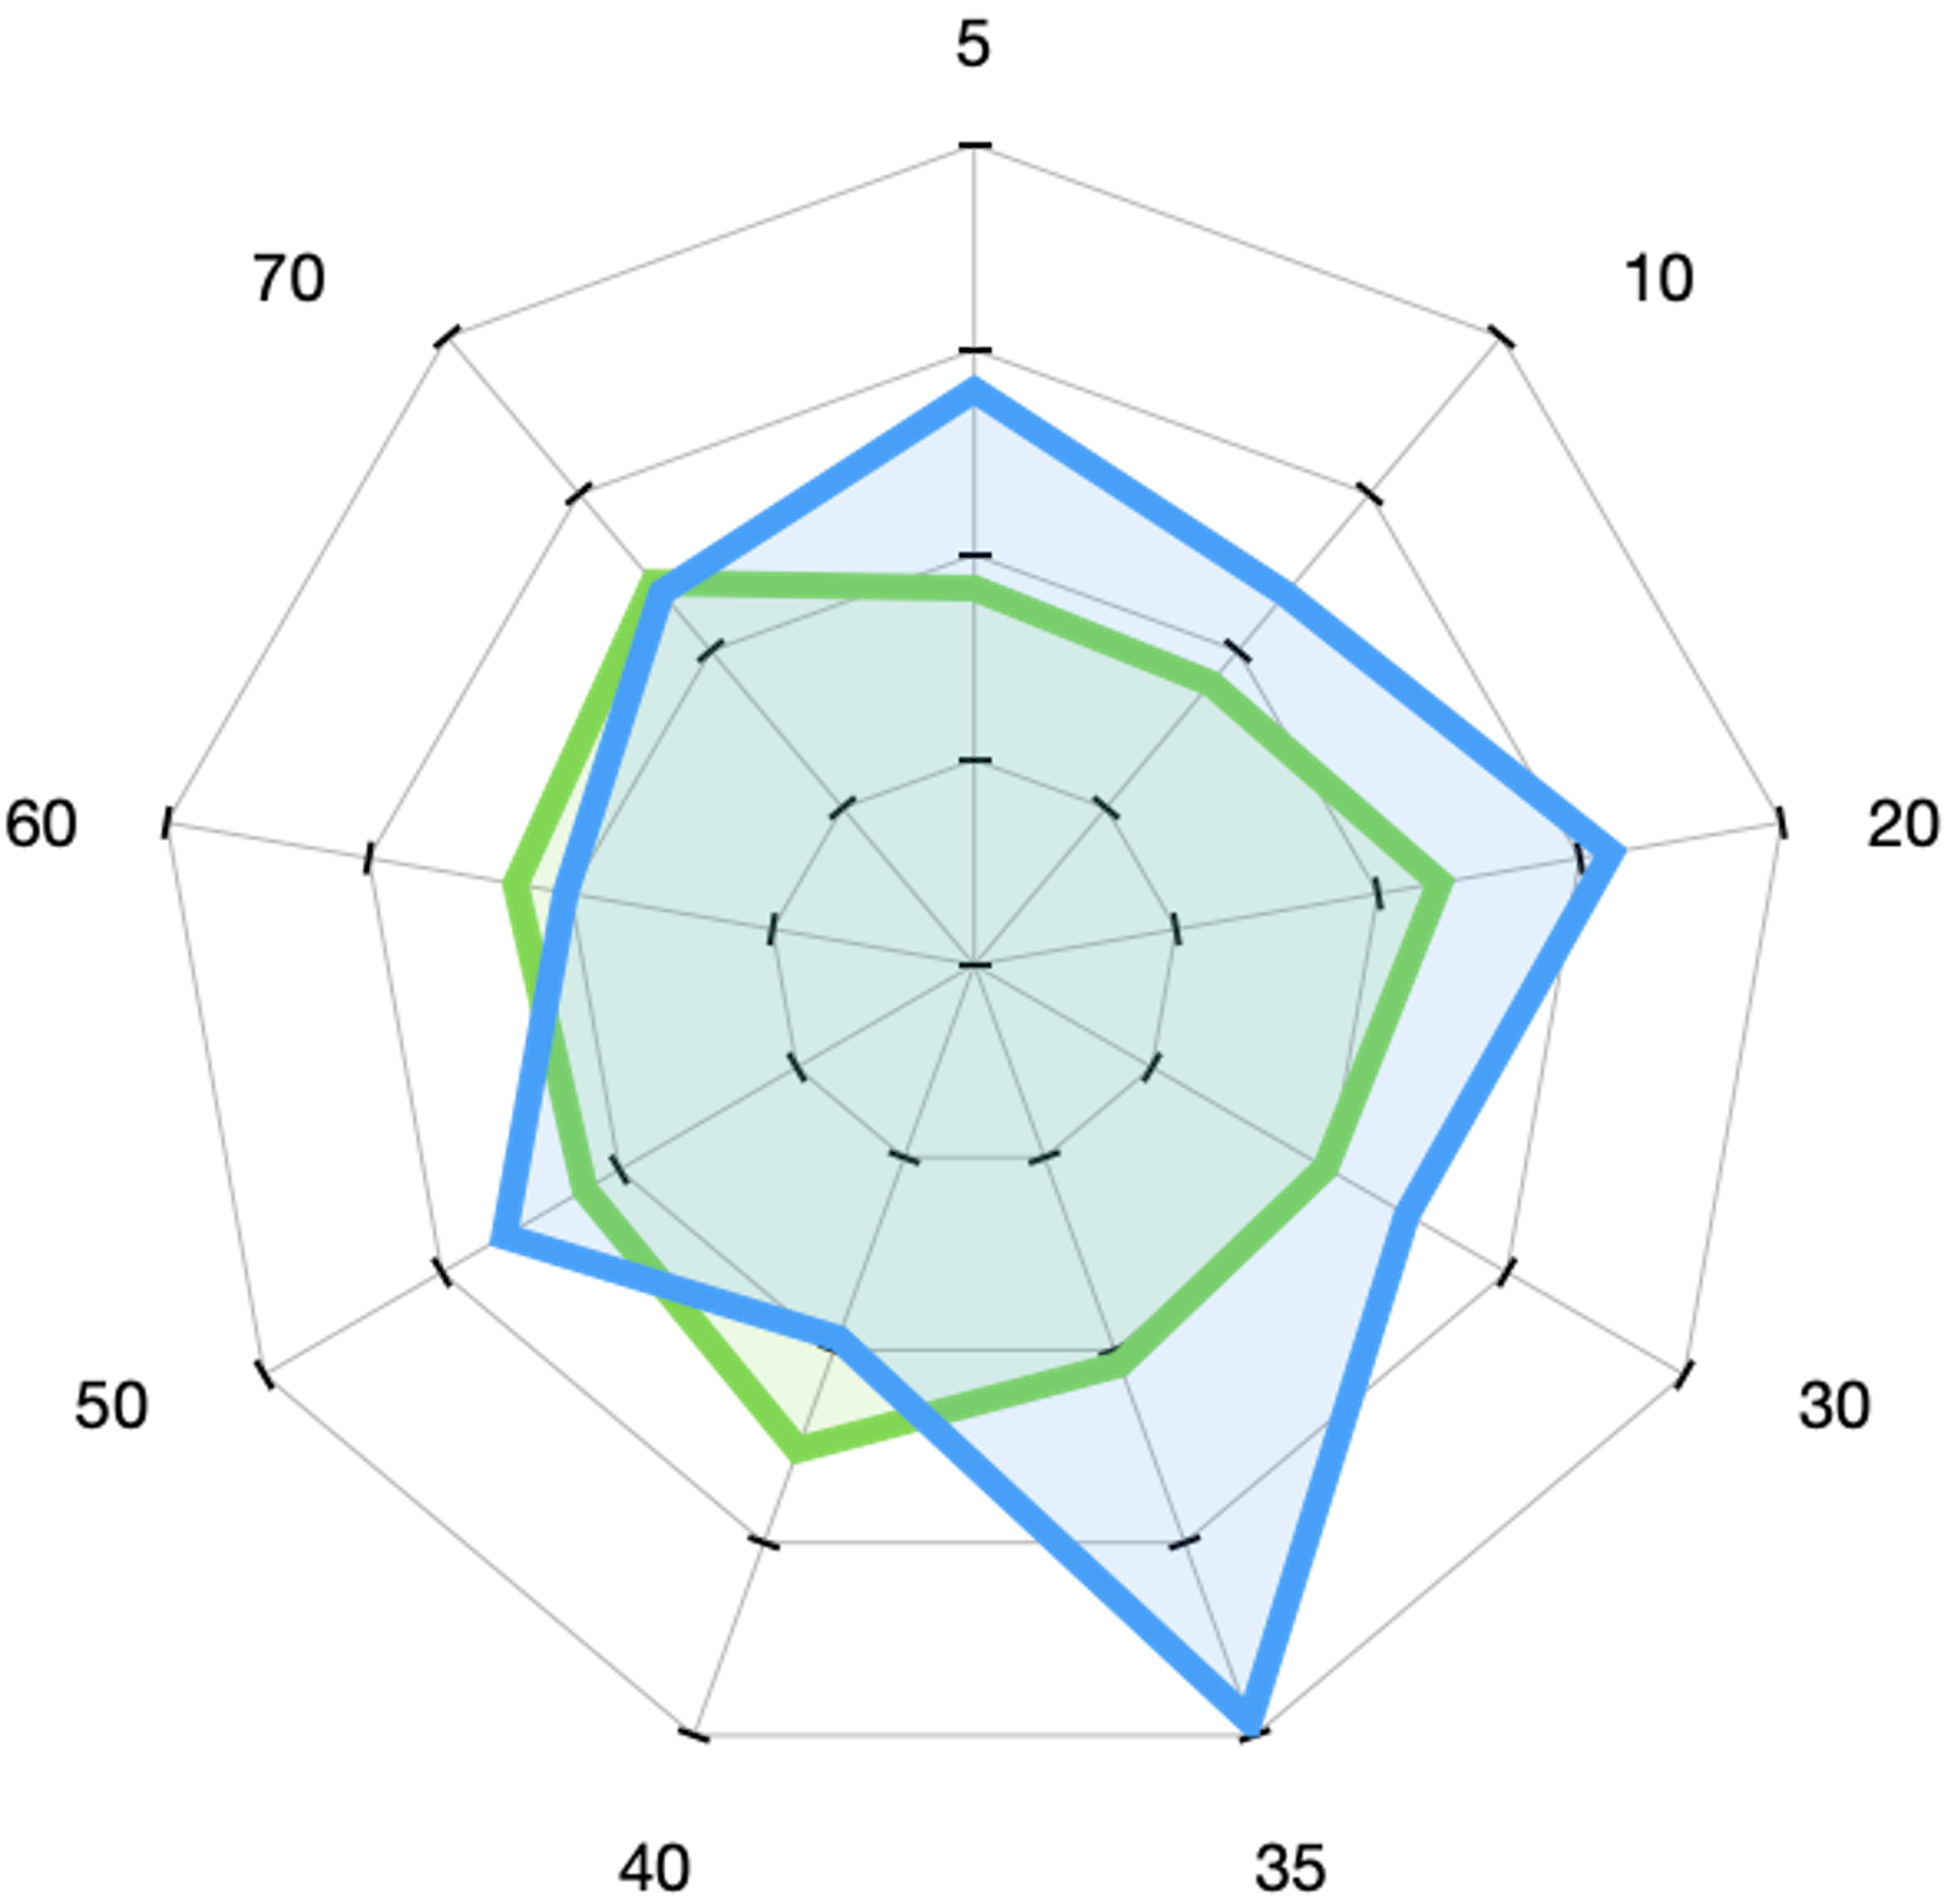
\includegraphics[width=0.4\textwidth, height=0.25\linewidth]{GRU_RMSE_SPIDER.png}\label{fig:GRU_RMSE_SPIDER}}  
  \caption{Comparison of models over RMSE}
  \label{fig:all_models_rmse}
\end{figure} 


\begin{figure}[ht!]
%\centering
\subfloat[LSTM Vs Proposed LSTM]{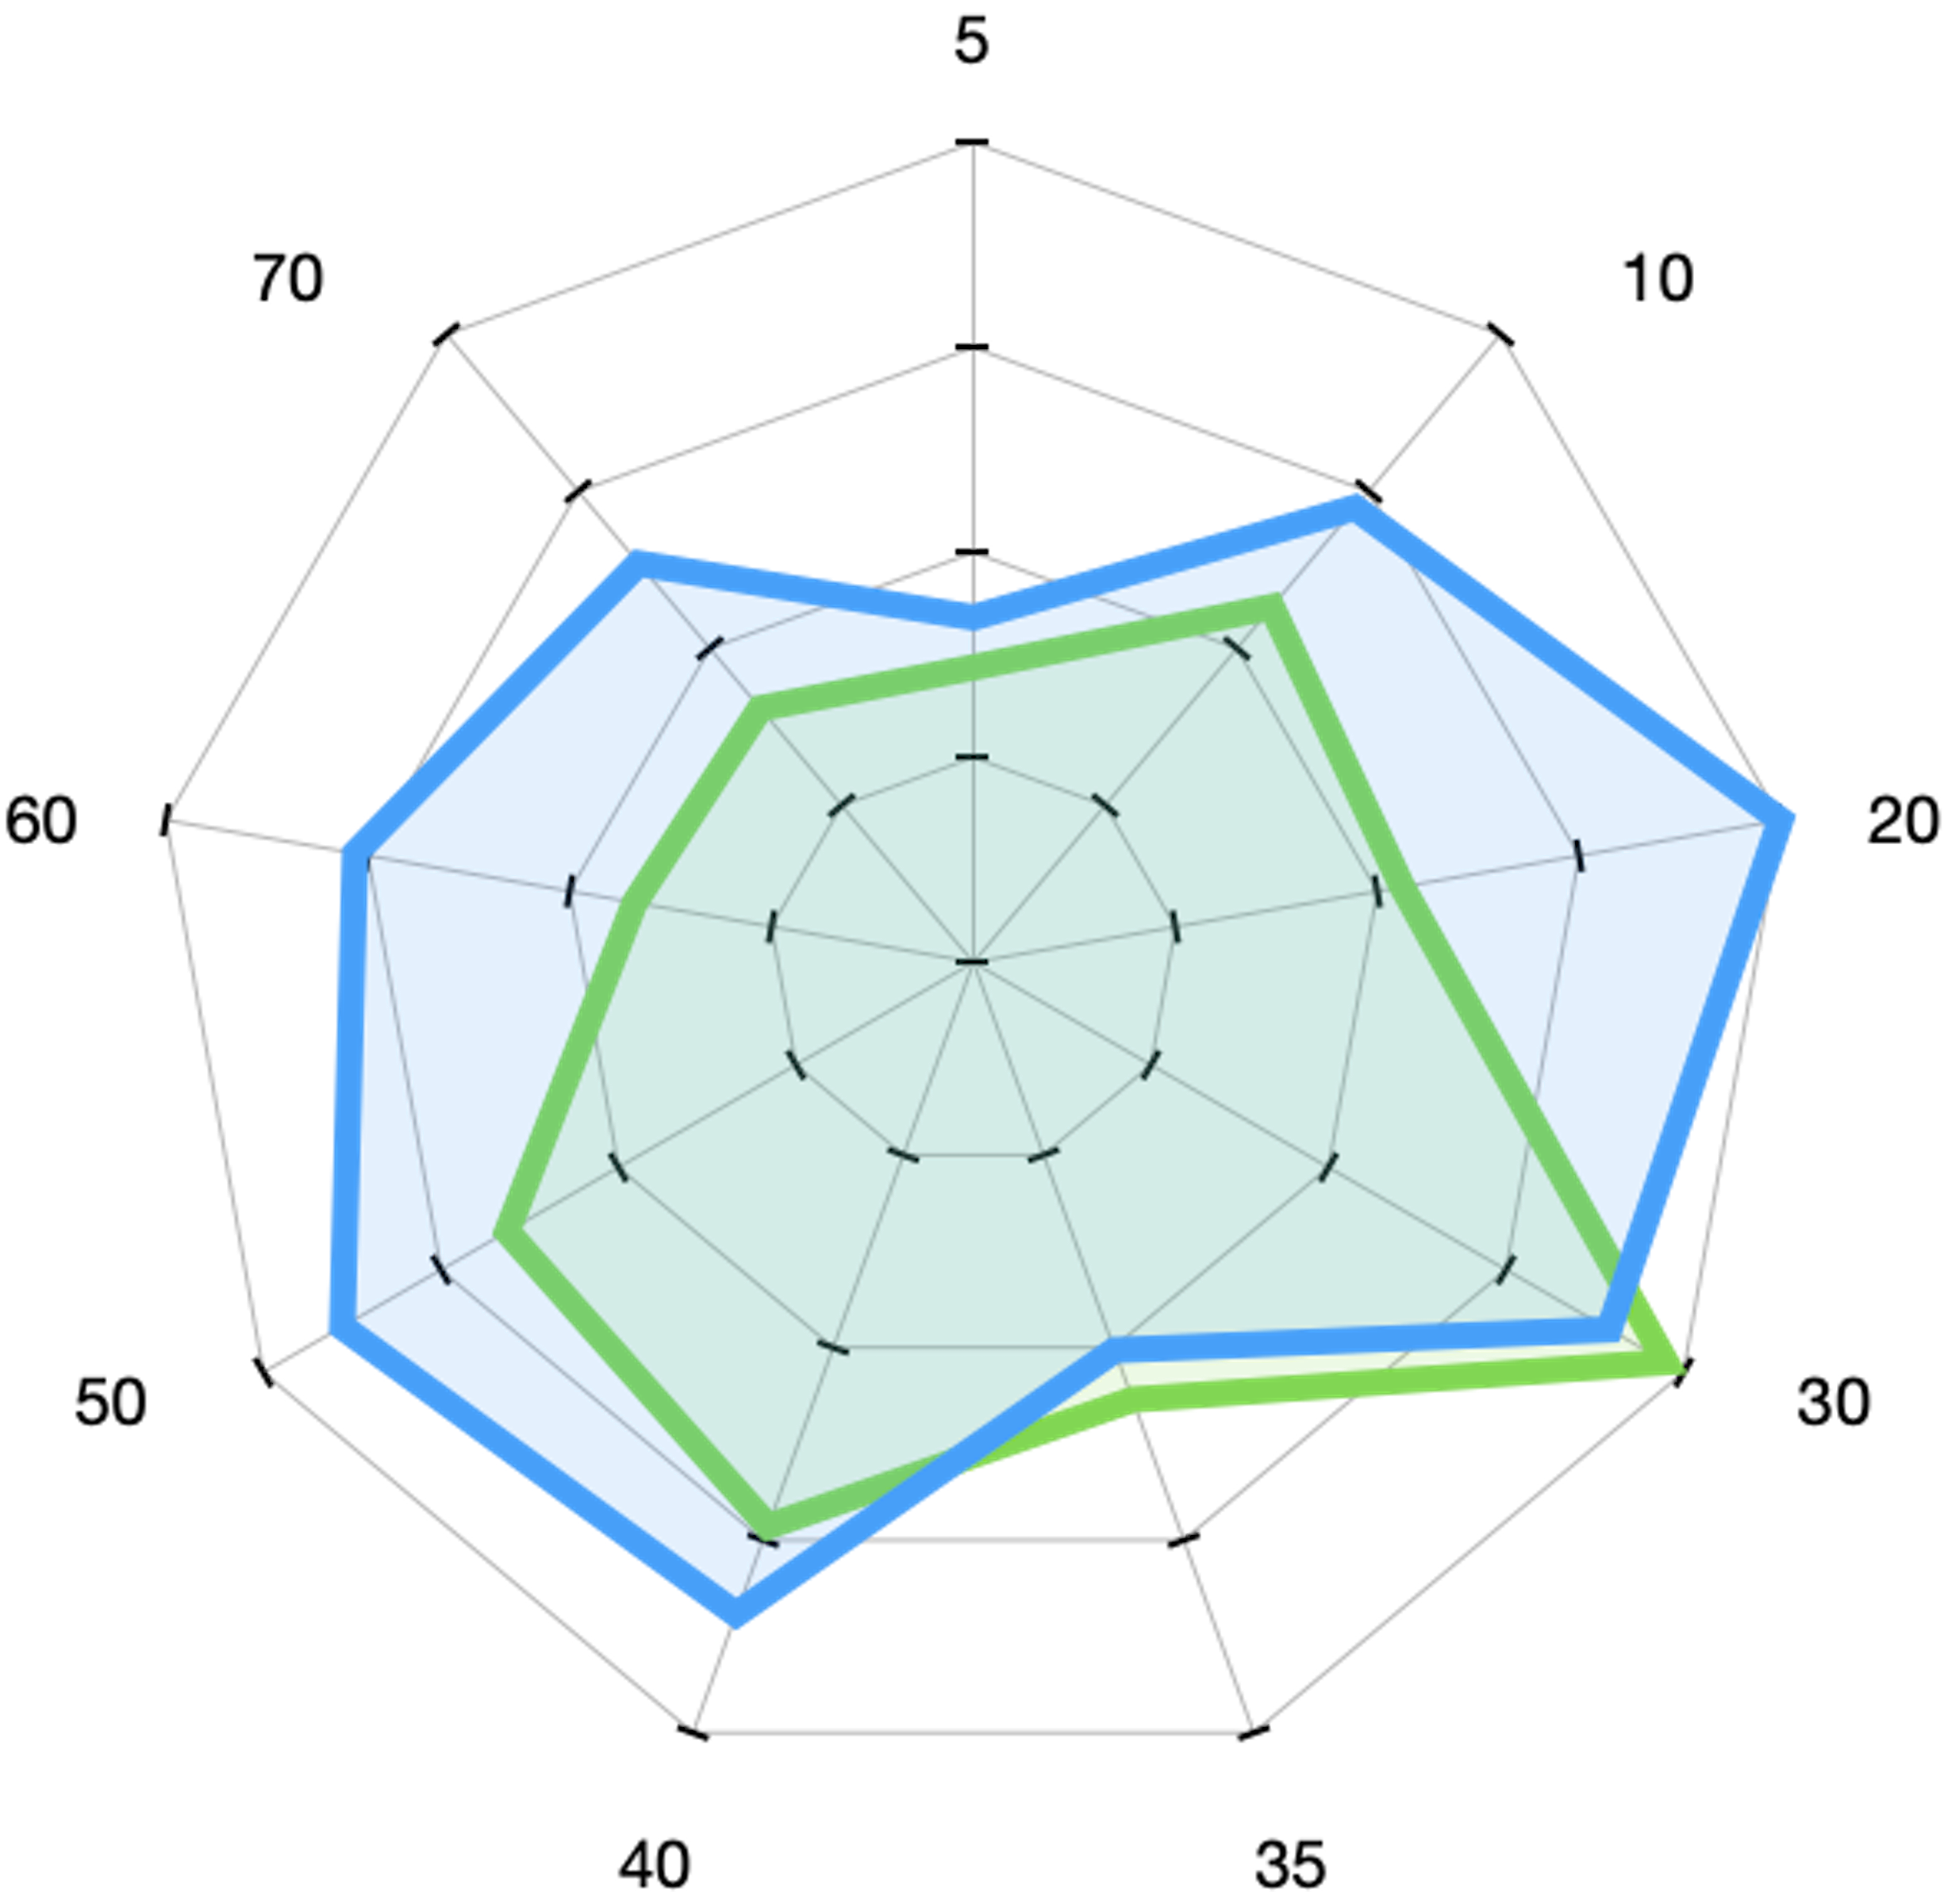
\includegraphics[width=0.4\textwidth, height=0.25\linewidth]{LSTM_RMSE_SPIDER.png}\label{fig:LSTM MAPE SPIDER}}
\hfill
\subfloat[RNN Vs Proposed RNN]{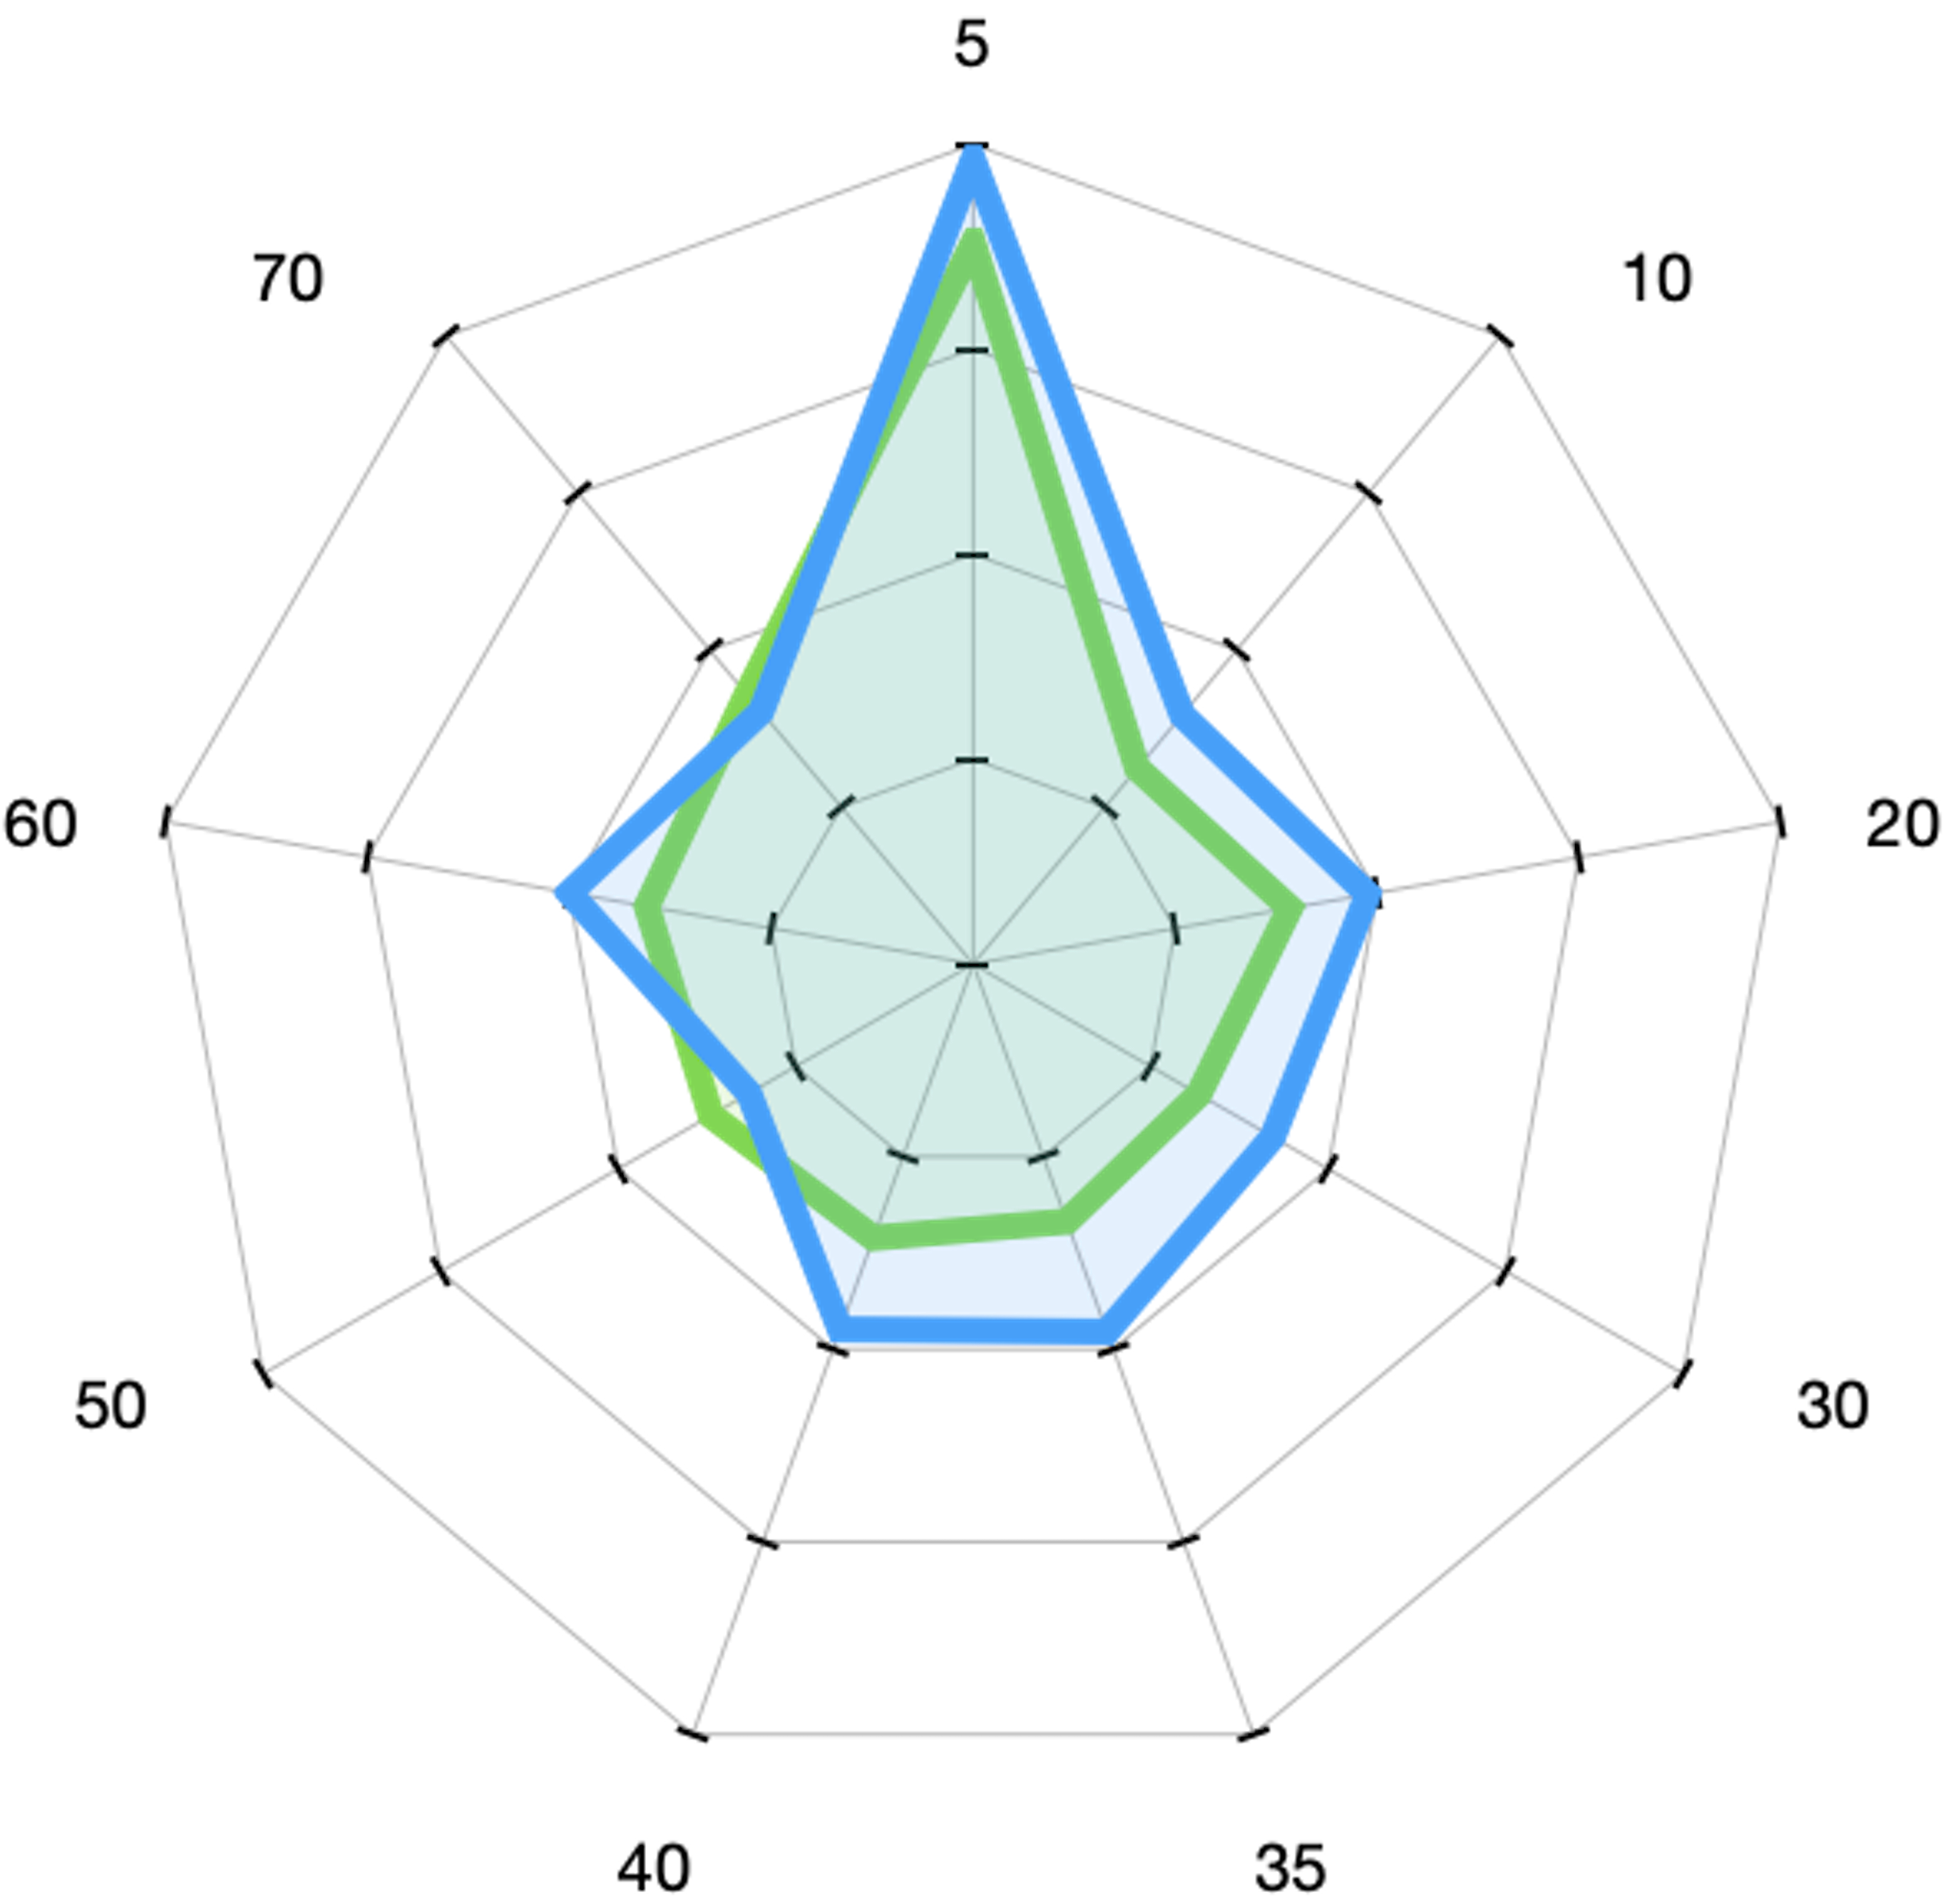
\includegraphics[width=0.4\textwidth, height=0.25\linewidth]{RNN_RMSE_SPIDER.png}\label{fig:RNN_MAPE_SPIDER}}  
\\
\subfloat[BiLSTM Vs Proposed RNN]{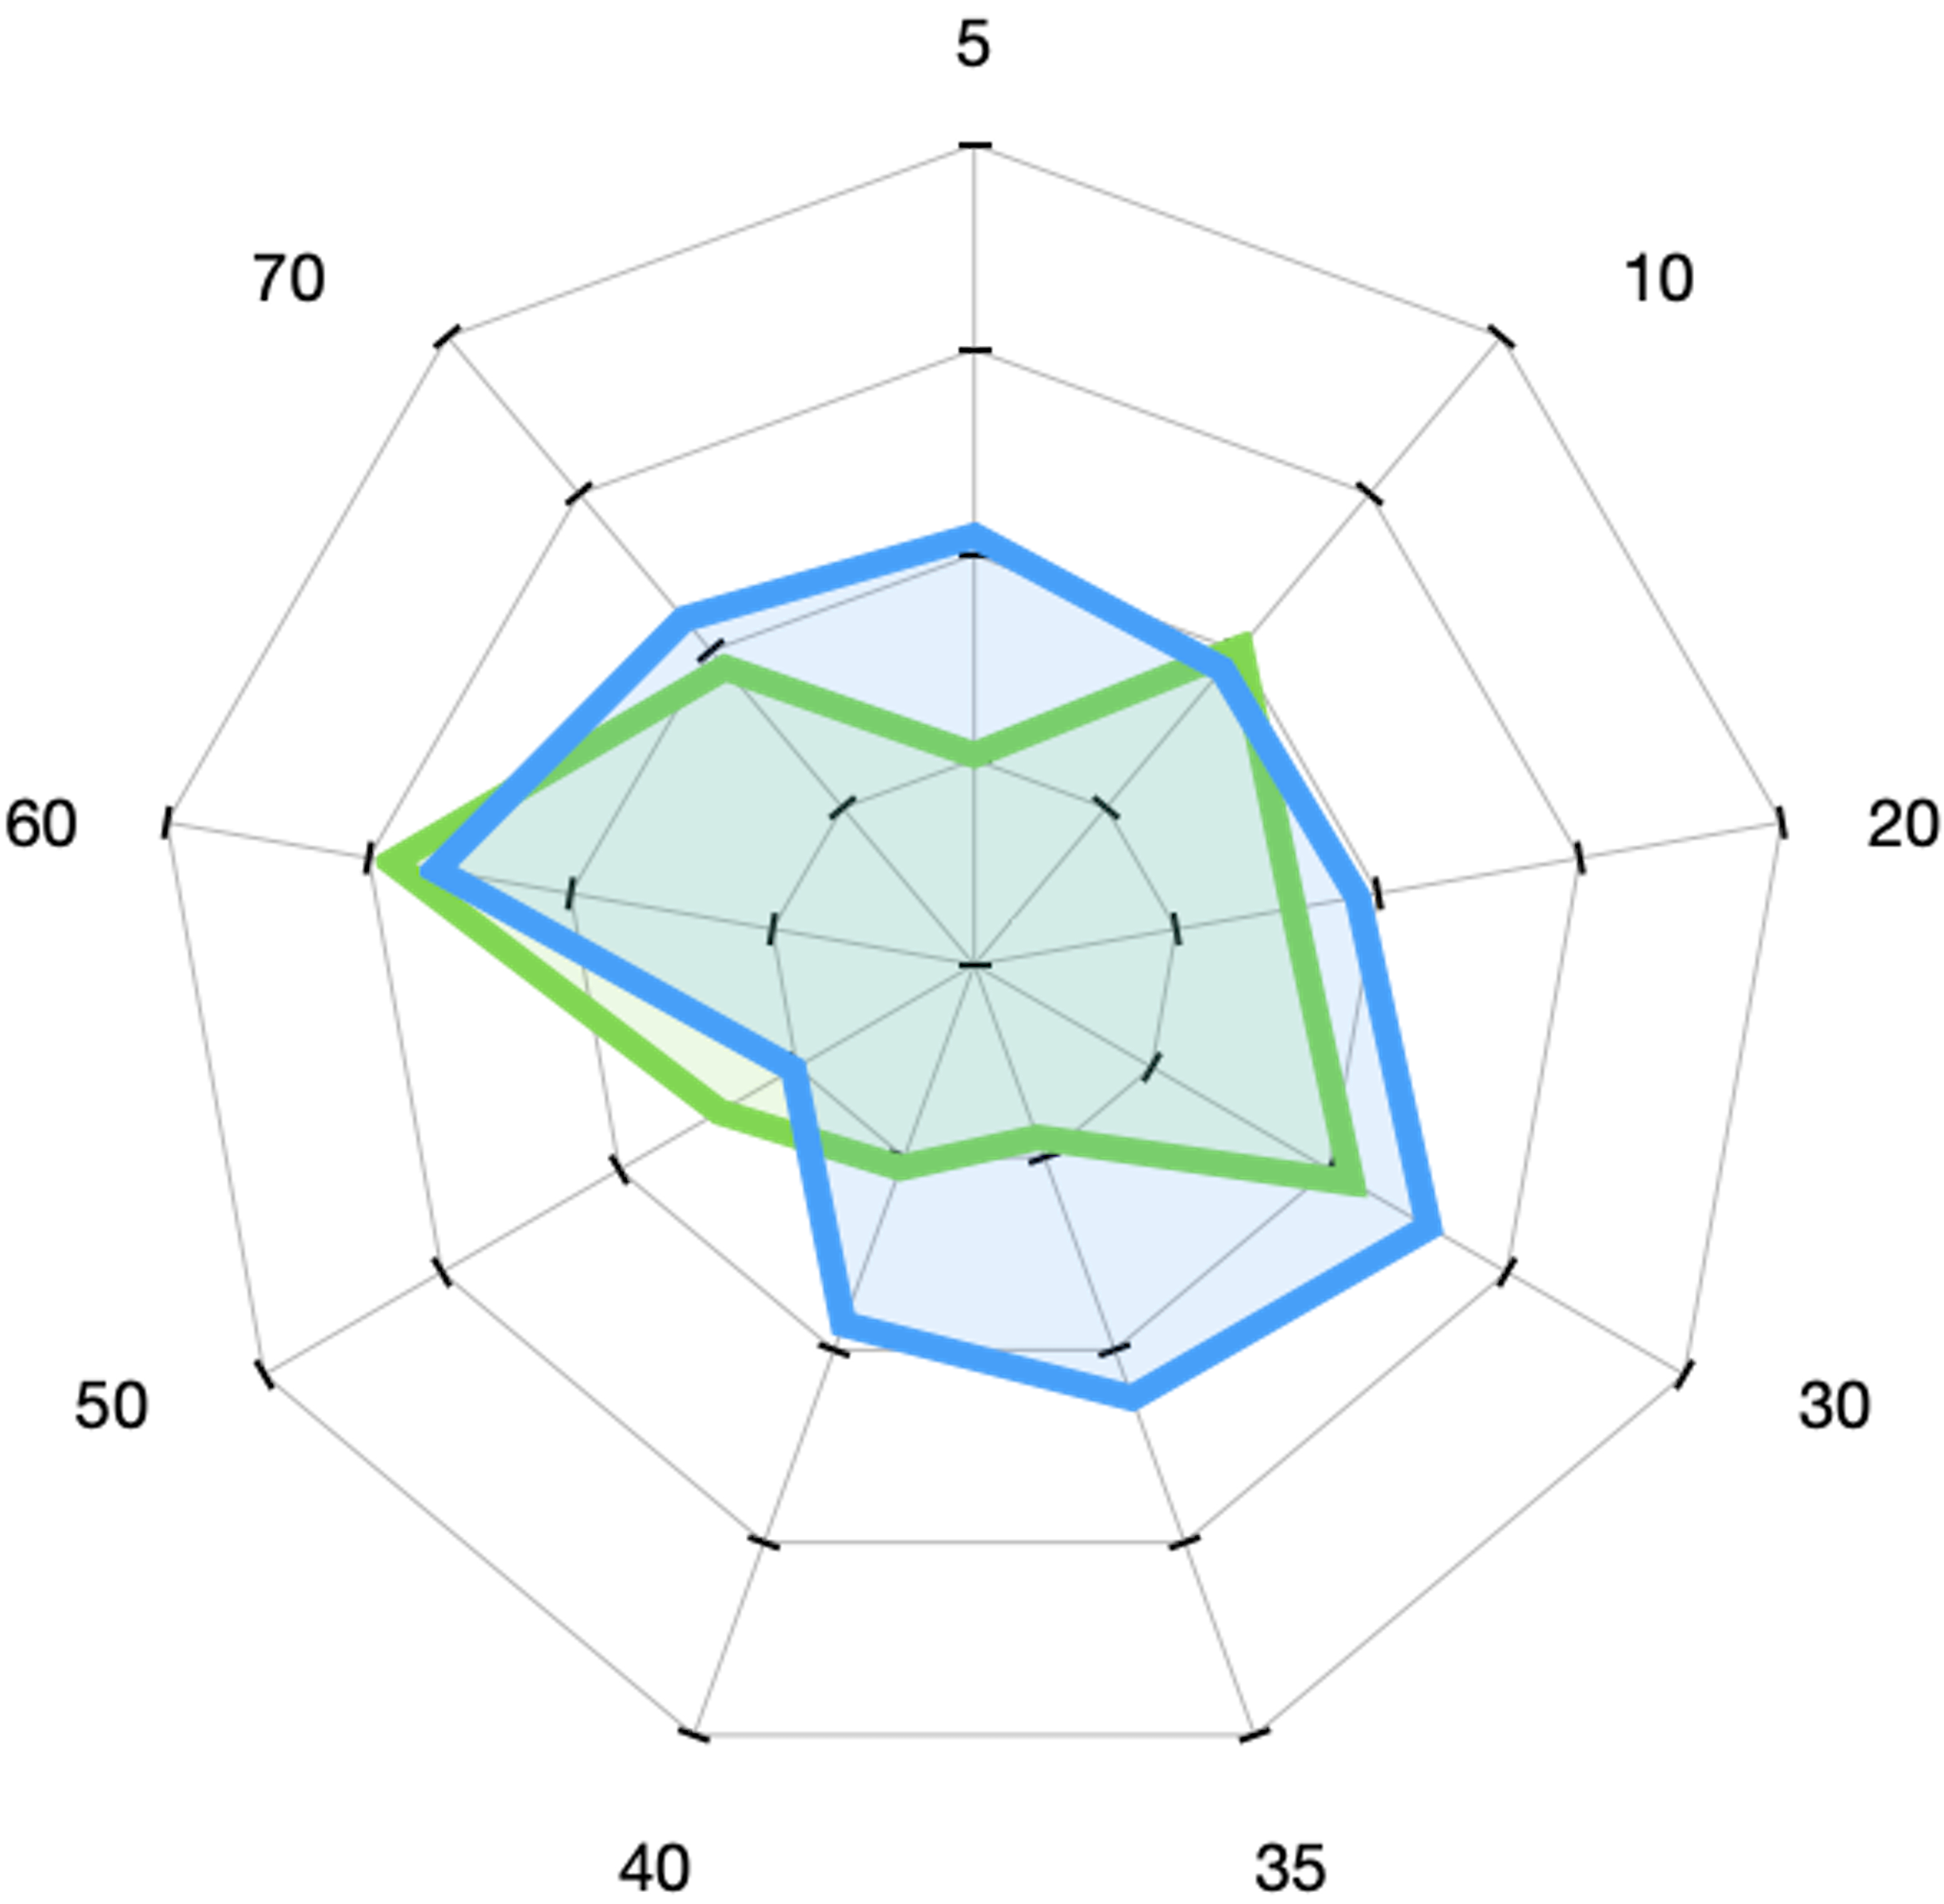
\includegraphics[width=0.4\textwidth, height=0.25\linewidth]{BI-LSTM_RMSE_SPIDER.png}\label{fig:BiLSTM_MAPE_SPIDER}}  
\hfill
\subfloat[GRU Vs Proposed GRU]{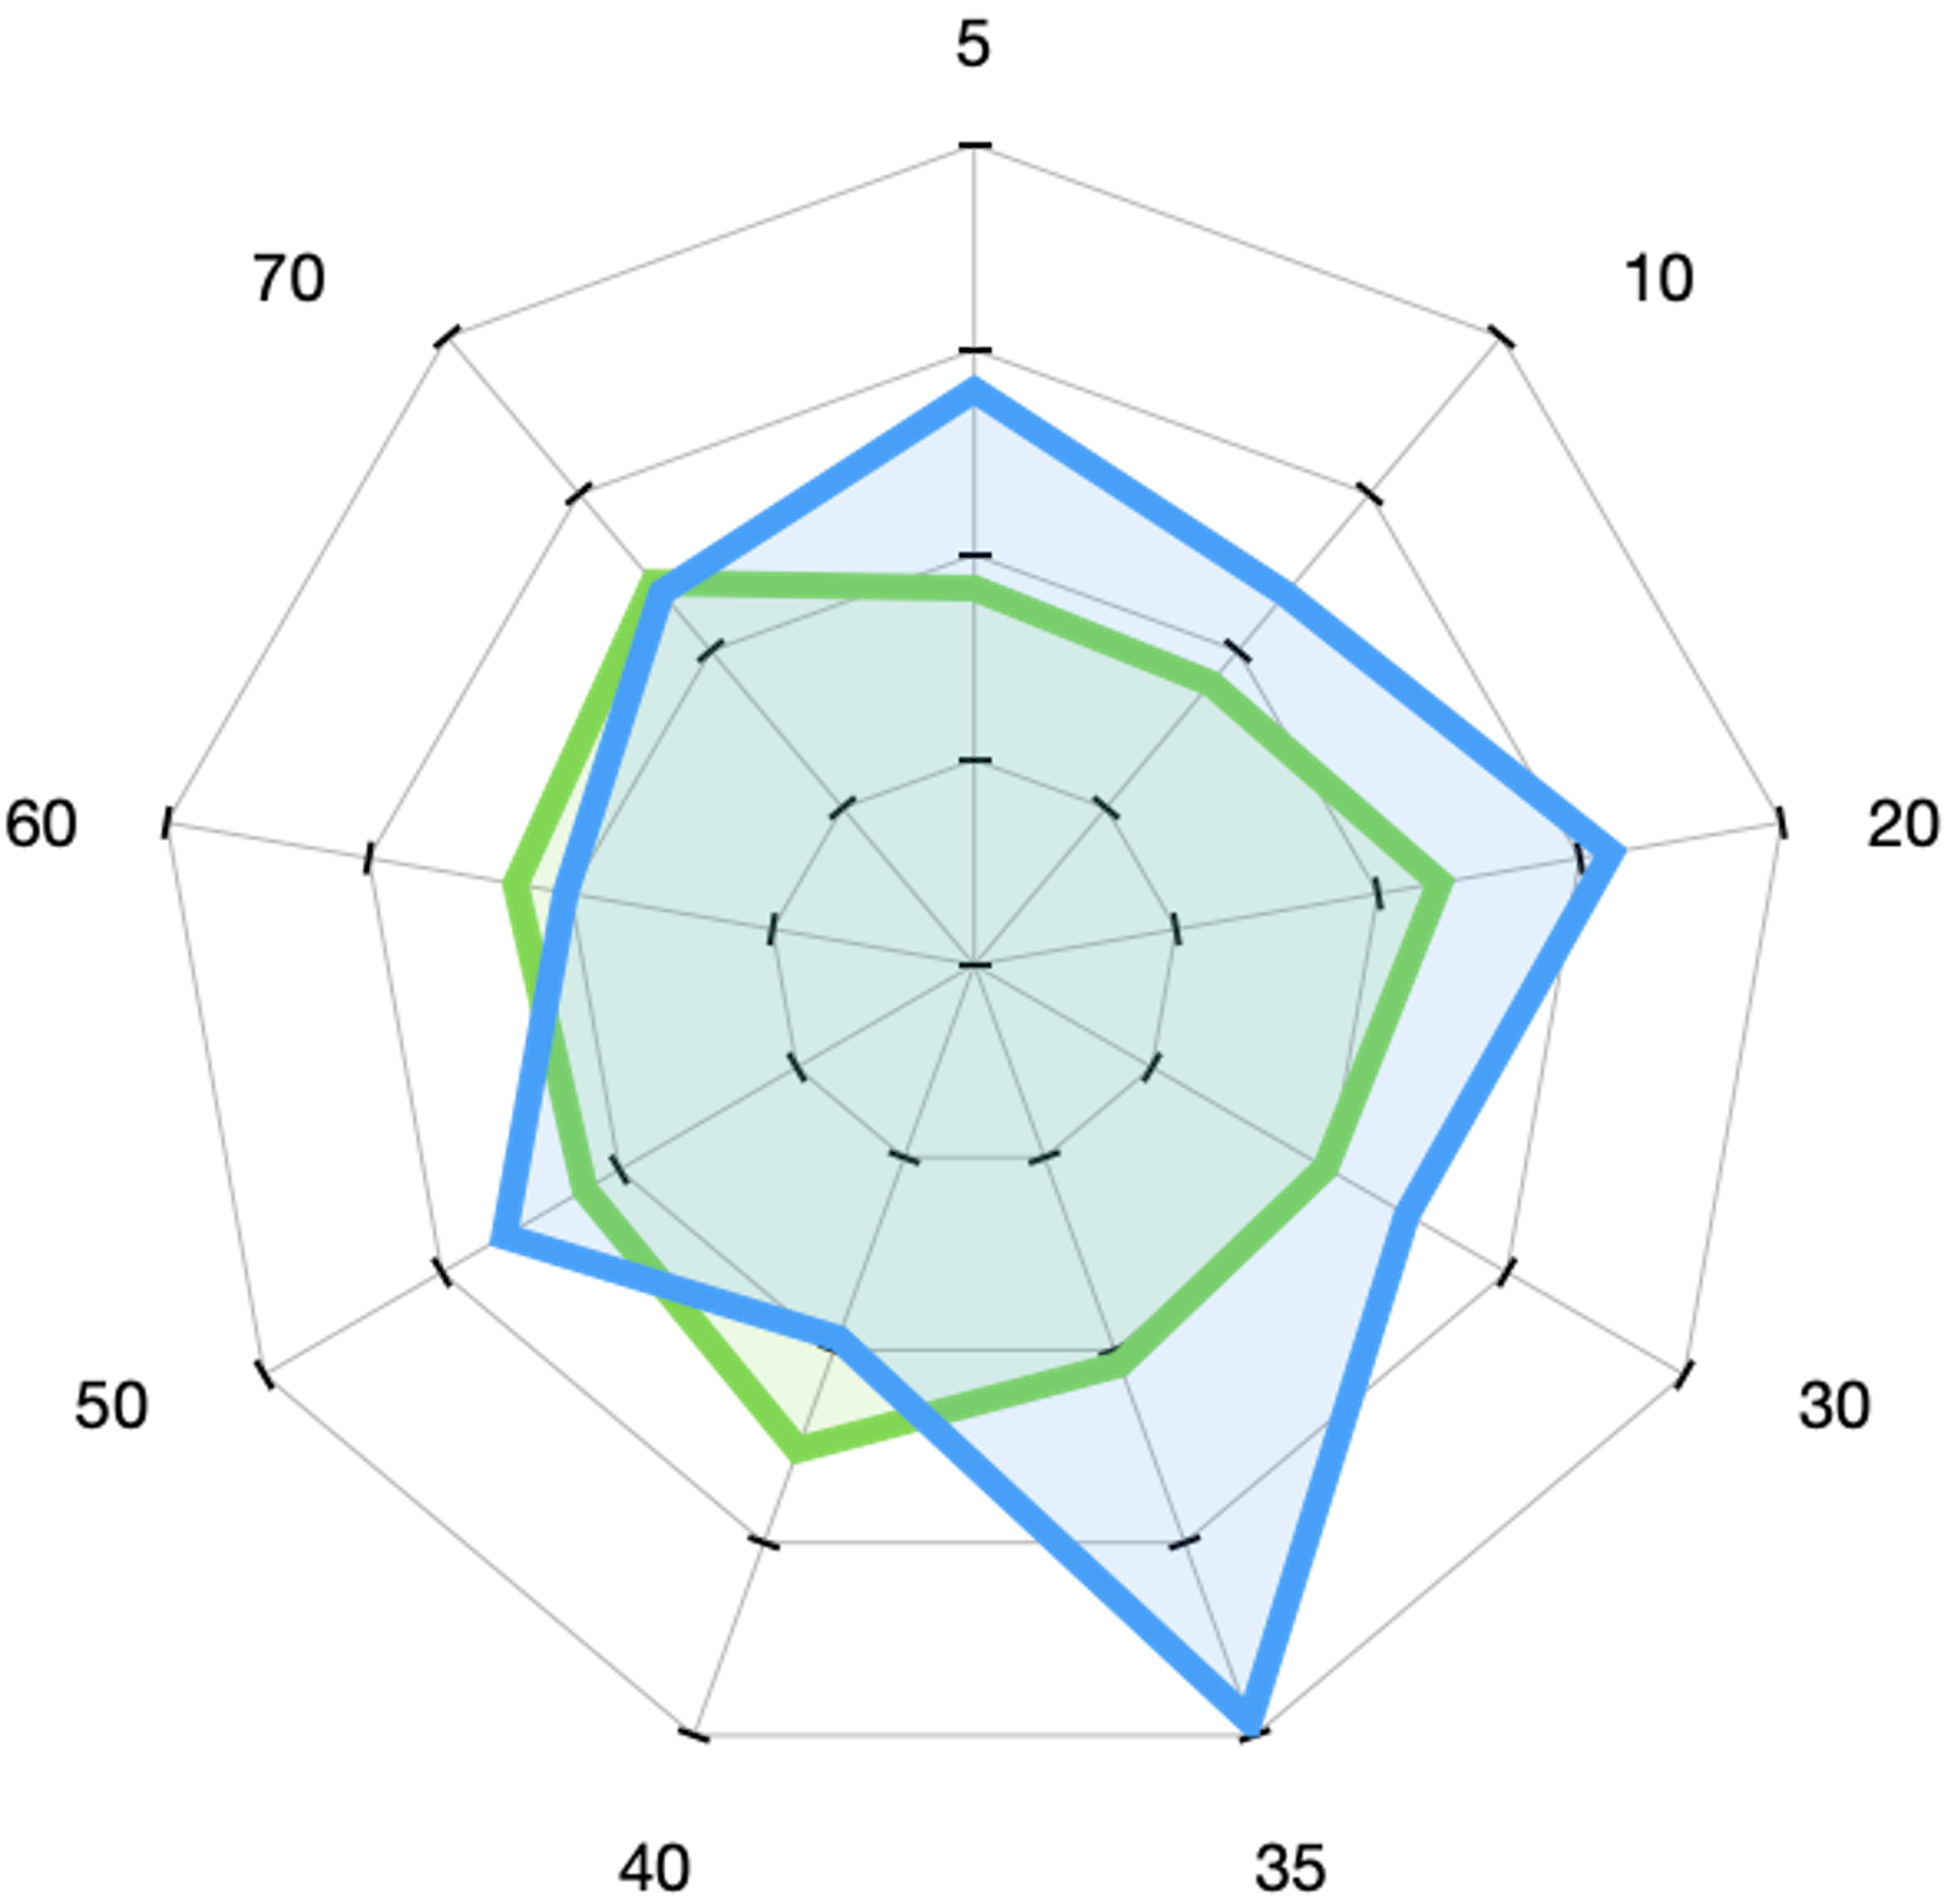
\includegraphics[width=0.4\textwidth, height=0.25\linewidth]{GRU_RMSE_SPIDER.png}\label{fig:GRU_MAPE_SPIDER}}  
  \caption{Comparison of models over MAPE}
  \label{fig:all_models_rmse}
\end{figure} 

\begin{figure}[ht!]
\centering
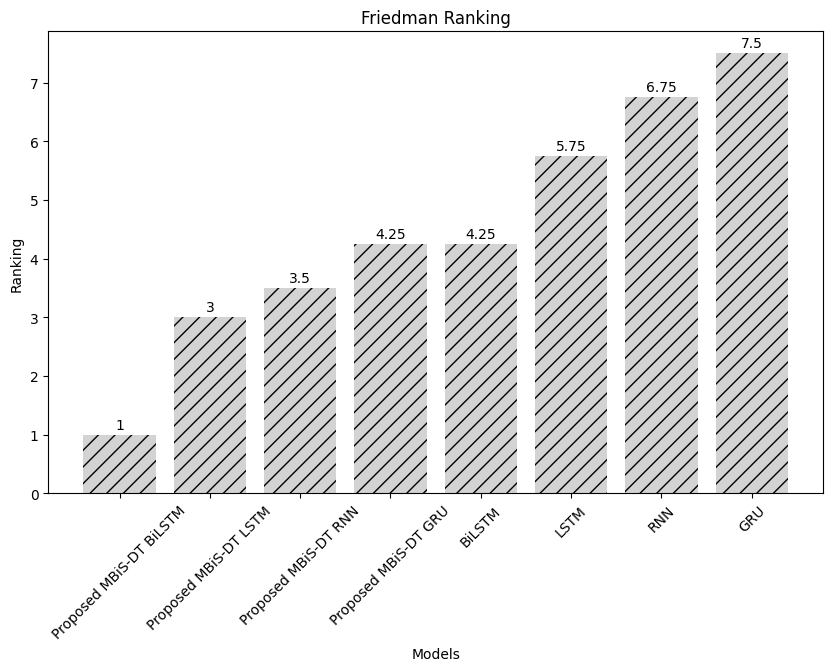
\includegraphics[width=0.9\textwidth, height=0.6\linewidth]{freidman_rank.png}
\label{fig:Friedman}
 \caption{Aggregated Friedman Ranking of proposed (MBiS-DT) models and traditional models over RMSE, MAE, MSE and MAPE.}
 \end{figure} 
%\centering
\pagebreak
Figures \ref{fig:LSTM MAE SPIDER}, \ref{fig:LSTM MAE SPIDER} and \ref{fig:LSTM MAE SPIDER} represents the experiment results for the LSTM where it can be observed that MAE , RMSE and MSE has improved respectively. The improvement in each case is for the eight out of nine experimented shifts which validates the performance of the proposed method. Similarly, Figure \ref{fig:RNN_MAE_SPIDER}, \ref{fig:RNN_RMSE_SPIDER}, \ref{fig:RNN_MSE_SPIDER} depicts the comparative performances for RNN over MAE, RMSE and MSE respectively. The improvement can be observed for most of the cases over all three evaluation metrics. In the similar pattern, Figure \ref{fig:BiLSTM_MAE_SPIDER}, \ref{fig:BiLSTM_RMSE_SPIDER} and \ref{fig:BiLSTM_MSE_SPIDER} represents the comparative view of the proposed method over the BiLSTM model for all experimented measures namely MAE, RMSE and MSE respectively. For every performance metric, improvement can be observed over the traditional approach. The perfor 
 mances comparison over MAE , RMSE and MSE for GRU model is depicted in Figure \ref{fig:GRU_MAE_SPIDER}, \ref{fig:GRU_RMSE_SPIDER} and \ref{fig:GRU_MSE_SPIDER} respectively. These figures also suggest an improvement in the performance of GRU after the implementation of the proposed model.
%\section{This is an example for first level head---section head}\label{sec3}
\begin{table}[ht!]
\begin{tabular}{l|lllll}
\hline
\\
Models& MSE & RMSE & MAE & MAPE & Friedman Ranking\\  
\hline
\\
LSTM            & 7   & 7    & 6   & 3  & 5.75  \\
GRU             & 8   & 8    & 8   & 6  &7.5  \\
BiLSTM          & 4   & 4    & 4   & 5  &4.25  \\
RNN             & 6   & 6    & 7   & 8  &6.75  \\
Proposed LSTM   & 3   & 3    & 2   & 4  & 3  \\
Proposed GRU    & 5   & 5    & 5   & 2   &4.25 \\
Proposed BiLSTM & 1   & 1    & 1   & 1 &1   \\
Proposed RNN    & 2   & 2    & 3   & 7  &3.5  \\ \hline
\end{tabular}
\caption{Ranking of Different Models on the basis of performance measures}
\label{tab:Friedman}
\end{table}
Non Parametric Friedman Ranking of all experimented models is representated in Table \ref{tab:Friedman}

%\begin{table}[!htp]
%\centering
%\begin{tabular}{|c|c|}\hline
%Algorithm&Ranking\\\hline
%LSTM & 5.75\\
%GRU & 7.5\\
%BiLSTM & 4.25\\
%RNN & 6.75\\
%Proposed LSTM & 3\\
%Proposed GRU & 4.25\\
%Proposed BiLSTM & 1\\
%Proposed RNN & 3.5\\
%\hline
%\end{tabular}
%\caption{Average Rankings of the algorithms}
%\label{tab:Friedman}
%\end{table}
Adjusted p-values for $\alpha$=0.05 is represented in Table \ref{tab:pvalue}
%\begin{table}[!htp]
%\centering\scriptsize
%\begin{tabular}{cccc}
%$i$&algorithms&$z=(R_0 - R_i)/SE$&$p$\\
%\hline6&GRU vs. BiLSTM&2.738613&\textbf{0.00617\\
%5&LSTM vs. BiLSTM&1.917029&0.055234\\
%4&BiLSTM vs. RNN&1.917029&0.055234\\
%3&LSTM vs. GRU&0.821584&0.411314\\
%2&GRU vs. RNN&0.821584&0.411314\\
%1&LSTM vs. RNN&0&1\\
%\hline
%\end{tabular}
%\caption{P-values Table for $\alpha=0.05$}
%\label{tab:pvalue}
%\end{table}

\begin{table}[!htbp]
\centering\scriptsize
\begin{tabular}{cccc}
\hline
$i$&algorithms&$z=(R_0 - R_i)/SE$&$p$\\
\hline28&GRU vs. Proposed BiLSTM&3.752777&\textbf{0.000175}\\
27&RNN vs. Proposed BiLSTM&3.319764&\textbf{0.000901}\\
26&LSTM vs. Proposed BiLSTM&2.742414&\textbf{0.006099}\\
25&GRU vs. Proposed LSTM&2.598076&\textbf{0.009375}\\
24&GRU vs. Proposed RNN&2.309401&\textbf{0.020921}\\
23&RNN vs. Proposed LSTM&2.165064&\textbf{0.030383}\\
22&GRU vs. BiLSTM&1.876388&0.060602\\
21&GRU vs. Proposed GRU&1.876388&0.060602\\
20&BiLSTM vs. Proposed BiLSTM&1.876388&0.060602\\
19&RNN vs. Proposed RNN&1.876388&0.060602\\
18&Proposed GRU vs. Proposed BiLSTM&1.876388&0.060602\\
17&LSTM vs. Proposed LSTM&1.587713&0.112351\\
16&BiLSTM vs. RNN&1.443376&0.148915\\
15&RNN vs. Proposed GRU&1.443376&0.148915\\
14&Proposed BiLSTM vs. Proposed RNN&1.443376&0.148915\\
13&LSTM vs. Proposed RNN&1.299038&0.193931\\
12&Proposed LSTM vs. Proposed BiLSTM&1.154701&0.248213\\
11&LSTM vs. GRU&1.010363&0.312321\\
10&LSTM vs. BiLSTM&0.866025&0.386476\\
9&LSTM vs. Proposed GRU&0.866025&0.386476\\
8&BiLSTM vs. Proposed LSTM&0.721688&0.470486\\
7&Proposed LSTM vs. Proposed GRU&0.721688&0.470486\\
6&LSTM vs. RNN&0.57735&0.563703\\
5&GRU vs. RNN&0.433013&0.665006\\
4&BiLSTM vs. Proposed RNN&0.433013&0.665006\\
3&Proposed GRU vs. Proposed RNN&0.433013&0.665006\\
2&Proposed LSTM vs. Proposed RNN&0.288675&0.77283\\
1&BiLSTM vs. Proposed GRU&0&1\\
\hline
\end{tabular}
\caption{P-values Table for $\alpha=0.05$}
\label{tab:pvalue}
\end{table}
\pagebreak

\section{Conclusion}
In this study, a deep learning approach has been utilized to forecast the temperature.In this research endeavor, the potential of deep learning in enhancing temperature prediction has been explored. The intricate interplay between temperature and deep learning techniques has been illuminated, offering insights into the accuracy and efficacy of data-driven prediction models.

Through an in-depth investigation into time-series satellite data and the utilization of deep learning methodologies, our study has underscored the capacity of neural networks to capture complex temporal dependencies within temperature patterns. This capacity extends to short and mid-term predictions, where the predictive performance showcases the power of data-driven insights.

Our research journey encompassed the intricate modeling of temperature fluctuations, Exploring the details of how things change over time in an easy-to-understand way. By supporting the strengths of deep learning architectures, we have pushed the boundaries of predictive accuracy, contributing to a broader understanding of climate variations and their implications.

%\section*{Declarations}

%Some journals require declarations to be submitted in a standardised format. Please check the Instructions for Authors of the journal to which you are submitting to see if you need to complete this section. If yes, your manuscript must contain the following sections under the heading `Declarations':

%\begin{itemize}
%\item Funding
%\item Conflict of interest/Competing interests (check journal-specific guidelines for which heading to use)
%\item Ethics approval 
%\item Consent to participate
%\item Consent for publication
%\item Availability of data and materials
%\item Code availability 
%\item Authors' contributions
%\end{itemize}

%\noindent
%If any of the sections are not relevant to your manuscript, please include the heading and write `Not applicable' for that section. 

%%===================================================%%
%% For presentation purpose, we have included        %%
%% \bigskip command. please ignore this.             %%
%%===================================================%%
%\bigskip
%\begin{flushleft}%
%Editorial Policies for:

%\bigskip\noindent
%Springer journals and proceedings: \url{https://www.springer.com/gp/editorial-policies}

%\bigskip\noindent
%Nature Portfolio journals: \url{https://www.nature.com/nature-research/editorial-policies}

%\bigskip\noindent
%\textit{Scientific Reports}: \url{https://www.nature.com/srep/journal-policies/editorial-policies}

%\bigskip\noindent
%BMC journals: %\url{https://www.biomedcentral.com/getpublished/editorial-policies}
%\end{flushleft}

%\begin{appendices}

%\section{Section title of first appendix}\label{secA1}

%An appendix contains supplementary information that is not an essential part of the text itself but which may be helpful in providing a more comprehensive understanding of the research problem or it is information that is too cumbersome to be included in the body of the paper.
%\end{appendices}
\bibliography{sn-bibliography}% common bib file
%% if required, the content of .bbl file can be included here once bbl is generated
%%\input sn-article.bbl


\end{document}
